%%%%%%%%%%%%%%%%%%%%%%%%%%%%%%%%%%%%%%%%%%%%%%%%%%%%%%%%%%%%%%%%%%%%%%%%
\clearpage
\section{Sheared and deformed objects}
\label{sec:ShearedAndDeformed}

\subsection{Non-equilibrium static form factor of a reptating chain}
~\\

\begin{figure}[htb]
\begin{center}
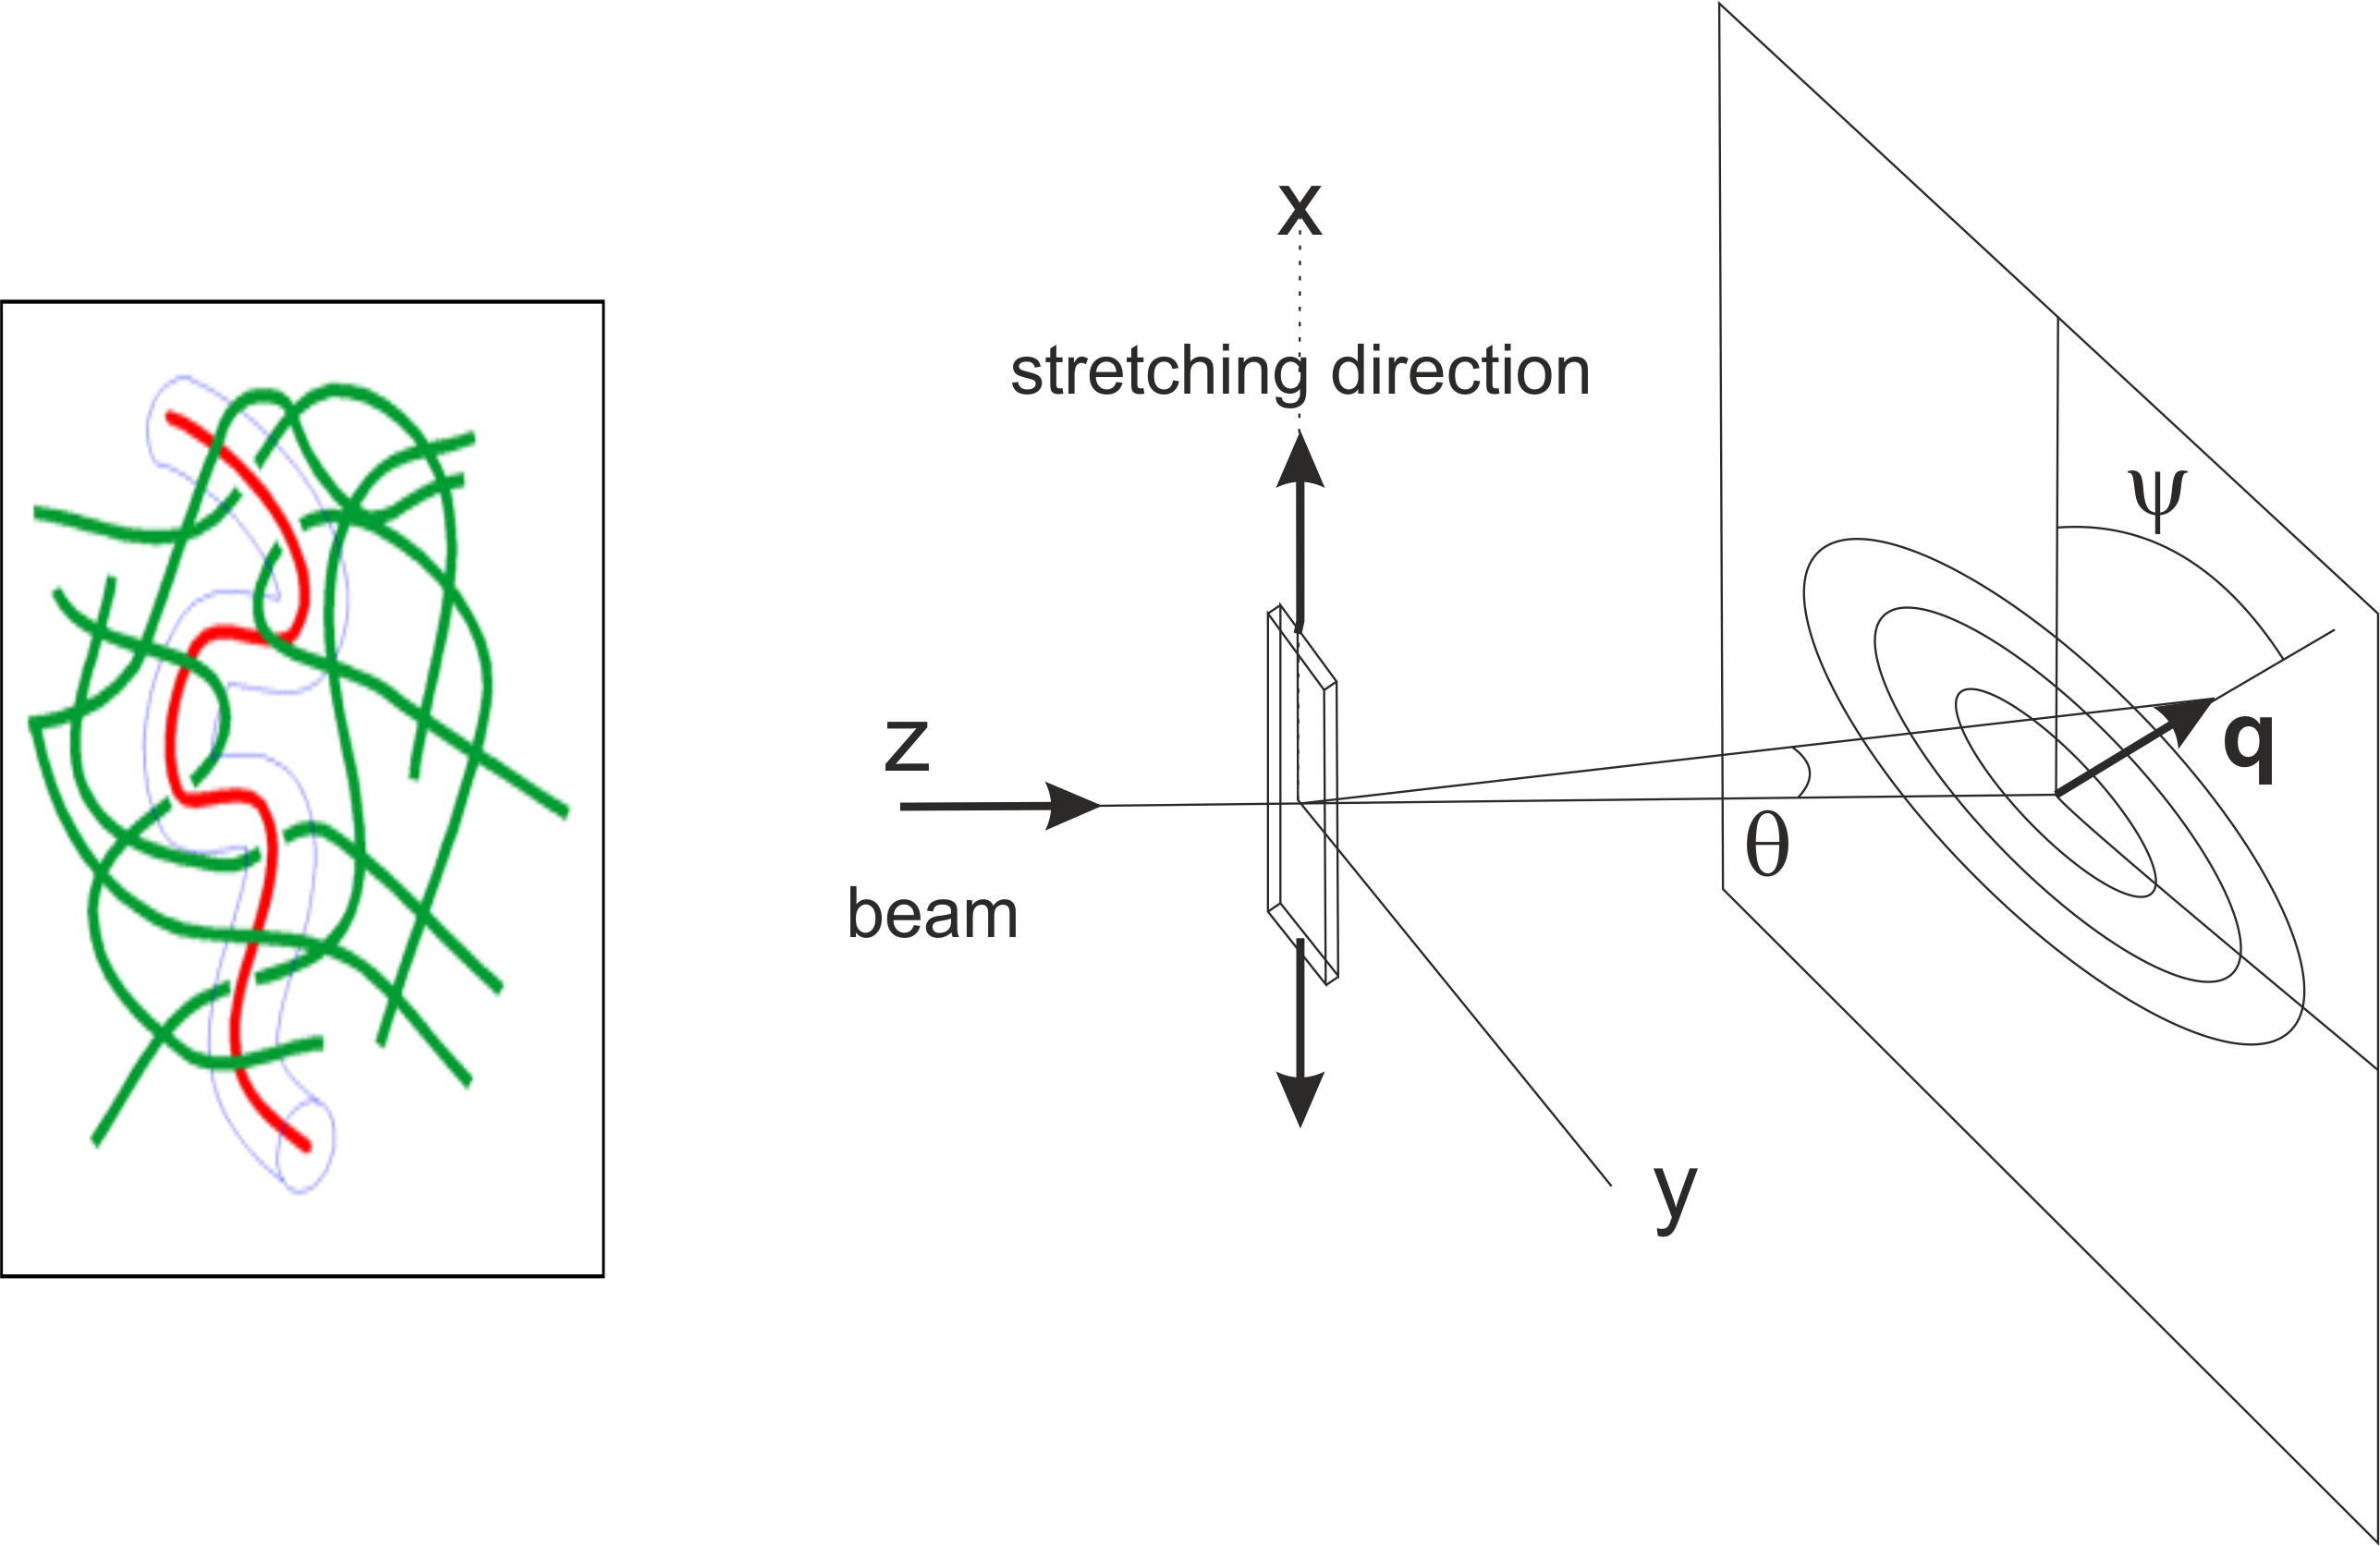
\includegraphics[width=\textwidth]{../images/form_factor/reptating_chain/reptating_chain.png}
\end{center}
\caption{Sketch of experimental setup for stretching a polymer melt.}
\label{fig:stretchpolymermelt}
\end{figure}
This model \cite{Hong1983,Noolandi1984} describes the scattering behaviour of an uniaxial deformed (stretched) Gaussian polymer chain as a function of the deformation ratio and Rouse relaxation time. The model might not include an up-to-date tube model but shows some main features of deformed polymer melts.
\newlength\breites
\settowidth\breites{$\displaystyle {}+{}$}
\begin{align}
\begin{split}
I\left(q,\frac{t}{\tau}\right)/I_0 = & \hspace{\breites}
                                        D(\alpha) + \frac{1}{6}(\alpha-\beta) \left(1+e^{-\alpha}\right) H\left(\alpha,\frac{t}{\tau}\right) \\
                                     & + \frac{1}{6}(\alpha-\beta)^2 e^{-\beta} \int_0^1 \mathrm{d}y \, y^3 e^{\beta y} \left(1+e^{-\alpha y}\right) H\left(\alpha y,\frac{t}{\tau y^2}\right)
\end{split}
\end{align}
with
\begin{align}
H\left(x,\frac{t}{\tau}\right) &= \frac{96}{\pi^2} \sum_{n = \mathrm{odd}} \frac{1}{n^2\left(n^2\pi^2+x^2\right)} e^{-n^2 \frac{t}{\tau}}
\end{align}
$D(x)$ is the Debye function $D(x) = 2\left(x - 1 + e^{-x}\right)/x^2$, $\alpha = q^2 R_g^2$, $R_g$ is the equilibrium radius of gyration
of the chain and $\tau$ is the reptation time or tube disengagement time.
Furthermore $\lambda$ is the uniaxial elongation factor, $q_\parallel$ and $q_\perp$ are respectively the components of the wave vector $q$ in directions parallel and
perpendicular to the direction of elongation which than define the parameter $\beta$ as
\begin{align}
\beta &= \left(q_\parallel^2\lambda^2+q_\perp^2/\lambda\right) R_g^2/E \\
E &= \frac{1}{2} \left\{\lambda +\frac{\mathrm{asinh}\left(\sqrt{\lambda^3-1}\right)}{\sqrt{\lambda\left(\lambda^3-1\right)}} \right\} \\
q_\parallel &= q \cos(\psi-\theta_0) \\
q_\perp &= q \sin(\psi-\theta_0)
\end{align}

\hspace{1pt}\\
\uline{Input Parameters for models \texttt{reptating chain}:}\\
\begin{description}
\item[\texttt{I0}] forward scattering $I_0$
\item[\texttt{Rg}] radius of gyration of unstretched polymer $R_g$
\item[\texttt{lambda}] stretching factor $\lambda$
\item[\texttt{t/tau}] relaxation time in units of Rouse time $t/\tau$
\item[\texttt{theta\_0}] stretching direction $\theta_0$ in the detector plane in degree
\item[\texttt{psi}] $\mathbf{q}$-direction $\psi$ in the detector plane in degree
\end{description}

\uline{Note:}
\begin{itemize}
\item The model only converges for $\lambda >1$.
\end{itemize}

\begin{figure}[htb]
\begin{center}
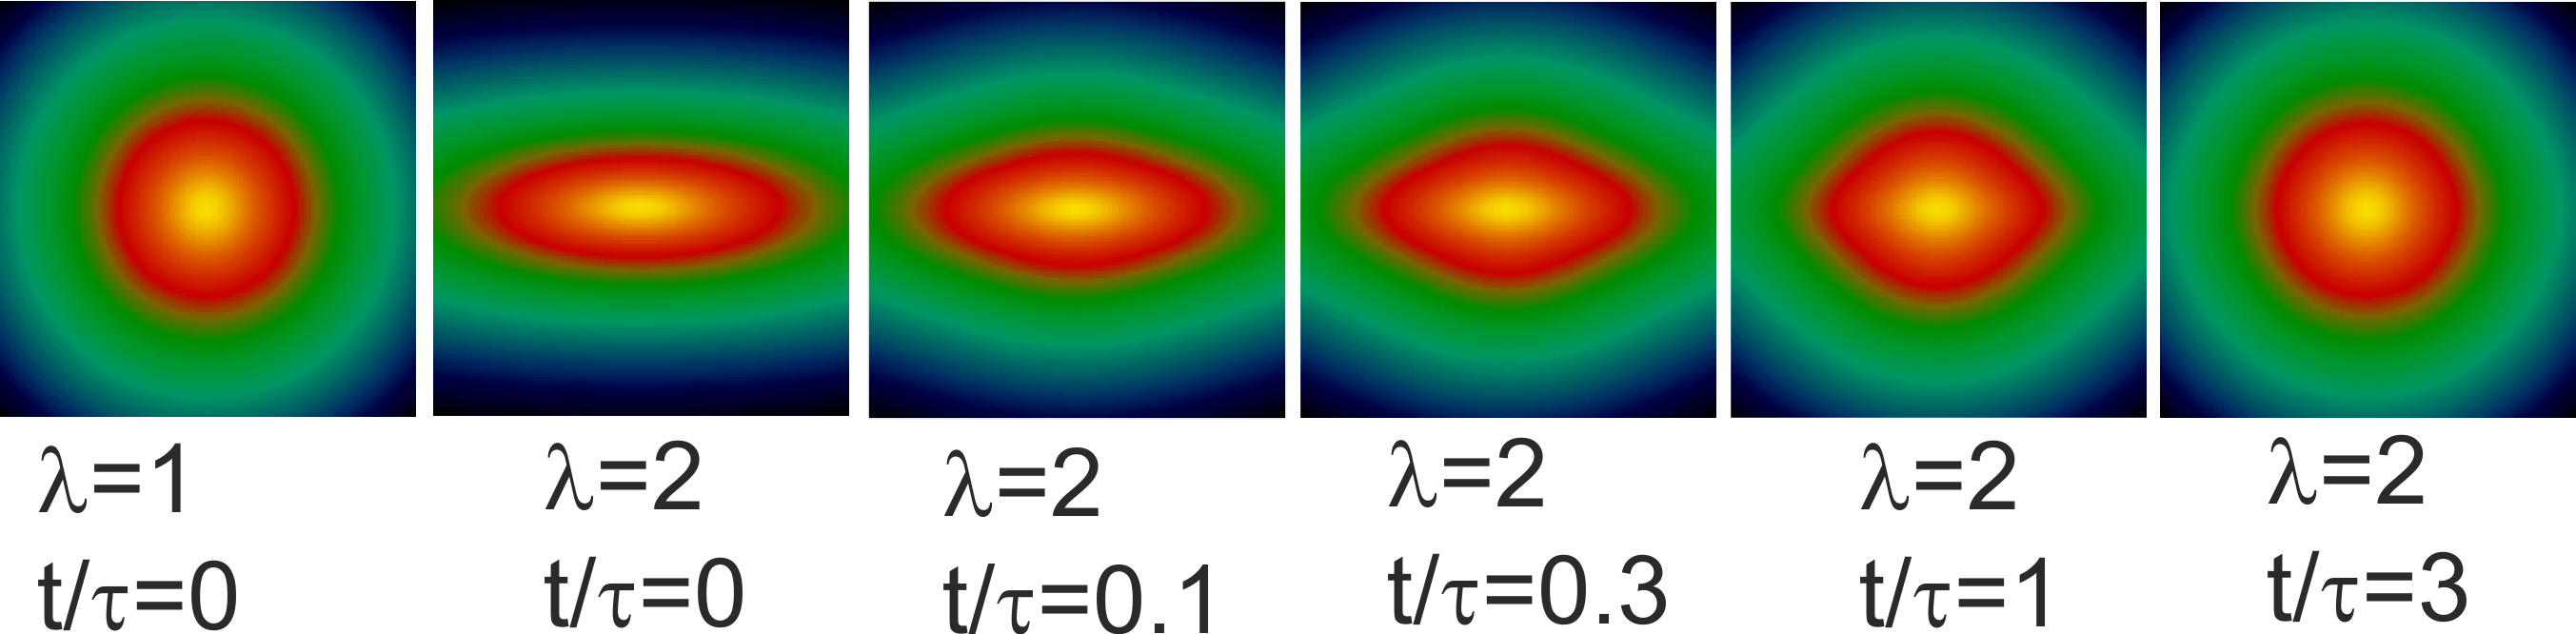
\includegraphics[width=\textwidth]{../images/form_factor/reptating_chain/lambda_2_reptating_chains.png}
\end{center}
\caption{2D scattering patterns for different relaxation times $t/\tau$ after a deformation step of $\lambda=2$}
\label{fig:IQ2Dstretchedpolymermelt}
\end{figure}

%%%%%%%%%%%%%%%%%%%%%%%%%%%%%%%%%%%%%%%%%%%%%%%%%%%%%%%%%%%%%%%%%%%%%%%%%
\newpage
\subsection{step-deformed polymer networks}
\label{sect:DeformedPolymerNetwork}
\hspace{1pt}\\
Two slightly different tube models for labeled polymer chains in a deformed network are implemented in this plugin: the original one from Warner-Edwards (WE) \cite{Warner1978} and a refined one from Heinrich-Straube-Helmis (HSH) \cite{Heinrich1988}, which have been extensively used to study uni-axial stretched polymer networks \cite{Straube1995,Mergell2001,Westermann2001,Westermann1999,Westermann1996,Read1997}.
The form factor of an uniaxial stretched polymer network with a stretching direction in the plane of the detector reads as
\begin{align}
\label{eq:SQlambda}
S(\mathbf{q},\lambda) &= \int_0^1\mathrm{d}\eta \int_0^1 \mathrm{d}\eta' \prod_{\mu} e^{-\left(Q_\mu\lambda_\mu\right)^2\abs{\eta-\eta'}-Q_\mu^2(1-\lambda_\mu^2)\xi\left\{1-\exp\left(-\frac{\abs{\eta-\eta'}}{\xi}\right)\right\}} \\
\xi &= \frac{d_\mathrm{t}^2}{2\sqrt{6}R_g^2} \\
Q_\mu &= q_\mu R_g\\
\mu  &= x,y,z \\
\mathbf{q} &= \Vek{q_x}{q_y}{q_z} = \Vek{q \cos(\psi-\delta)}{q\sin(\psi-\delta)}{0}
\end{align}
As the function of the integral kernel in eq.\ \ref{eq:SQlambda} only depends on $\abs{\eta-\eta'}$ one can transform the 2D-integral into a 1D-integral by using the identity
\begin{align}
\label{eq:2D1D_int_identity}
\int_0^1\mathrm{d}\eta \int_0^1 \mathrm{d}\eta' \: K\left(\abs{\eta-\eta'}\right) &= 2 \int_0^1 (1-x)K(x)\: \mathrm{d}x
\end{align}
The difference between the WE-model and the HSH-model is how the deformed tube diameter $d_\mathrm{t}$ is calculated. In case of the WE-model the projection $d_\mu$ of $d_t$ onto the Cartesian axis are used, whereas the HSH-model uses an effective angle dependent diameter $d_\phi$.
\begin{align}
\mbox{(WE-model): } d_\mathrm{t} &= d_\mu^2 = d_0^2\lambda_\mu^{2\nu} \\
\mbox{(HSH-model): } d_\mathrm{t} &= d_\phi^2 = d_0^2\lambda_\phi^{2\nu}
\end{align}
If we assume an elongation ratio of $\lambda$ in the $x$-direction
\begin{align}
  \lambda_x &=\lambda_{\|}=\lambda, \quad \lambda_y=\lambda_z=\lambda_\perp=\frac{1}{\sqrt{\lambda}} \\
  \lambda_\phi^2 &= \lambda_{\|}^2 \cos^2(\psi-\delta)+\lambda_\perp^2\sin^2(\psi-\delta)
\end{align}
where $R_g$ the radius of gyration of the un-deformed polymer network $\lambda_\mu$ is the macroscopic stretch ratio in this Cartesian direction and the exponent $\nu$ is predicted to take a value of $1/2$ in the case of networks \cite{Straube1995,Read2004}.  Nevertheless $\nu$ is kept as a fit parameter in this plug-in function.
\begin{multline}
\label{eq:SQ_WE_HSH}
%\begin{split}
S^\mathrm{WE}(\mathbf{q},R_g,\lambda,\nu,d_0) = \\ 2\int_0^1\mathrm{d}x\: (1-x) e^{\left(\sum_{\mu} -Q_\mu^2\lambda_\mu^2 x-
(1-\lambda_\mu^2)Q_\mu^2\xi_\mu\left\{1-e^{\left(-\frac{x}{\xi_\mu}\right)}\right\}\right)}
\end{multline}
\begin{multline}
S^\mathrm{HSH}(\mathbf{q},R_g,\lambda,\nu,d_0) = \\ 2\int_0^1\mathrm{d}x\: (1-x) e^{\left(\sum_{\mu} -Q_\mu^2\lambda_\mu^2 x- % \\ &\qquad \qquad
 (1-\lambda_\mu^2)Q_\mu^2\xi_\phi\left\{1-e^{\left(-\frac{x}{\xi_\phi}\right)}\right\}\right)}
\end{multline}
with
\begin{align}
  \xi_\mu =& \frac{d_\mu^2}{2\sqrt{6}R_g^2} \\
  \xi_\phi =& \frac{d_\phi^2}{2\sqrt{6}R_g^2}
\end{align}
In a work of \cite{Ariane2004} an additional retraction coefficient $\gamma(t)$ has been included so that the final equation for the HSH model reads as
\begin{multline}
\label{eq:SQ_HSH_retraction}
S^\mathrm{HSH}(\mathbf{q},R_g,\lambda,\nu,\gamma,d_0) =  2\int_0^1\mathrm{d}x\: (1-x) \exp\Bigg(\sum_{\mu} Q_\mu^2\left[-\lambda_\mu^2\frac{x}{\gamma(t)}- \right. \\
\left. \xi_\phi\left\{1-e^{\left(-\frac{x}{\xi_\phi\gamma(t)}\right)}\right\} +\lambda_\mu^2\xi_\phi\left\{1-e^{\left(-\frac{x}{\xi_\phi}\right)}\right\} \right]\Bigg)
\end{multline}
The retraction coefficient is for short times $\gamma(t=0)=1$ and becomes larger for increasing relaxation times $\gamma(t>0)>1$.

\begin{figure}[htb]
\begin{center}
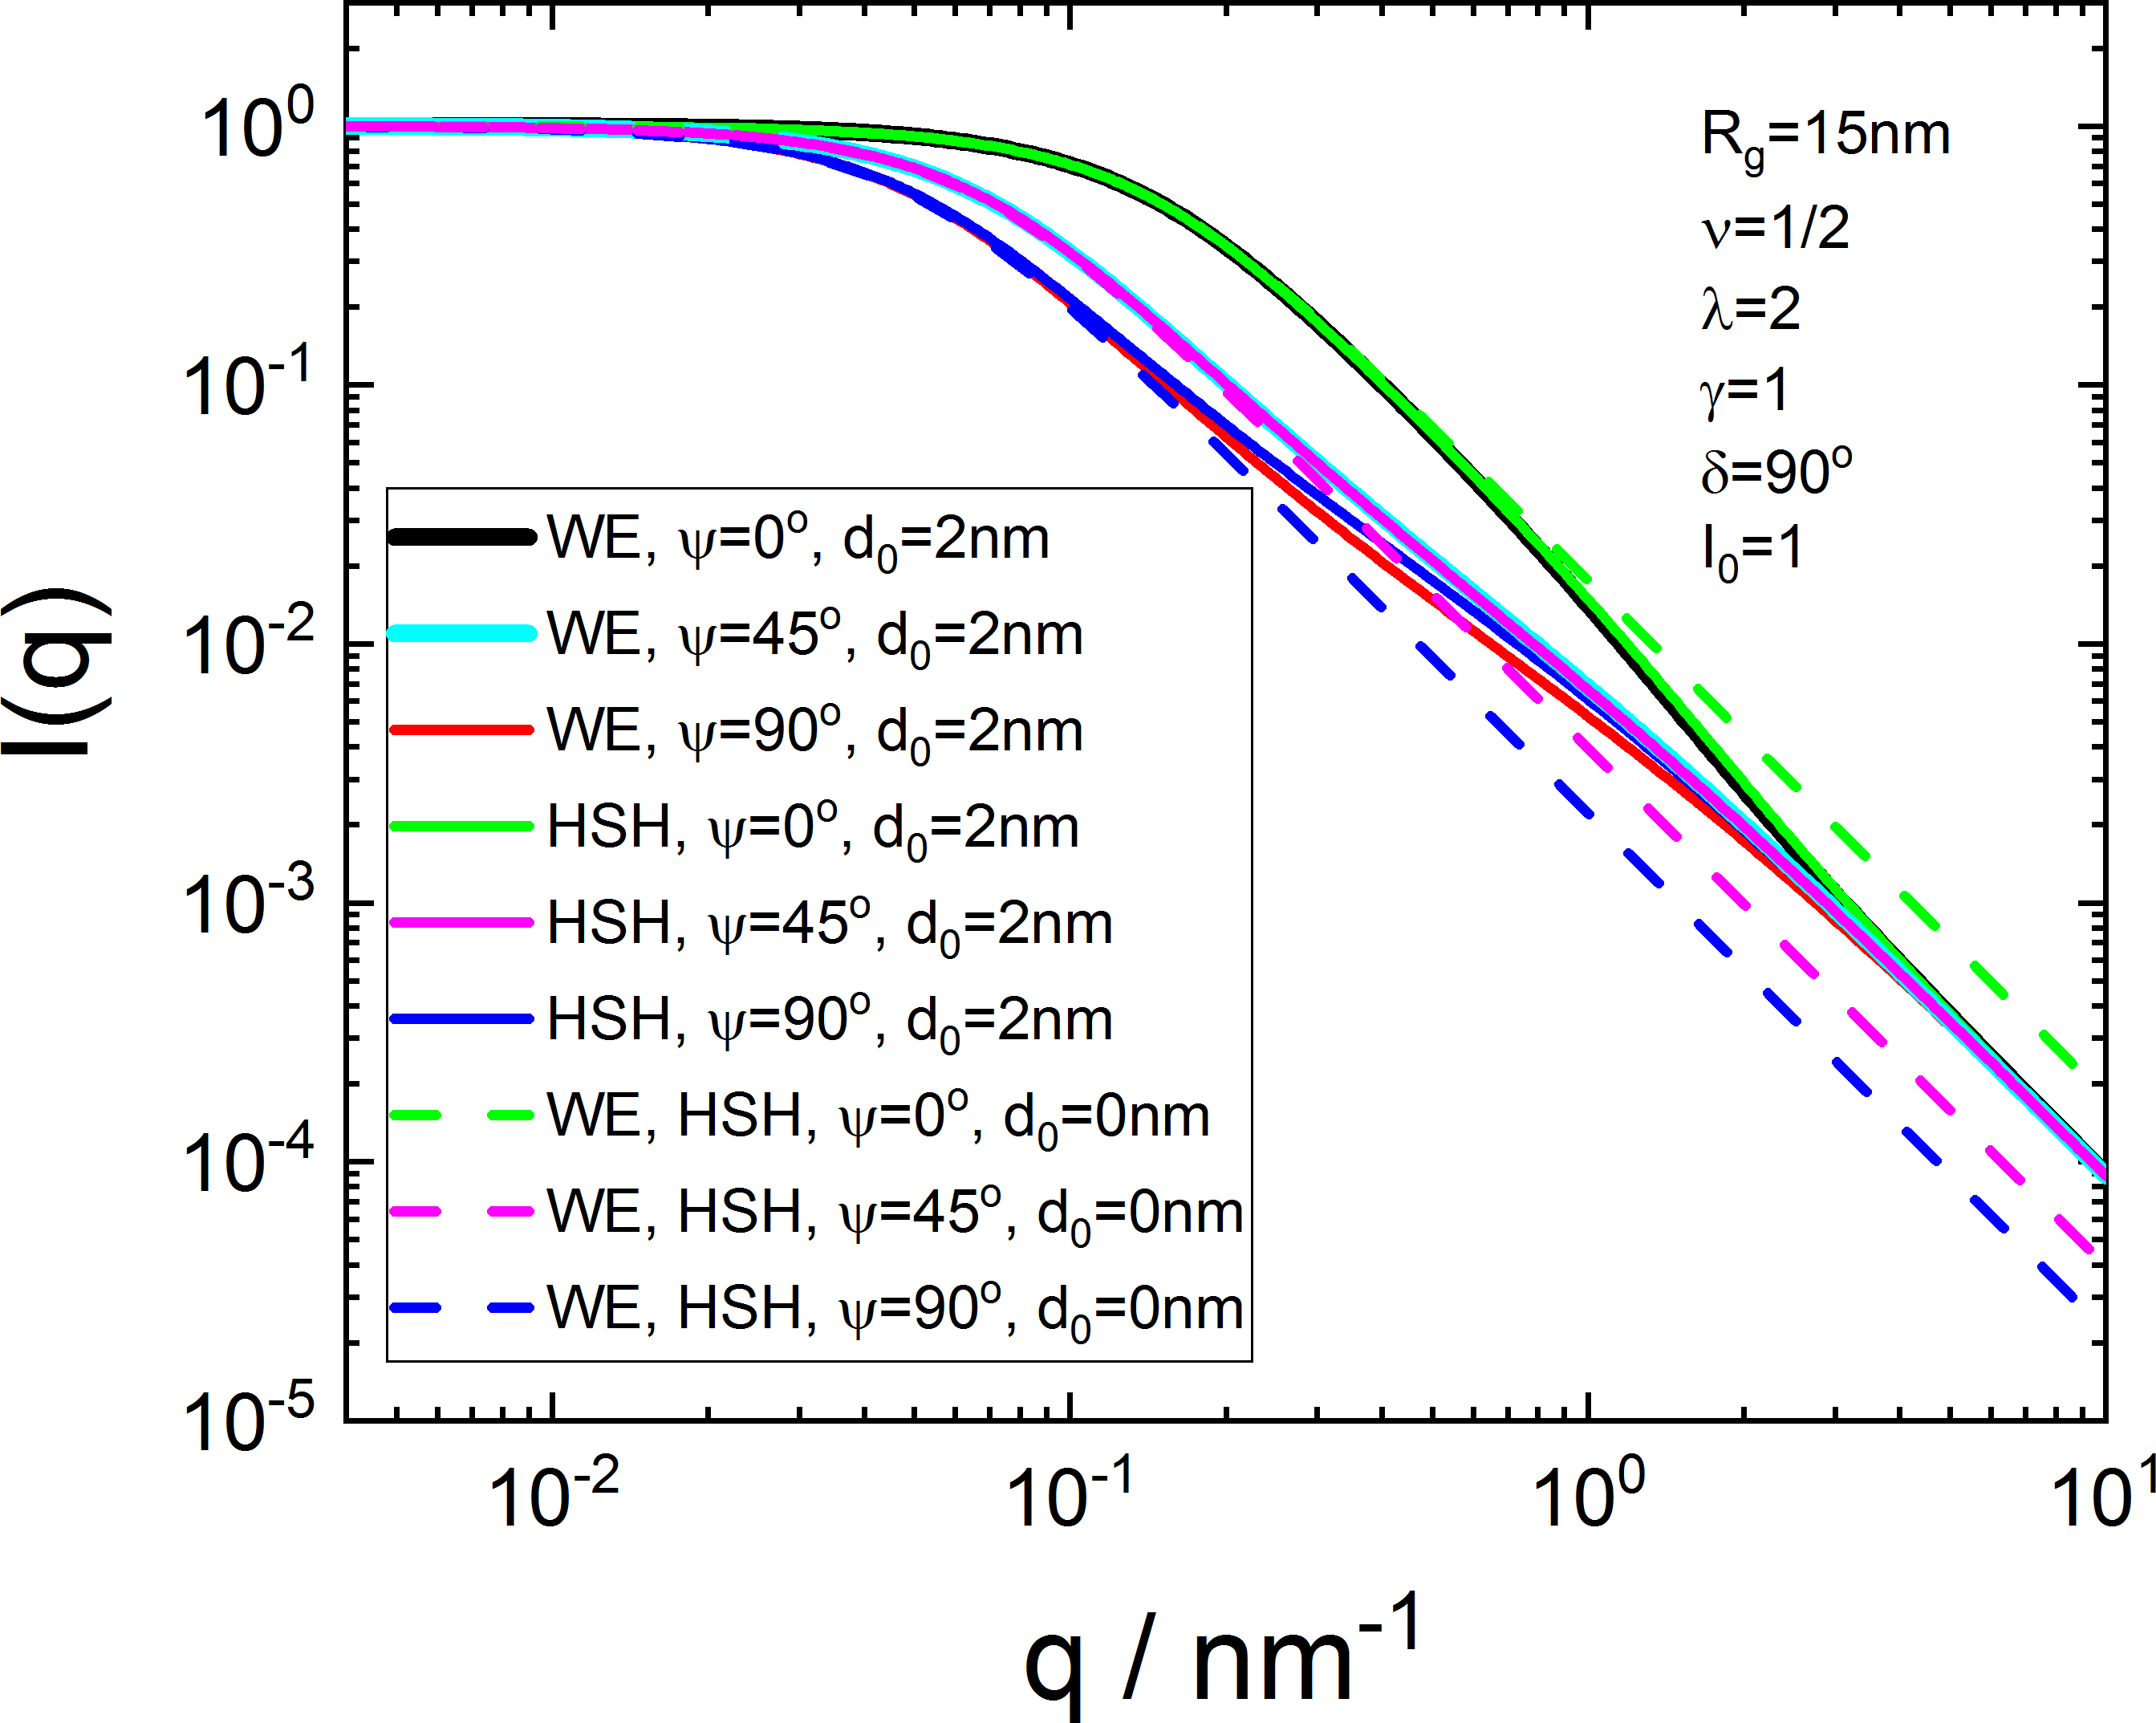
\includegraphics[width=0.7\textwidth]{../images/form_factor/deformed_sheared/deformed_polymer_network_I(sector).png}
\end{center}
\caption{sector averaged scattering curves of the Warner-Edwards and Heinrich-Straube-Helmis model of step-deformed polymer networks for tube diameters $d_0$ of 2nm and zero nm}
\label{fig:I(sector)polymernetwork}
\end{figure}

\hspace{1pt}\\
\uline{Input Parameters for models \texttt{WE: deformed polym. netw.}:}\\
\begin{description}
\item[\texttt{I0}] forward scattering $I_0$
\item[\texttt{Rg}] radius of gyration of unstretched polymer $R_g$
\item[\texttt{d0}] equilibrium tube diameter $d_0$
\item[\texttt{nu}] exponent ($\nu=1/2$, $\nu=1$:affine deformation)
\item[\texttt{lambda}] deformation ratio $\lambda$ along deformation axis
\item[\texttt{dummy}] not used
\item[\texttt{psi}] direction $\psi$ of the scattering vector $\mathbf{q}$ in the detector plane in degree
\item[\texttt{delta}] stretching direction in the detector plane $\delta$ in degree
\end{description}

\hspace{1pt}\\
\uline{Input Parameters for models \texttt{HSH: deformed polym. netw.}:}\\
\begin{description}
\item[\texttt{I0}] forward scattering $I_0$
\item[\texttt{Rg}] radius of gyration of unstretched polymer $R_g$
\item[\texttt{d0}] equilibrium tube diameter $d_0$
\item[\texttt{nu}] exponent ($\nu=1/2$, $\nu=1$:affine deformation)
\item[\texttt{lambda}] deformation ratio $\lambda$ along deformation axis

\item[\texttt{gamma}] retraction coefficient ($1 < \gamma \lesssim 2$)
\item[\texttt{psi}] direction $\psi$ of the scattering vector $\mathbf{q}$ in the detector plane in degree
\item[\texttt{delta}] stretching direction in the detector plane $\delta$ in degree
\end{description}

\uline{Note:}
\begin{itemize}
\item for large $q$-values the integration routines might fail to converge.
\end{itemize}

\begin{figure}[htb]
\begin{center}
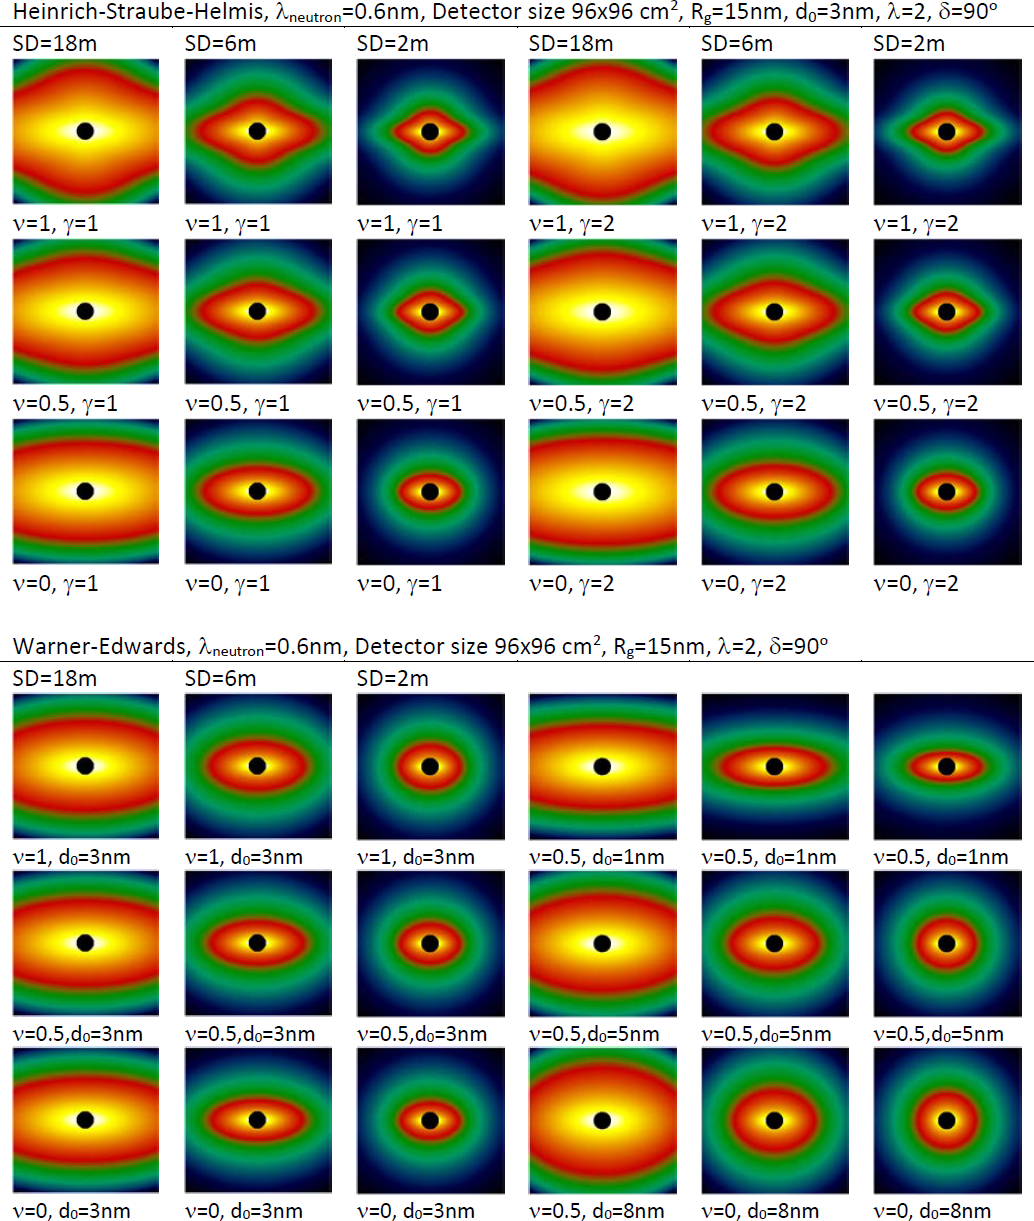
\includegraphics[width=0.7\textwidth]{../images/form_factor/deformed_sheared/deformed_polymer_network.png}
\end{center}
\caption{2D scattering patterns of the Warner-Edwards and Heinrich-Straube-Helmis model of step-deformed polymer networks}
\label{fig:IQ2Dpolymernetwork}
\end{figure}


%%%%%%%%%%%%%%%%%%%%%%%%%%%%%%%%%%%%%%%%%%%%%%%%%%%%%%%%%%%%%%%%%%%%%%%%%
\newpage
\subsection{polymer under shear flow}~\\
\label{sect:PolymerShearFlow}

This plugin is implemented for a certain experimental setup of a quenched shear sample using two different configuration. The sample has a disc shape of a few mm in diameter and was sheared in a cone-plate geometry. Therefore, the vorticity, flow and gradient direction are well described in a cylindrical coordinate system $\mathbf{e}_\rho$, $\mathbf{e}_\varphi$, and $\mathbf{e}_z$. The normal of the disc represents the gradient direction of the sheared sample $\mathbf{e}_z=\mathbf{e}_g$. The radial direction $\mathbf{e}_\rho=\mathbf{e}_v$ represents the vorticity direction and the azimuth direction the flow direction $\mathbf{e}_\varphi=\mathbf{e}_f$.
\begin{enumerate}
\item In one experimental geometry the normal $\mathbf{e}_g$ (gradient direction) of the disc shaped sample is parallel to the incoming neutron beam $\mathbf{e}_n$. To separate the deformation in flow and vorticity direction apertures with a sector shape and two opposite openings of 45 degree each as marked in the image below are used. In this geometry the scattering in this setup is sensitive to in vorticity and flow direction only.\\[3mm]

    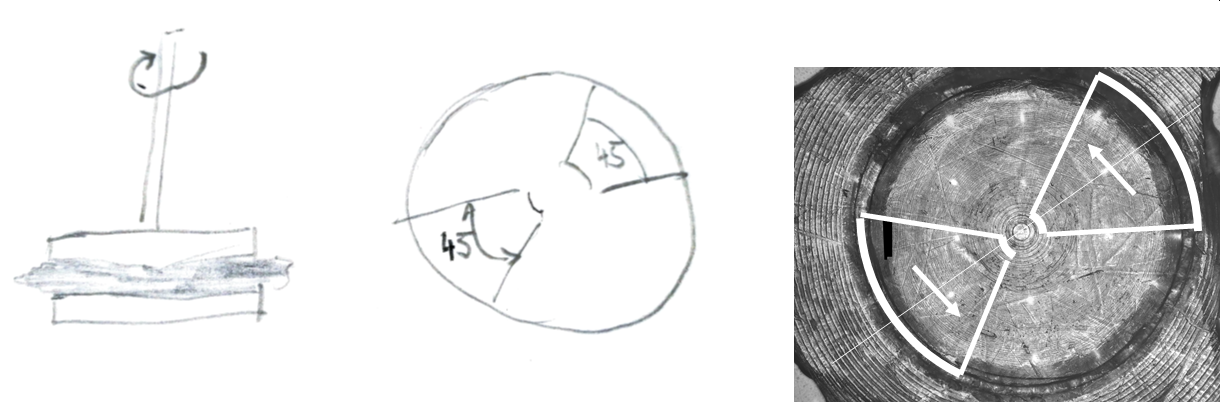
\includegraphics[width=0.85\textwidth]{../images/form_factor/deformed_sheared/sample1.png} \\

\item In a second setup a fully opened circular aperture (no sectors) of the same diameter as the sample is mounted and turned with the sample around the vertical axis by an angle $\theta_0$. Depending on the turning angle $\theta_0$ the horizontal detector direction probes a mixture of the averaged flow/vorticity contribution and the scattering in gradient direction. The contributions depend on the projection of the scattering vector onto the plane of the disc and to the normal of the disc being the gradient direction \\[3mm]

   \noindent  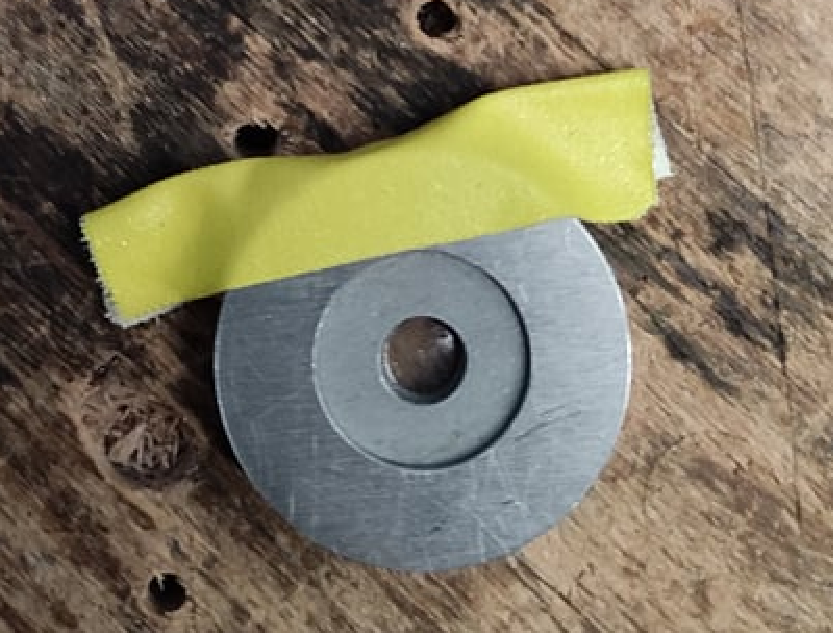
\includegraphics[width=0.377\textwidth]{../images/form_factor/deformed_sheared/mag_tilted_sample.pdf} ~
    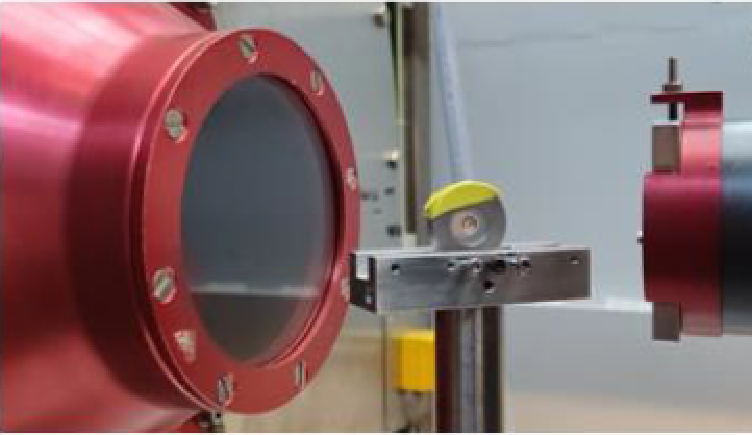
\includegraphics[width=0.5\textwidth]{../images/form_factor/deformed_sheared/tilted_sample.pdf} \\

\end{enumerate}

The form factors describing linear polymers under shear flow has been taken from \cite{Korolkovas2019}.
In the original paper it is assumed that the shear-vorticity plane is the same than the detector plane. We slightly extend it here to any orientation defined by proper Euler angles.

The form factor of polymers is deduced from the mean squared distance (MSD) $\langle(\mathbf{q}\cdot\mathbf{r}_{nm})^2\rangle/2$ within a polymer chain and is given by a double integral
\begin{align}
  P(\mathbf{q}) & = \frac{1}{N^2}\int_0^N\mathrm{d}n\int_0^N\mathrm{d}m\: \exp\left(-\frac{\langle(\mathbf{q}\cdot\mathbf{r}_{nm})^2\rangle}{2}\right)
\end{align}
If the mean squared distance function (MSD) $\langle(\mathbf{q}\cdot\mathbf{r}_{nm})\rangle/2$ can be written as a function of $\nu=\left|n-m\right|/N$, one can replace the double integral by a single integral.
\begin{align} \label{eq:IQ_MSD}
 P(\mathbf{q}) & = 2\int_0^1 (1-\nu) \exp\left(-\frac{\langle(\mathbf{q}\cdot\mathbf{r}_{nm})^2\rangle}{2}\right) \mathrm{d}\nu
\end{align}
Here the polymer consists if $N$ flexible units where $\mathbf{r}_{nm}$ is the vectorial distance between the centers of the $n^\mathrm{th}$ and $m^\mathrm{th}$ monomer unit.
The scattering vector in the laboratory system is
\begin{align}
\mathbf{q} &= q
\left(
    \begin{array}{c}
        \cos(\phi) \\
        \sin(\phi) \\
        0 \\
    \end{array}
\right)
\end{align}
The vectorial distance between  $\mathbf{r}_{nm}$ in defined here in the coordination system of the applied flow
\begin{align}
\mathbf{r}_{nm} &= x_{v,nm} \mathbf{e}_{v,nm} + z_{f,nm} \mathbf{e}_{f} + y_{g,nm} \mathbf{e}_{g}
\end{align}
The averages to be taken are then
\begin{align}
\begin{split} \label{MSDfull}
 \langle(\mathbf{q}\cdot\mathbf{r}_{nm})^2\rangle  & = q_v^2 \langle x_{v,nm}^2\rangle + q_f^2 \langle z_{f,nm}^2\rangle + q_g^2 \langle y_{g,nm}^2\rangle + \\
 & 2q_v q_f \langle x_{v,nm} z_{f,nm}\rangle + 2q_v q_g \langle x_{v,nm} y_{g,nm}\rangle + 2q_fq_g \langle z_{f,nm}y_{g,nm}\rangle
 \end{split}
\end{align}
with
\begin{align}
  q_g &= \mathbf{q}\cdot \mathbf{e}_g \label{eq:eg} \\
  q_f &= \mathbf{q}\cdot \mathbf{e}_f \label{eq:ef} \\
  q_v &= \mathbf{q}\cdot \mathbf{e}_v \label{eq:ev}
\end{align}
The unit vectors $\mathbf{e}_g$, $\mathbf{e}_f$, and $\mathbf{e}_v$ are determined by the sample orientation and will be defined later on. In the following it is assumed, that the mixed terms in eq.\ \ref{MSDfull} are negligible (this is exactly true for an undeformed linear polymer in equilibrium) and only the squared terms (which are symmetric for the undeformed polymer) contribute to the mean squared internal distance so that eq.\ \ref{MSDfull} simplifies to
\begin{align} \label{MSDused}
 \langle(\mathbf{q}\cdot\mathbf{r}_{nm})^2\rangle  & = q_v^2 \langle x_{v,nm}^2\rangle + q_f^2 \langle z_{f,nm}^2\rangle + q_g^2 \langle y_{g,nm}^2\rangle
 \end{align}
An undeformed linear polymer in equilibrium has an exact solution for the MSD
\begin{align}\label{MSDequilibrium}
  \langle(\mathbf{q}\cdot\mathbf{r}_{nm})^2\rangle/2 & = a |n-m|/N
\end{align}
and is a straight line with a slope $a=q^2R_g^2=q^2N\lambda^2/6$ , where $\lambda$ is the
Kuhn length and $R_g$ the equilibrium radius of gyration. $N$ is the number of Kuhn segments of a single polymer chain. This leads to the scattering function
\begin{align}
  P_\mathrm{lin,iso}(\mathbf{q}) & = \frac{2\left(e^{-a}-1+a\right)}{a^2}
\end{align}

\subsection{linear polymer under shear flow}~\\
\label{sect:LinearPolymerShearFlow}

\begin{figure}[htb]
  \centering
  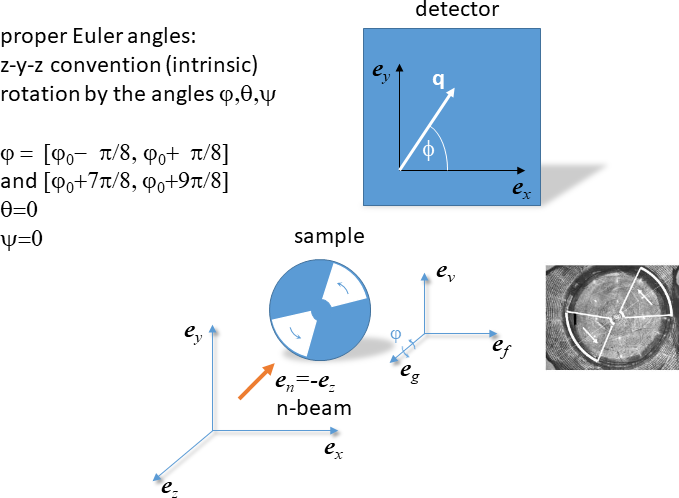
\includegraphics[width=.8\textwidth]{../images/form_factor/deformed_sheared/Euler_case1.png}
  \caption{used coordination axis and Euler angles for case 1}\label{fig:EulerCase1}
\end{figure}

\begin{figure}[htb]
  \centering
  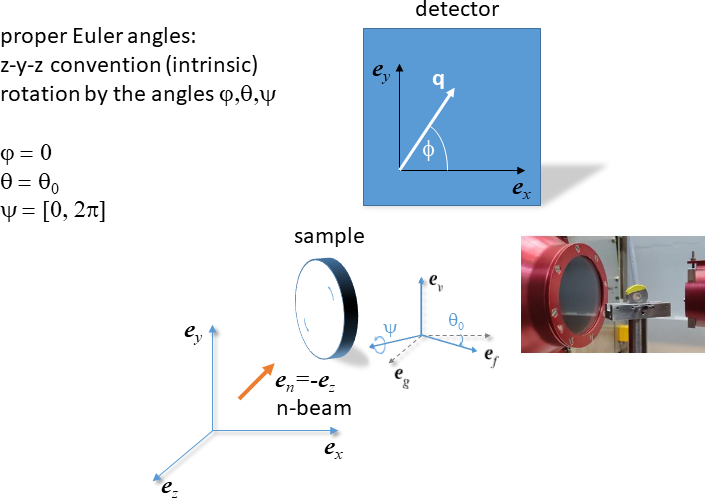
\includegraphics[width=.9\textwidth]{../images/form_factor/deformed_sheared/Euler_case2.png}
  \caption{used coordination axis and Euler angles for case 2}\label{fig:EulerCase2}
\end{figure}


For a sheared linear polymer the mean squared distance MSD in the flow, vorticity and gradient direction has been approximated in \cite{Korolkovas2019} by a piecewise linear approximation and with a limitation to just two segments.
The approximation of the MSD by a series of two straight lines reads as
\begin{align}\label{eq:2straightlines}
\frac{\langle(\mathbf{q}\cdot\mathbf{r}_{nm})^2\rangle}{2}  &=
\begin{cases}
  b|n-m|/N, & \mbox{if } |n-m|/N<f \\
  c|n-m|/N+(b-c)f, & \mbox{otherwise}.
\end{cases}
\end{align}
with $f\in (0,1)$. Depending on the orientation of the sample one probes in a certain scattering direction the contribution of the different projections of the shear axis on $\mathbf{q}$ (only diagonal contributions are assumed). The slopes are give by
\begin{align}
  b &= R_g^2 \left[\alpha^2q_f^2+\beta^2 q_v^2+\gamma^2 q_g^2\right] \label{eq:slope_b} \\
  c &= R_g^2 \left[A^2q_f^2+B^2 q_v^2+\mathit{\Gamma}^2 q_g^2\right] \label{eq:slope_c}
\end{align}
The form factor for such a slope in the MSD is given by
\begin{multline}\label{eq:slopes_bc_PQ}
P_\mathrm{lin,2}(q,R_g,\alpha,\beta,\gamma,A,B,\mathit{\Gamma}) = \frac{2}{b^2}\Bigg(b-1+\exp\left(-fb\right) \times \\
    \left\{1+\left[\frac{b^2}{c^2}-1\right]\exp\left((f-1)c\right)+(1-f)\frac{b(b-c)}{c}\right\}\Bigg)
\end{multline}
with a radius of gyration $R_{g,\mathrm{lin}}$
\begin{align}\label{eq:Rglin_straight}
  R_{g,\mathrm{lin,2}} &= R_{g}\sqrt{c+(b-c)\left(3f-3f^2+f^3\right)}
\end{align}


The parametrization above does not automatically preserve the contour length of the polymer.

The last missing part is to define the orientation of the three shear vectors to get the projection $q_g$,$q_f$, $q_v$ of of them on $\mathbf{q}$ (eqs.\ \ref{eq:eg}-\ref{eq:ev}) as they are needed to calculate the slopes $b$ and $c$ in eq.\ \ref{eq:slope_b} and \ref{eq:slope_c}.

To values for these vectors are obtained by rotation of the laboratory axis into the shear coordination system. This can be done by using Euler angles. For the chosen coordination system proper Euler angles using $z$-$y$-$z$ convention using the angles $\varphi$, $\theta$, $\psi$ are well suited \cite{reference.wolfram_2022_eulerangles}. Lets $\mathbf{M}_{\varphi,\theta,\psi}$ be the rotation matrix, then the shear vector are given by
\begin{align}\label{eq:rotated_shear_vectors}
  \mathbf{e}_f &= \mathbf{M}_{\varphi,\theta,\psi} \; \mathbf{e}_x \\
  \mathbf{e}_v &= \mathbf{M}_{\varphi,\theta,\psi} \; \mathbf{e}_y \\
  \mathbf{e}_g &= \mathbf{M}_{\varphi,\theta,\psi} \; \mathbf{e}_z
\end{align}
where $\mathbf{e}_x=(1,0,0)^T$, $\mathbf{e}_y=(0,1,0)^T$, and $\mathbf{e}_z=(0,0,1)^T$. The Euler matrix $\mathbf{M}_{\varphi,\theta,\psi}$ using $z$-$y$-$z$ convention reads as
\begin{align}
\mathbf{M}_{\varphi,\theta,\psi} &=
\left(
\begin{array}{ccc}
 c_{\theta } c_{\psi } c_{\varphi }-s_{\psi } s_{\varphi } & -c_{\theta } c_{\varphi } s_{\psi }-c_{\psi } s_{\varphi } & c_{\varphi } s_{\theta } \\
 c_{\theta } c_{\psi } s_{\varphi }+c_{\varphi } s_{\psi } & c_{\psi } c_{\varphi }-c_{\theta } s_{\psi } s_{\varphi } & s_{\theta } s_{\varphi } \\
 -c_{\psi } s_{\theta } & s_{\theta } s_{\psi } & c_{\theta } \\
\end{array}
\right)
\end{align}
with $c_x=\cos(x)$ and $s_x=\sin(x)$.
By defining the shear vectors via a rotation matrix of the cartesian unit vectors the form factor now also depends on the Euler angles so that it becomes a function of $P(q,R_g,\alpha,\beta,\gamma,A,B,\mathit{\Gamma},\varphi,\theta,\psi)$.,

At least for the cases 1 and 2 mentioned at the beginning this allows to simply integrate over the orientations of the shear vectors defined by the turning angle of the sample and apertures shapes used.

For the case 1 the axis are shown in fig.\ \ref{fig:EulerCase1}. In this setup the sample is already placed with its gradient direction parallel to the beam. The aperture in front of the sample has only aperture opening of sector with for example $\Delta\varphi=45^\circ=\pi/4$. As the two sectors are not aligned to the $x$-axis but turned by $\varphi_0$ the aperture smearing can be included by
\begin{align}\label{eq:case1}
  I_{\mathrm{lin},2,\mathrm{a}}(\mathbf{q}) & = 2\int_{\varphi_0-\Delta\varphi/2}^{\varphi_0+\Delta\varphi/2} P_\mathrm{lin,2}(q,R_g,\alpha,\beta,\gamma,A,B,\mathit{\Gamma},\varphi,\theta=0,\psi=0) \;\mathrm{d}\varphi
\end{align}
As the scattering intensity is symmetric and the second sector is turned by $\pi$ it produces the same scattering contribution as the first one.

Also the second case, where the sample has been rotated in the beam by an angle $\theta_0$ can easily be described. In that case the aperture in front of the sample has a full circular opening as shown in fig.\ \ref{fig:EulerCase2}, but is turned in the beam around the vertical $y$-axis by $\theta_0$. Therefore the scattering intensity for case 2 is given by
\begin{align}\label{eq:case1}
  I_{\mathrm{lin},2,\mathrm{b}}(\mathbf{q}) & = \int_{0}^{2\pi} P_\mathrm{lin,2}(q,R_g,\alpha,\beta,\gamma,A,B,\mathit{\Gamma},\varphi=0,\theta=\theta_0,\psi) \;\mathrm{d}\psi
\end{align}
The intensity for $\theta=0$ should not depend on the azimuthal angle $\psi$. However, in some case a certain anisotropy has been seen like shown in fig.\  \ref{fig:offcentered}.
\begin{figure}[htb]
  \centering
  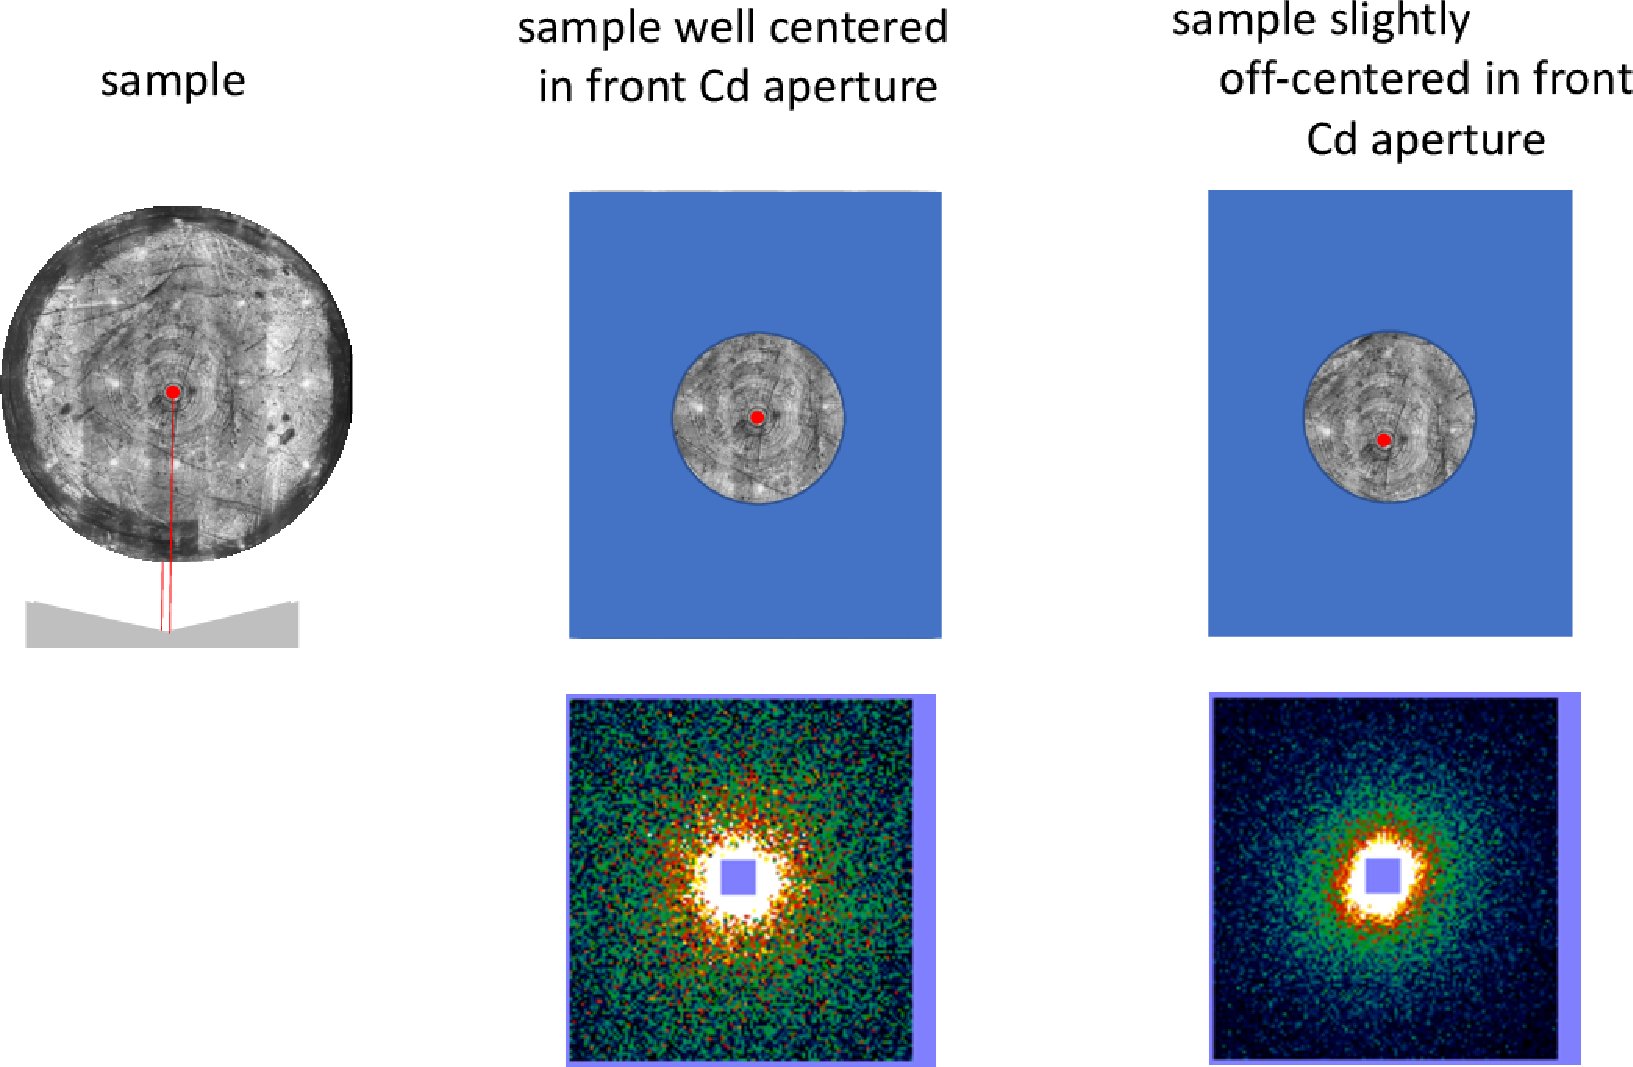
\includegraphics[width=.66\textwidth]{../images/form_factor/deformed_sheared/offcentered.pdf}
  \caption{effect of off-centered samples in front of aperture}
  \label{fig:offcentered}
\end{figure}

To account for a possible off-centered sample the azimuthal integration would need to be done including a certain orientation probability distribution $p(\psi,\psi_0,S_2,S_4)$ of the flow direction.
\begin{align}\label{eq:case1offcentered}
  I_2(\mathbf{q}) & = \frac{1}{2\pi}\int_{0}^{2\pi}  f(\psi-\psi_0,S_2,S_4) \; P_\mathrm{lin}(q,R_g,\alpha,\beta,\gamma,A,B,\mathit{\Gamma},\varphi=0,\theta,\psi) \;\mathrm{d}\psi
\end{align}
The orientation distribution function is simply described in terms of Legendre polynomials.
\begin{align}
f(\psi) &= \sum_l c_l P_l(\cos\psi) = \sum_l \frac{2l+1}{2} S_l P_l(\cos\psi)
\end{align}
with the first three Legendre polynomials defined by
\begin{subequations}
\begin{align}
P_0(\cos\psi) &= 1\\
P_1(\cos\psi) &= \cos\psi\ \\
P_2(\cos\psi) &= \frac{1}{2}\left(3\cos^2\psi-1\right)
\end{align}
\end{subequations}
As the orientation distribution was assumed to be symmetric to $\psi_0$ only odd terms have been considered. In practice the off centered alignment could be sufficiently good corrected for using just the $P_0(\cos\psi)$ and $P_2(\cos\psi)$ with $c_0=1$ and $c_2$ and $\psi_0$ being fit parameters.

\begin{itemize}
\item  a semi-empirical 3-parameter formula $(B_x,B_y,\xi)$ to have a similar shape then the piecewise linear MSD function above.
    \begin{multline}
    \frac{\langle(\mathbf{q}\cdot\mathbf{r}_{nm})^2\rangle}{2} =\left(qR_g\right)^2 \times \\
    \left\{
      \abs{\frac{n-m}{N}} + \left[B_x^2\cos^2(\psi-\phi_0)-B_y^2\sin^2(\psi-\phi_0)\right]\abs{\frac{n-m}{N}}^\xi
    \right\}
    \end{multline}
    To get the same endpoints than the piecewise linear MSD function the amplitudes should be $B_x=\sqrt{\nu\alpha^2+(1-\nu)\gamma^2}$ and $B_y=\sqrt{\nu\beta^2+(1-\nu)\delta^2}$.
    After making use of the identity \ref{eq:2D1D_int_identity} the scattering intensity is than given by
    \begin{multline}
      P(\mathbf{q}) = 2 \int_0^1 (1-x) \exp\Bigg( \left(qR_g\right)^2\\
      \left(
      x + \left(B_x^2q^2\cos^2(\psi-\phi_0)+B_y^2q^2\sin^2(\psi-\phi_0)\right)x^\xi
      \right)\Bigg)
    \end{multline}
\item by applying the Rouse model \cite{Korolkovas2019} the MSD which reads as
    \begin{multline}\label{eq:MSDlinearShearFlow}
    \frac{\langle(\mathbf{q}\cdot\mathbf{r}_{nm})^2\rangle}{2} = \left(qR_g\right)^2 \times \\ \left[ x+\frac{\left(\cos(\psi-\phi_0)\pi^2\operatorname{Wi}_\mathrm{lin}\right)^2}{180} x^2\left(1+x-x^2/4-2x^3+x^4\right) \right]
    \end{multline}
    with $x=\abs{\frac{n-m}{N}}$ and the Weissenberg number $\operatorname{Wi}_\mathrm{lin}=\tau_1\dot{\gamma}$.
\end{itemize}

\subsection{Ring polymer under shear flow}~\\
\label{sect:RingPolymerShearFlow}

Ring polymers under shear flow also can be described using the Rouse model \cite{Tsolou2010,Stephanou2019} similarly to eq.\ \ref{eq:MSDlinearShearFlow}. The mean square displacement then reads as
\begin{align}\label{eq:MSDringShearFlow}
\frac{\langle(\mathbf{q}\cdot\mathbf{r}_{nm})^2\rangle}{2} &= 2\left(qR_{g,\mathrm{ring}}\right)^2
\left[ \mu+\frac{\left(\cos(\psi-\phi_0)\pi^2\operatorname{Wi}_\mathrm{ring}\right)^2}{1440} \left(\mu^2+2\mu^3\right) \right]
\end{align}
with $\mu=x(1-x)$, $x=\abs{\frac{n-m}{N}}$, $\operatorname{Wi}_\mathrm{ring}=\tau_1\dot{\gamma}$, and $R_{g,\mathrm{ring}}^2=\frac{Nb^2}{12}=R_{g,\mathrm{lin}}^2/2$. The scattering intensity is then obtained by eq.\ \ref{eq:IQ_MSD}
\begin{align}
 P(\mathbf{q}) & = 2\int_0^1 (1-x) \exp\left(-\frac{\langle(\mathbf{q}\cdot\mathbf{r}_{nm})^2\rangle}{2}\right) \mathrm{d}x
\end{align}
%%%%%%%%%%%%%%%%%%%%%%%%%%%%%%%%%%%%%%%%%%%%%%%%%%%%%%%%%%%%%%%%%%%%%%%%%
\newpage


\subsection{Sheared Cylinder according to Hayter and Penfold}
\label{sect:ShearedCylinderHayterPenfold}
\hspace{1pt}\\
The orientation distribution of long cylinders in a shear cell has been studied by \cite{Scheraga1951,Jerrard1959,Hayter1984}. In contrast to the orientation distributions described in the next section this distribution also describes the tilting of the most probable orientation against the flow direction.
\begin{figure}[htb]
\begin{center}
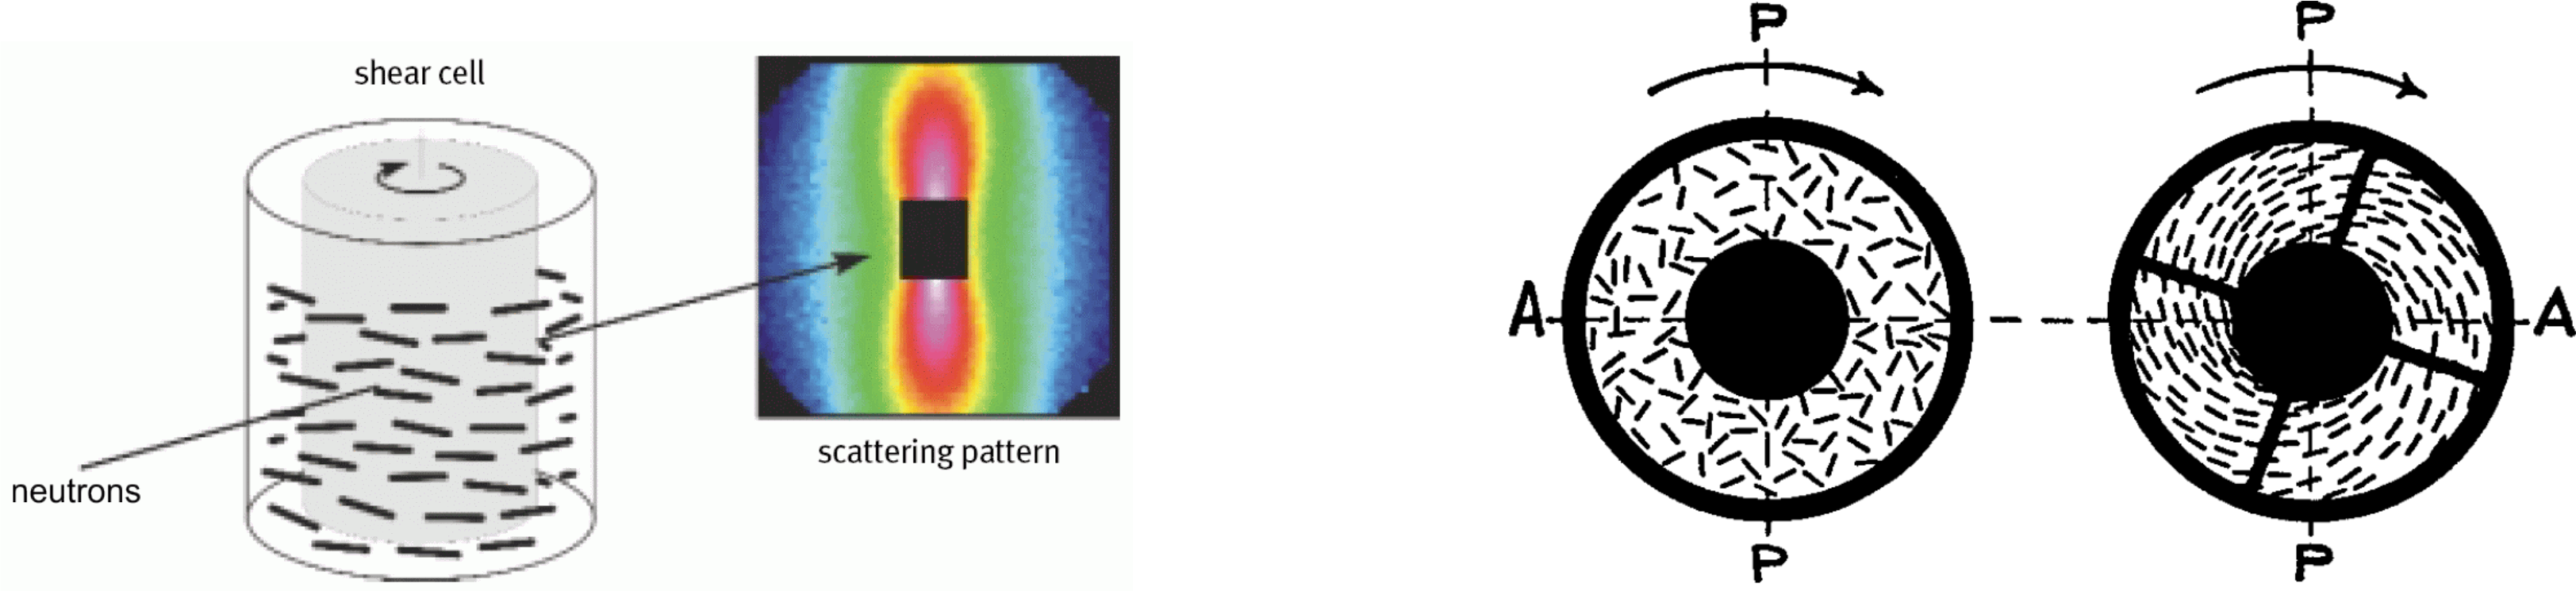
\includegraphics[width=\textwidth]{sheared_cylinders_n_phi0.png}
\end{center}
\caption{Shear orientation of micelles in a shear cell with the
corresponding SANS-pattern. The orientation of rods at rest and under shear according to \cite{Scheraga1951} are shown on th e right as a top view on the cuette cell.} \label{sheared_cylinders1}
\end{figure}

\begin{figure}[htb]
\begin{center}
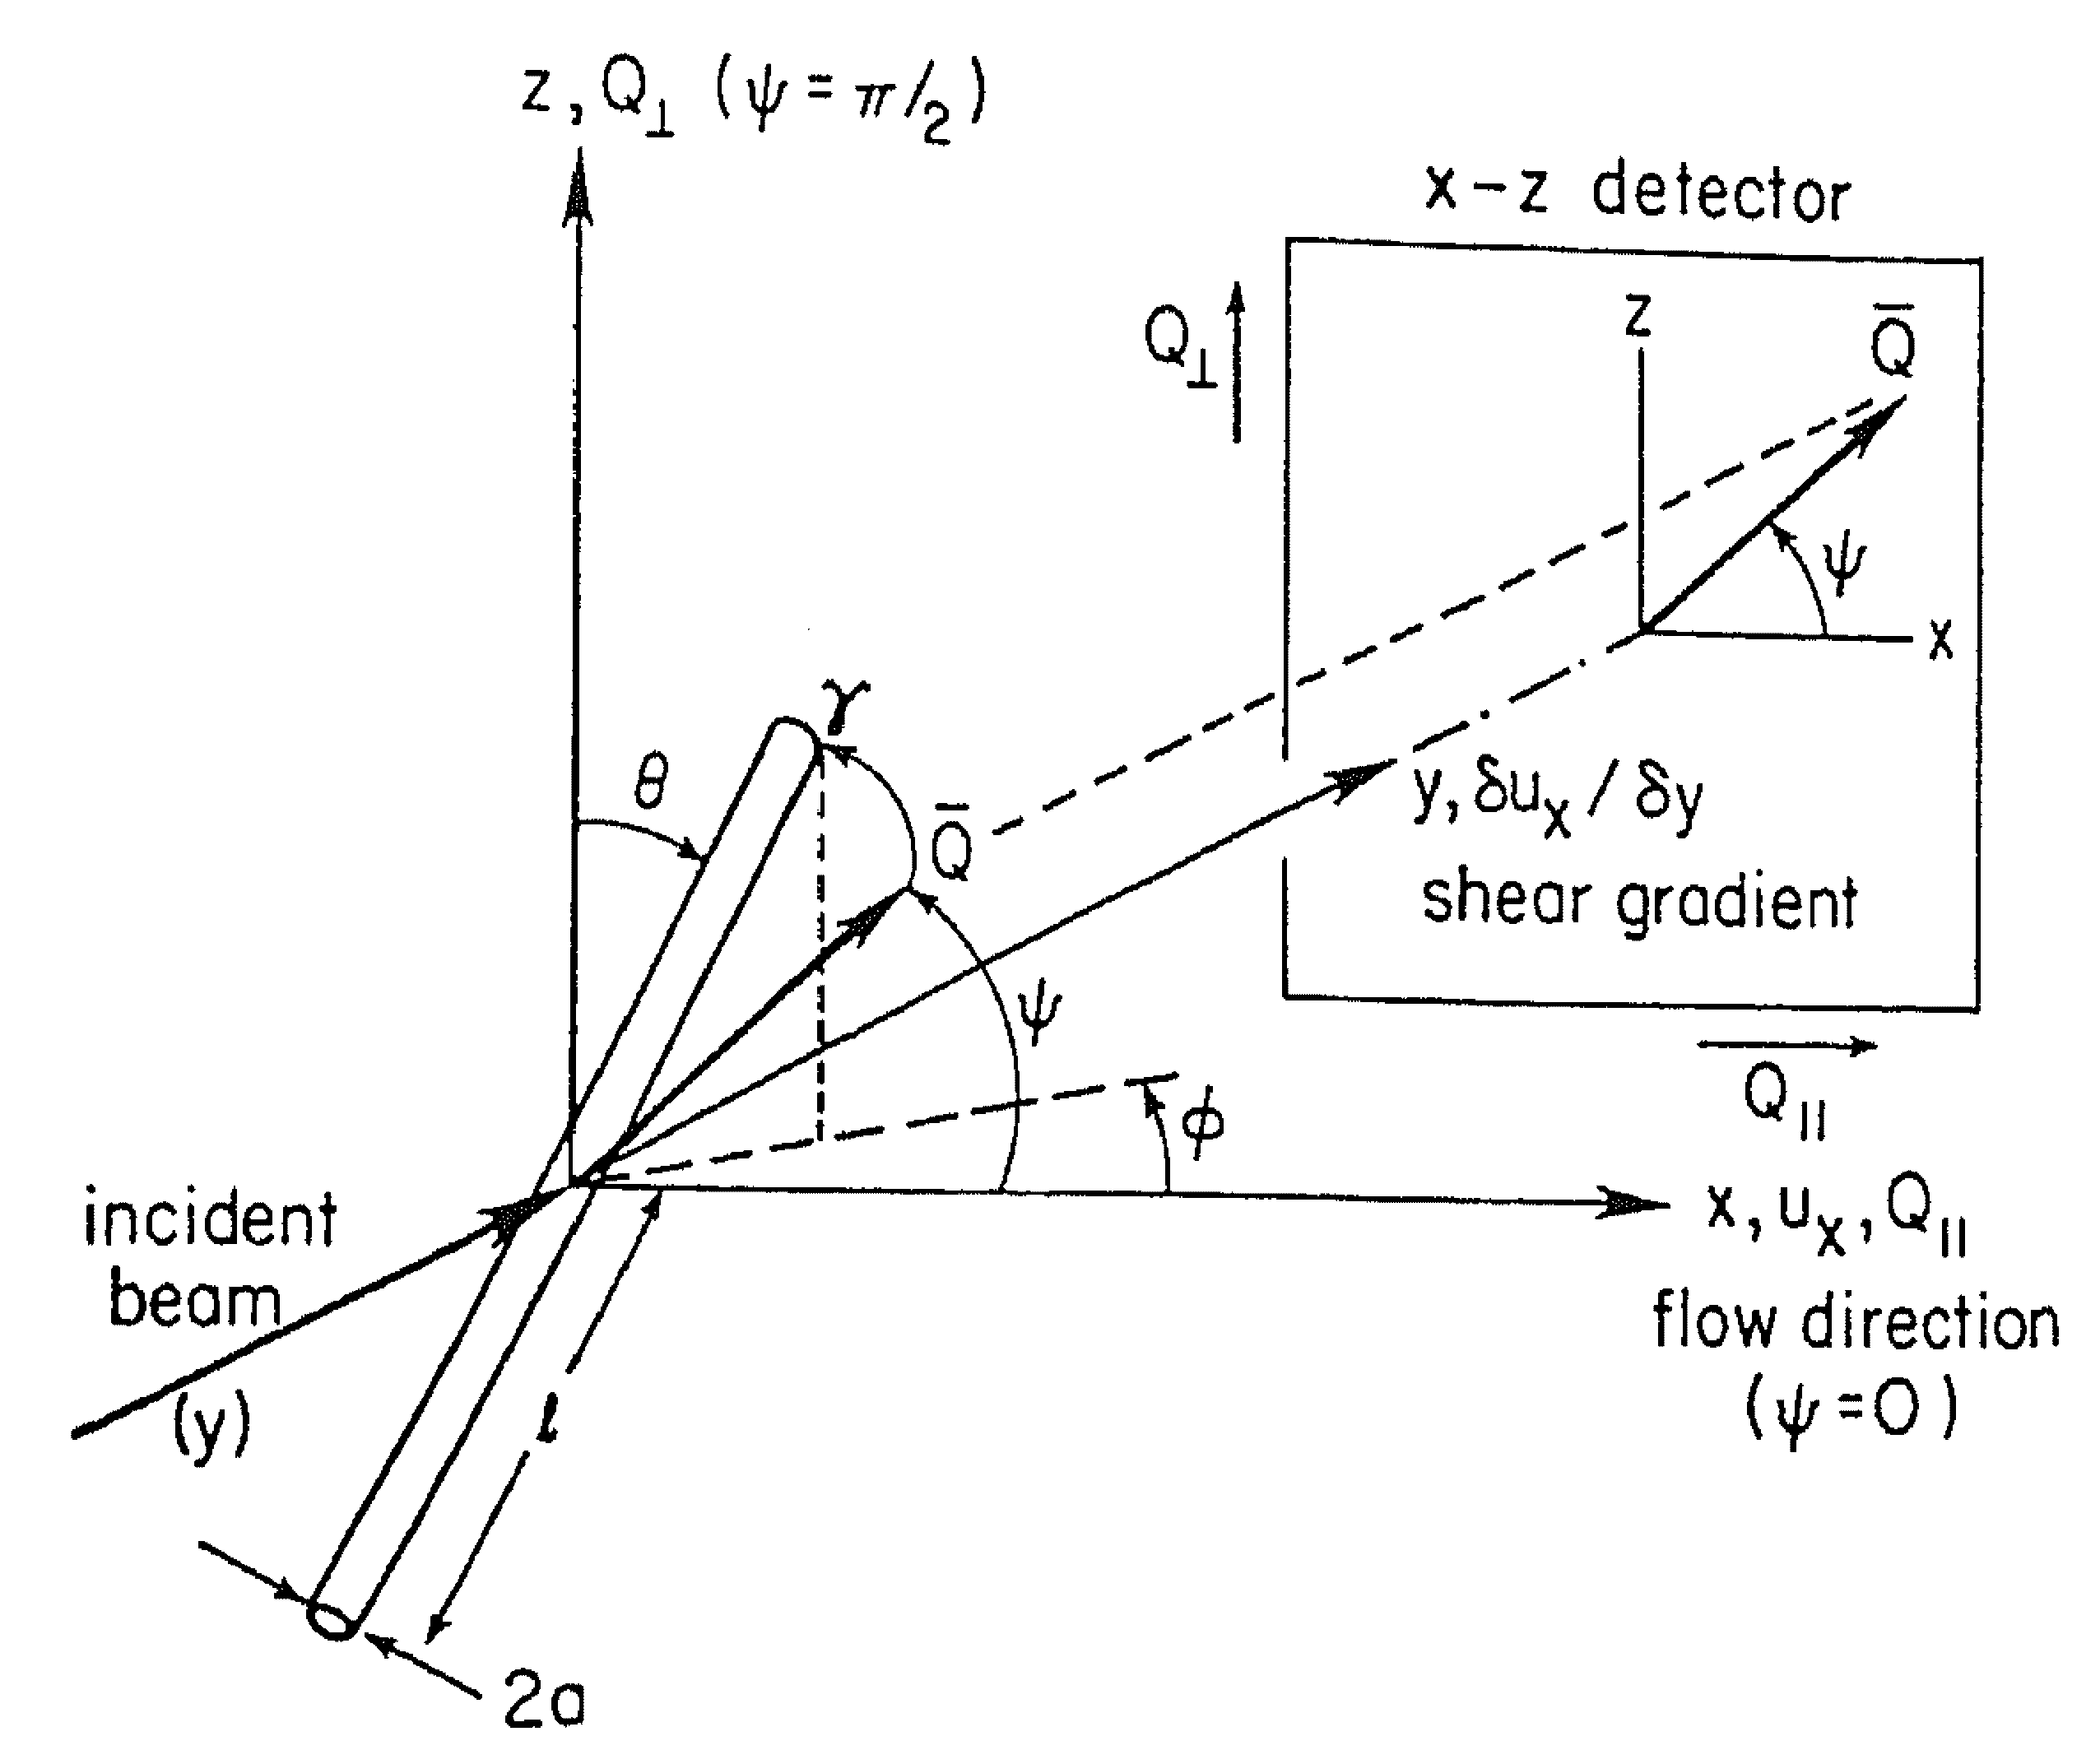
\includegraphics[width=0.7\textwidth]{shear_cuette_SANS_geometry.png}
\end{center}
\caption{Cartesian and angular coordinates referred to the center
of a cylindrical micelle at origin \cite{Hayter1984}. The relationship to the
spectrometer geometry is shown schematically. The momentum
transfer, $Q$, lies in the $z-x$ plane.}
\label{shear_cuette_SANS_geometry}
\end{figure}

The scattering from monodisperse dilute (non-interacting)
isotropic solution of anisotropic micelles is given by \cite{Hayter1984}
\BE
I(Q) =
\left< \vert K_\text{CylSh}(Q)\vert^2 \right>_Q \label{IQ_av}
\EE
where $K(Q)$
is the form factor for a micelle at a given orientation relative
to the momentum transfer $Q$ and $\left<\right>_Q$ denotes an
average over all such orientations.


For a cylindrical shell of length $L$, core diameter $2R$, and shell thickness $t$ the form
factor is given by:
\begin{align}
\begin{split}
K_\text{CylSh}\left(Q,\dots,\gamma\right)  = &
                  \hspace{\breites} K_\text{Cyl}\left(Q,\eta_\text{core}-\eta_\text{shell},R,L,\gamma\right) \\
                               & +  K_\text{Cyl}\left(Q,\eta_\text{shell}-\eta_\text{solv},R+\Delta R,L,\gamma\right)
\end{split}
\end{align}
with
\begin{align}
K_\text{Cyl}(Q,\Delta\eta,R,L,\gamma) & = 2 \pi R^2 L \Delta \eta
    \frac{J_1\left(Q R \sin\gamma\right)}{Q R \sin\gamma} \,
    \frac{\sin\left(\frac{QL}{2} \cos\gamma\right)}{\frac{QL}{2} \cos\gamma}
\end{align}
where $\gamma$ is the angle between $\mathbf{Q}$ and the cylinder
axis $\mathbf{n}$. $\eta_\text{core}$, $\eta_\text{shell}$, and $\eta_\text{solv}$ are the scattering length densities of the cylinder core, shell and solvent. $J_1(x)$ is the first order Bessel function of
the first kind. $\gamma$ can be calculated from the orientation
($\theta$, $\phi$) of the cylinder and the direction of the
scattering vector $\psi$ in the plane of the detector by
where $\gamma$ is the angle between $Q$ and the cylinder axis.

The scattering geometry for shear alignment is shown in Fig.
\ref{shear_cuette_SANS_geometry}. In general perfect alignment
will not be achieved, and an orientation distribution must be
employed such that the resultant scattering will be given by
\begin{align}
I(Q,\psi) &= \int_0^{2\pi} \int_0^\pi
p_\mathrm{HP}(\theta,\phi;\kappa)\, \left(K^2_\text{CylSh}(Q,\gamma^+)+K^2_\text{CylSh}(Q,\gamma^-)
\right) \sin\theta \mathrm{d}\theta \mathrm{d}\phi
\label{eq:IQShear_pHP}
\end{align}
with
\begin{align}
p_\mathrm{HP}(\theta,\phi;\kappa) & = \frac{(1-\cos
2\varPhi_0)(1+\sin^2\theta\cos 2\varPhi_0)^{3/2}}{4\pi\left[
1-\sin^2\theta\cos 2\varPhi_0\cos 2(\phi-\varPhi_0)\right]^2}
\end{align}
and
\BE
2\varPhi_0 = \arctan(8/\kappa)
\EE
$(\cos \varPhi_0,\sin \varPhi_0,0)^T$
is the direction of the most probable orientation $(\theta=\frac{\pi}{2};\phi=\varPhi_0)$. $\varPhi_0$ varies between $\varPhi_0=\frac{\pi}{4}$ for the isotropic case ($\kappa=0$)  to $\varPhi_0=0$ for perfect alignment ($\kappa\rightarrow \infty$).
\begin{figure}[htb]
\begin{center}
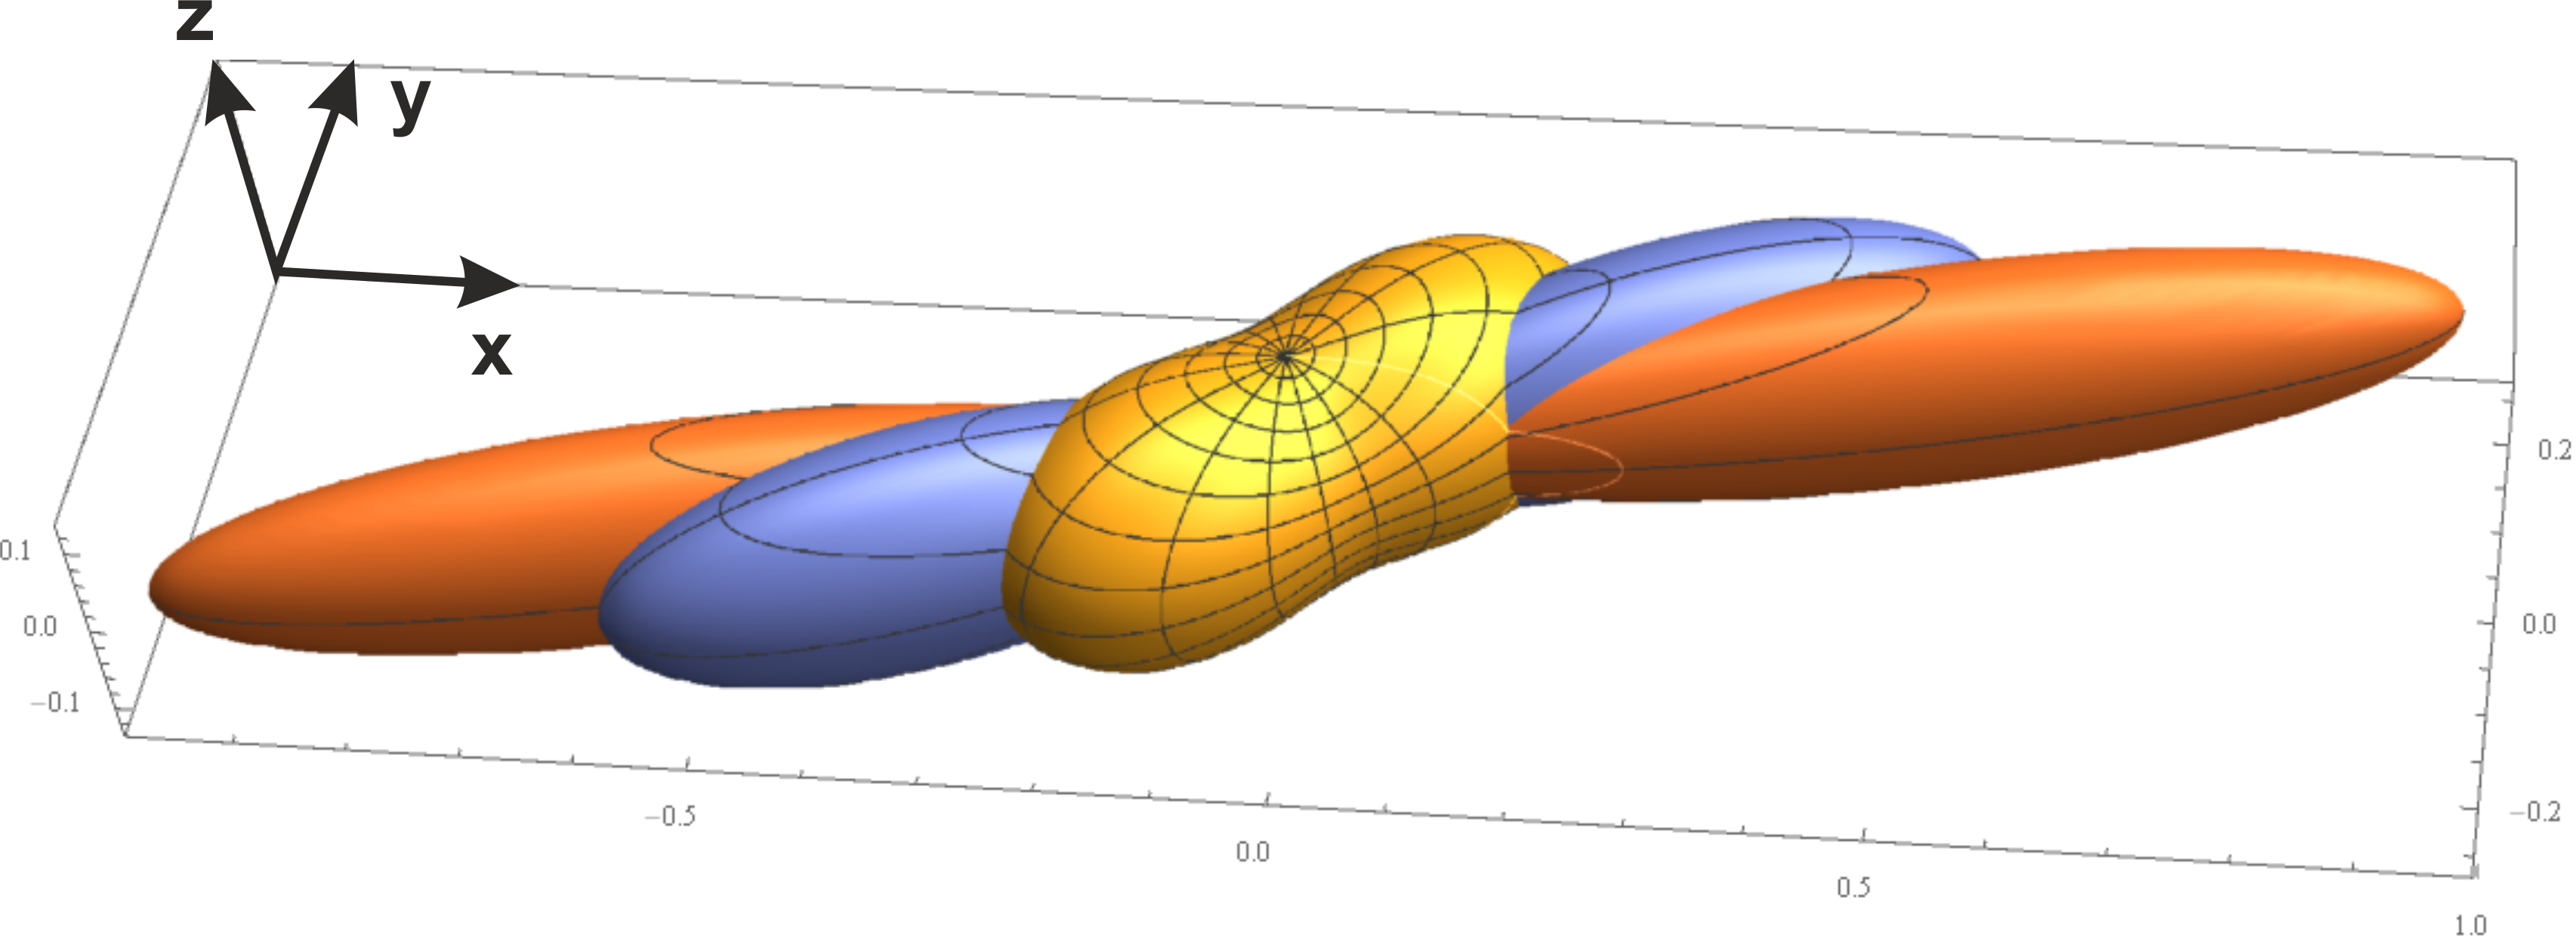
\includegraphics[width=\textwidth]{../images/form_factor/cylindrical_obj/pHP3D.png}
\end{center}
\caption{3D plot of the orientation distributions $2 p_\mathrm{HP}(\theta,\phi;\kappa={2})$ ({\bf \color[rgb]{1.0, 0.85, 0.0}yellow}), $p_\mathrm{HP}(\theta,\phi;\kappa{=}8)$ ({\bf\color[rgb]{0.36, 0.57, 0.9} blue}), $\frac12 p_\mathrm{HP}(\theta,\phi;\kappa{=}16)$ ({\bf\color[rgb]{1.0, 0.5, 0.0} orange}).} \label{fig:pHP3D}
\end{figure}
As the most probable direction is not the same as the flow direction, which is assumed to be the $x$-direction, and secondly that the beam is passing twice the cuette cell with flow direction $\mathbf{x}$ and $-\mathbf{x}$ we have to take the sum over two values for $\gamma^\pm$ in eq.\ \ref{eq:IQShear_pHP}. The angle $\gamma^\pm = \angle(\mathbf{Q,n}^\pm)$ between the scattering vector $\mathbf{Q}$ and the director of the cylinder axis $\mathbf{n}^\pm$ is
\begin{align}
\frac{\mathbf{Q}}{\abs{\mathbf{Q}}} &=
\begin{pmatrix}
\cos \psi \\
0  \\
\sin \psi
\end{pmatrix} \qquad
\frac{\mathbf{n}^\pm}{\abs{\mathbf{n}^\pm}} =
\begin{pmatrix}
\pm \sin \theta \cos \phi \\
\pm \sin \theta \sin \phi  \\
\cos \theta
\end{pmatrix} \\
\cos \angle(\mathbf{Q,n}^\pm) &= \cos \gamma^\pm = \frac{\mathbf{Q\cdot n}^\pm}{\abs{\mathbf{Q}}\abs{\mathbf{n}^\pm}} =  \pm \cos\psi \sin\theta \cos\phi + \sin\psi \cos\theta
\end{align}
For the reversed direction of the flow the $x$-component of the vector $\mathbf{n}^-$ changes its sign. In the original paper \cite{Hayter1984} one finds $\cos \gamma^-_\mathrm{HP} = \cos\psi \sin\theta \cos\phi - \sin\psi \cos\theta$, which, however, results to the same scattering intensity as the scattering intensity of a cylinder is invariant by a rotation of $\pi$, i.e. as $\cos(\pi+\gamma^-) =-\cos\gamma^- = \cos\gamma^-_\mathrm{HP}$ the resulting scattering patterns are the same for both value $\gamma^-$ and $\gamma^-_\mathrm{HP}$.

\vspace{5mm}

\uline{Input Parameters for model \texttt{Sheared Cylinders (HayterPenfold)}:}\\
\begin{description}
\item[\texttt{R}] radius of cylinders $R$
\item[\texttt{t}] shell thickness $t$
\item[\texttt{L}] cylinder length $L$
\item[\texttt{eta\_core}] scattering length density of cylinder core $\eta_\mathrm{core}$
\item[\texttt{eta\_shell}] scattering length density of cylinder shell $\eta_\mathrm{shell}$
\item[\texttt{eta\_solv}] scattering length density of solvent $\eta_\mathrm{solv}$
\item[\texttt{psi}] direction of scattering vector on the detector $\psi$
\item[{\texttt{sigma}}] width parameter of lognormal size distribution $\sigma$
\item[{\texttt{kappa}}] orientation distribution parameter $\kappa$
\end{description}

\uline{Note:}
\begin{itemize}
\item The size distribution is taken simultaneously over all parameters $R$, $t$ and $L$, so that their aspect rations stay always constant
\item The most probable orientation is not the $\mathbf{x}$-direction but tilted by the angle $\varPhi_0$. As in a rheometer with cuette geometry the beram is passing the sample twice the forward scattering is twice as large as in the model described in the next section.
\item As the orientation distribution is also not rotational symmetric around the direction of the most probably orientation and additional tilted against $\mathbf{x}$-axis the scattering pattern look less anisotropic than the other models in the following sections with the same order parameter $\kappa$.
\end{itemize}

%%%%%%%%%%%%%%%%%%%%%%%%%%%%%%%%%%%%%%%%%%%%%%%%%%%%%%%%%%%%%%%%%%%%%%%%%%%%%%%%%%
\newpage
\subsection{partly aligned anisotropic objects}
\label{sect:partlyalignedCylShell}
~\\

In contrast to the model of Hayter and Penfold \cite{Hayter1984} in section \ref{sect:ShearedCylinderHayterPenfold} here we use an orientation distribution with the most probably orientation along the $\mathrm{x}$-axis and independent on the polar angle $\phi$.
Therefore the coordination system is slightly differently defined in the Hayter-Penfold model of sheared cylinders.
\begin{figure}[htb]
\begin{center}
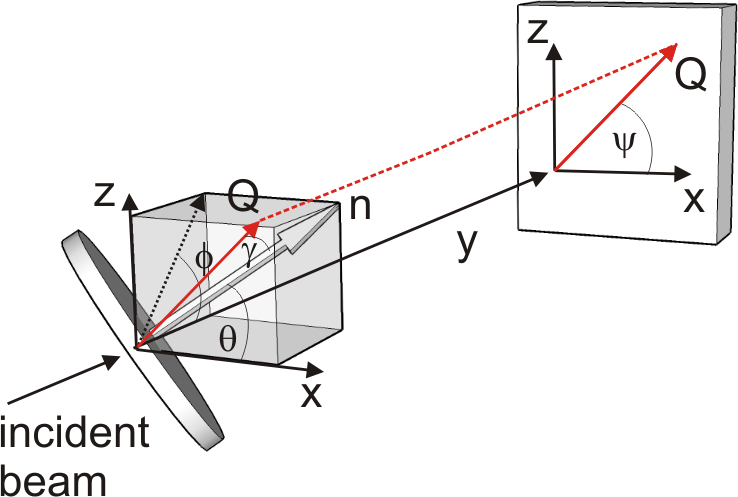
\includegraphics[width=0.7\textwidth]{../images/form_factor/cylindrical_obj/partly_aligned_discs.png}
\end{center}
\caption{Sketch of relative orientation $\mathbf{n}$ of partly
aligned cylinders or discs to the scattering vector $\mathbf{Q}$.}
\label{fig:partly_aligned_discs}
\end{figure}

\noindent The scattering amplitude of a cylindrical shell is given by
\begin{align}
\begin{split}
K_\text{CylShell}\left(Q,\dots,\gamma\right)  = &
\hspace{\breites} K_\text{Cyl}\left(Q,\eta_\text{core}-\eta_\text{shell},R,L,\gamma\right) \\
             & +  K_\text{Cyl}\left(Q,\eta_\text{shell}-\eta_\text{solv},R+\Delta R,L,\gamma\right)
\end{split}
\end{align}
with
\begin{align}
K_\text{Cyl}(Q,\Delta\eta,R,L,\gamma) & = 2 \pi R^2 L \Delta \eta
    \frac{J_1\left(Q R \sin\gamma\right)}{Q R \sin\gamma} \,
    \frac{\sin\left(\frac{QL}{2} \cos\gamma\right)}{\frac{QL}{2} \cos\gamma}
\end{align}
where $\gamma$ is the angle between $\mathbf{Q}$ and the cylinder
axis $\mathbf{n}$. $L$ is the length of the cylinder, $R$ its
radius, $\Delta\eta$ the scattering length density contrast relative
to the solvent and $J_1(x)$ is the first order Bessel function of
the first kind.

The scattering amplitude of an ellispoid of revolution is given by
\begin{align}
K_\text{Ell}(Q,\Delta\eta,R_\mathrm{e},R_\mathrm{p},\gamma) & = 4\pi R_\mathrm{e}^2 R_{p} \Delta\eta \frac{j_1(Qs)}{Qs}
\end{align}
with $s = \sqrt{R_\mathrm{p}\cos^2\gamma + R_\mathrm{e}\sin^2\gamma}$ and $j_1(x)$ being the spherical bessel function of first kind. $R_\mathrm{e}$ and $R_{p}$ are the equatorial and polar semi-axes of the spheroid, respectively.
The scattering amplitude of an ellipsoidal shell is given by
\begin{align}
\begin{split}
K_\text{EllShell}\left(Q,\dots,\gamma\right)  = &
\hspace{\breites} K_\text{Ell}\left(Q,\eta_\text{core}-\eta_\text{shell},R_{\mathrm{p}},R_{\mathrm{e}},\gamma\right) \\
             & +  K_\text{Ell}\left(Q,\eta_\text{shell}-\eta_\text{solv},R_{\mathrm{p}}+\Delta R,R_{\mathrm{e}}+\Delta R,\gamma\right)
\end{split}
\end{align}
$\gamma$ can be calculated from the orientation
($\theta$, $\phi$) of the cylinder and the direction of the
scattering vector $\psi$ in the plane of the detector by
\begin{align}
\frac{\mathbf{Q}}{\abs{\mathbf{Q}}} &=
\begin{pmatrix}
\cos \psi \\
0  \\
\sin \psi
\end{pmatrix} \qquad
\frac{\mathbf{n}}{\abs{\mathbf{n}}} =
\begin{pmatrix}
\cos \theta \\
\sin \theta \cos \phi  \\
\sin \theta \sin \phi
\end{pmatrix} \\
\cos \measuredangle(\mathbf{Q,n}) &= \cos \gamma = \frac{\mathbf{Q\cdot
n}}{\abs{\mathbf{Q}}\abs{\mathbf{n}}} = \cos\psi \cos\theta +
\sin\psi \sin\theta \sin\phi
\end{align}
If the orientation distribution of the orientation vector $\mathbf{n}$ is described by $p(\theta,\phi,\kappa)$
so that the scattering intensity is given by
\begin{align}
I_\mathrm{p.a.CylShell}(Q) & =
            \int_0^\pi d\theta \int_0^{2\pi} d\phi \, \,
                K^2_\text{CylShell}\left(Q,\dots,\gamma\right)\,p(\theta,\phi;\kappa)\,\sin(\theta) \label{eq:HPshearCyl}\\
I_\mathrm{p.a.EllShell}(Q) & =
            \int_0^\pi d\theta \int_0^{2\pi} d\phi \, \,
                K^2_\text{EllShell}\left(Q,\dots,\gamma\right)\,p(\theta,\phi;\kappa)\,\sin(\theta)  \label{eq:HPshearEll}
\end{align}
For this form factor it is assumed that the orientation distribution is independent of $\phi$,
i.e. $p(\theta,\phi;\kappa)=p(\theta;\kappa)$ and that $p(\theta;\kappa)=p(\pi-\theta;\kappa)$, which means that turning the cylinder by 180$^\circ$ results in the same scattering intensity.
Several orientation distributions have been implemented in a way that their resulting order parameter $S_2$ can have values between -0.5 and 1, which correspond to perfect alignment perpendicular to the $\mathrm{x}$ axis and perfect alignment parallel to it. All probability distributions have been normalized
\begin{align}
\int_0^\pi \int_0^{2\pi} p(\theta,\phi;\kappa) \sin \theta \, d\theta \, d\phi&=1
\end{align}
\begin{figure}[htb]
\begin{center}
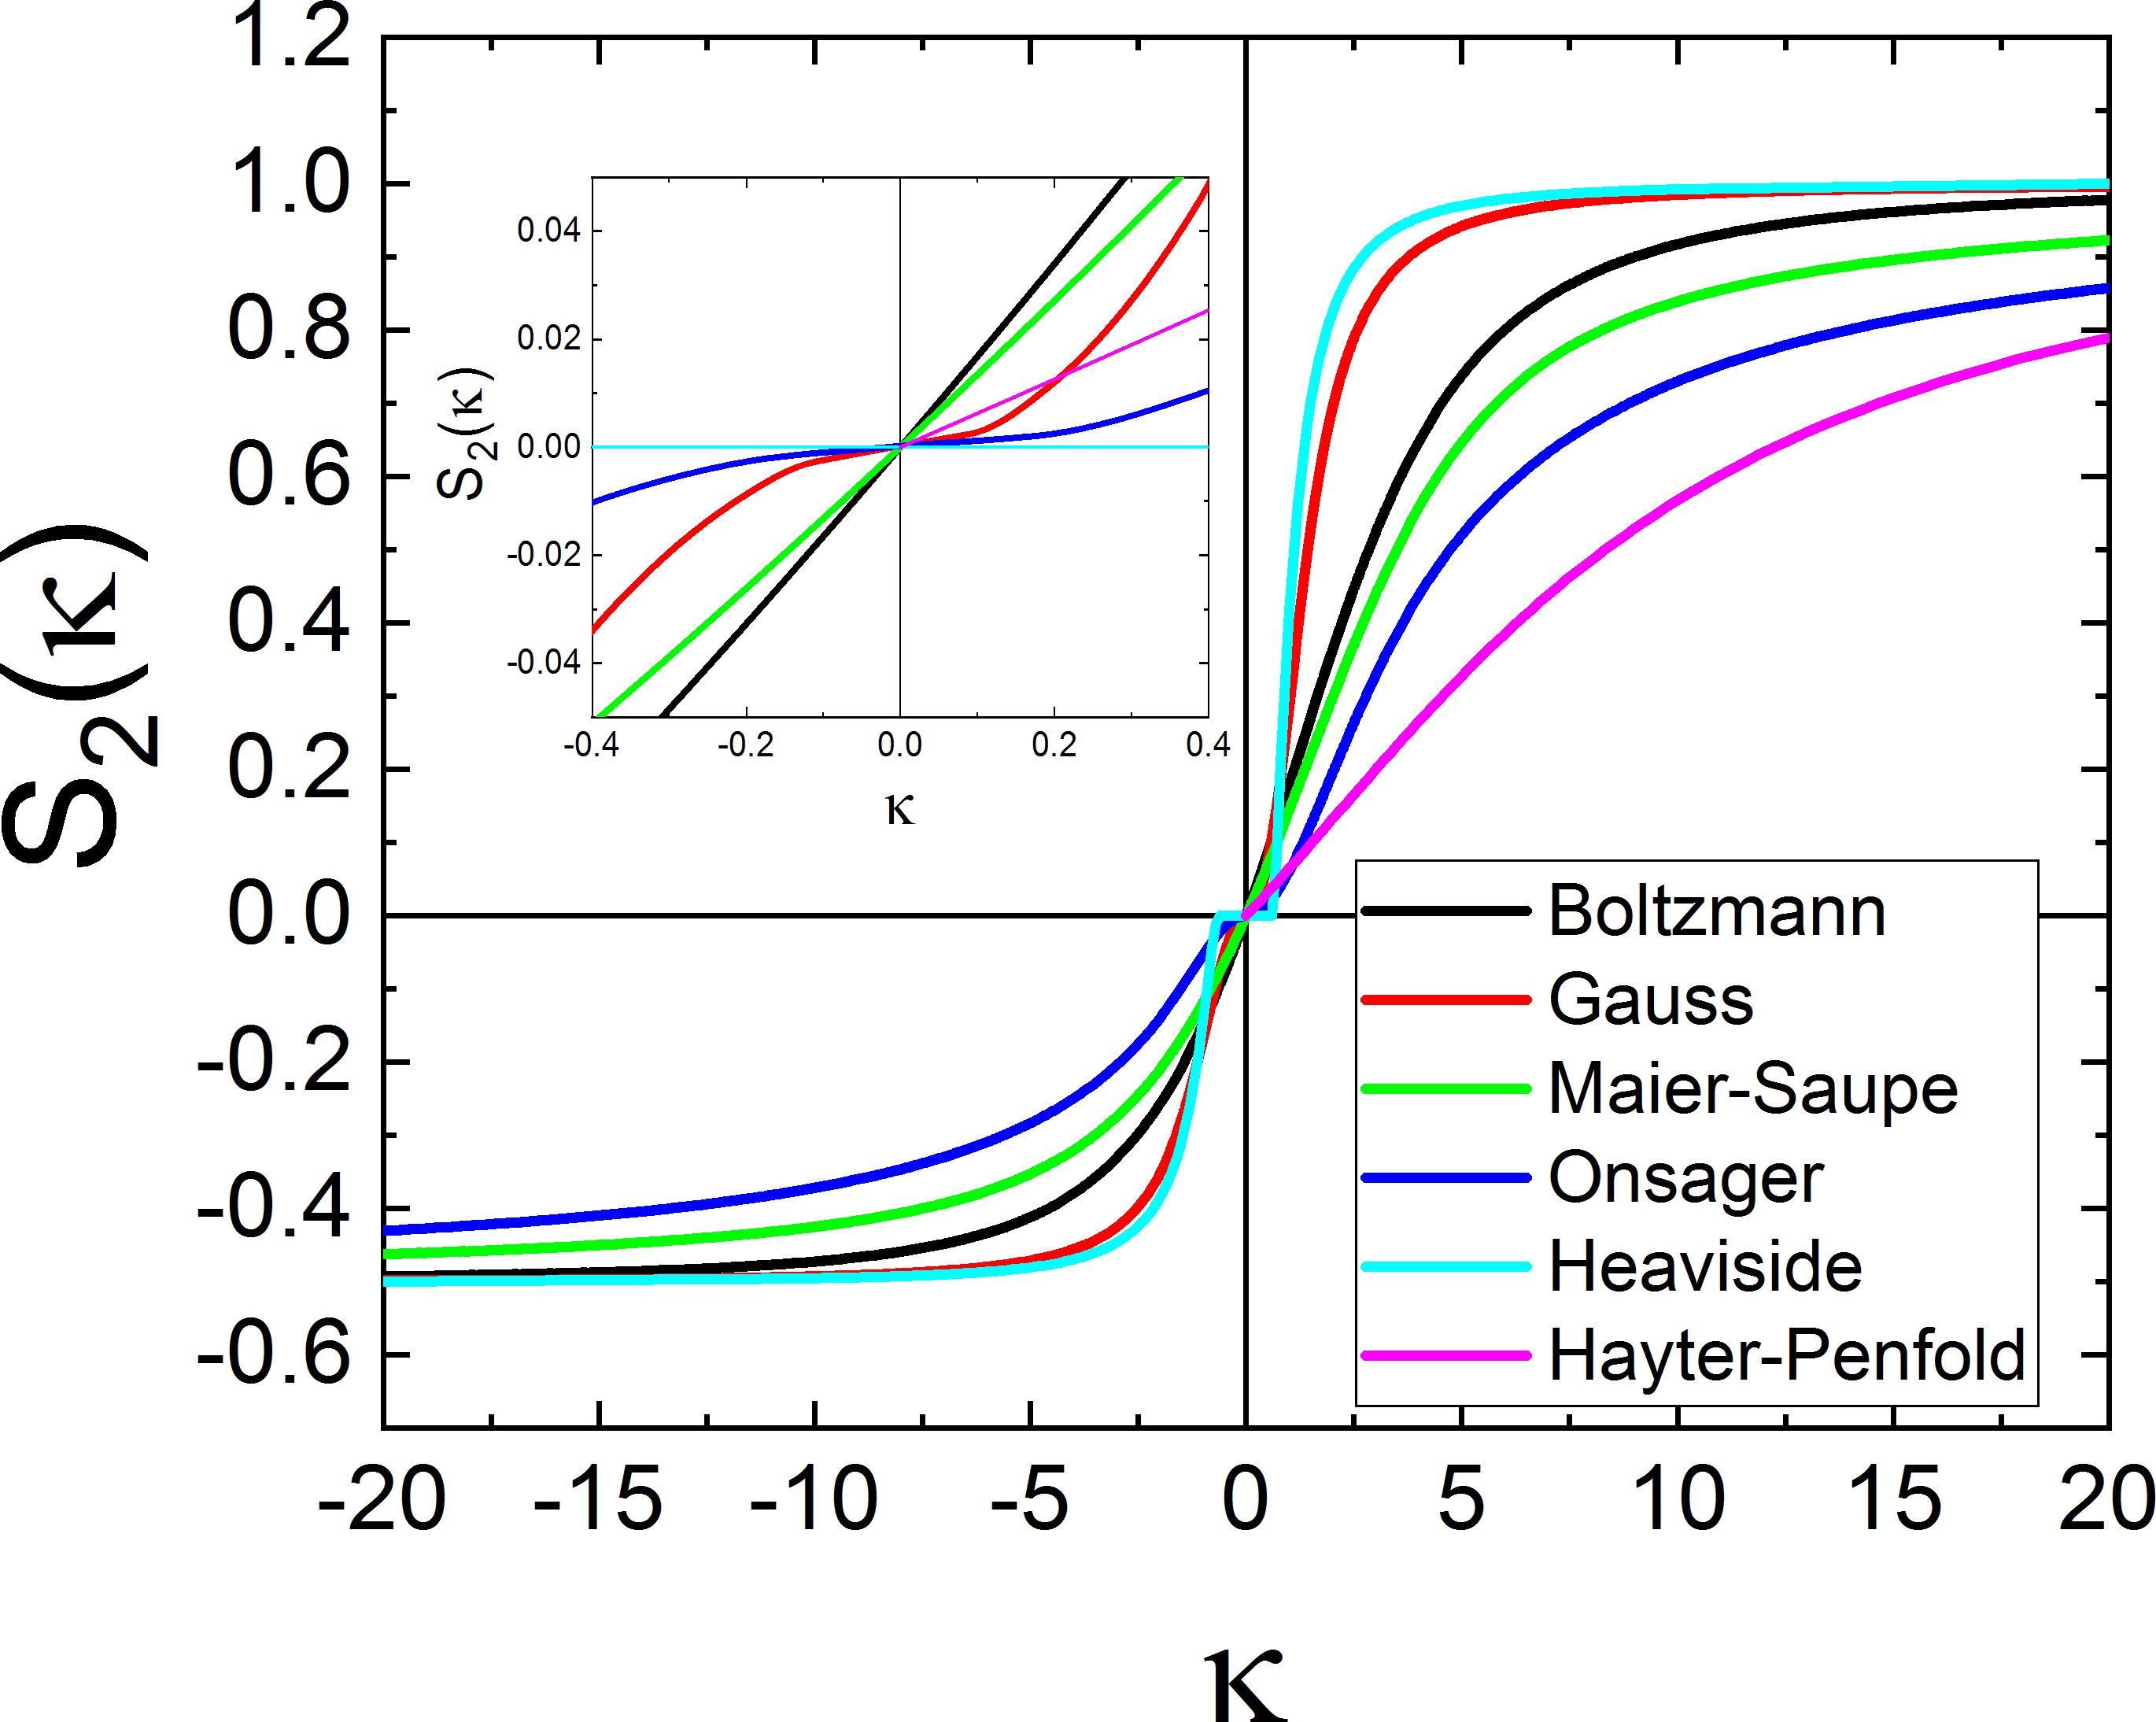
\includegraphics[width=0.75\textwidth]{../images/form_factor/cylindrical_obj/S2(kappa).png}
\end{center}
\caption{Order parameter $S_2(\kappa)$ for the orientation distributions described in the next subsections.}
\label{fig:S2_kappa}
\end{figure}

\begin{table}[htb]
\centering
\caption{Values for $\kappa$ to obtain certain order parameters $S_2(\kappa)$ for the different orientation distributions $p(\theta,\phi,\kappa)$.}
\label{tab:kappas}
\begin{tabular}{|l|llllllllll|}
\toprule
\diagbox{$p(\theta,\phi,\kappa)$}{$S_2(\kappa)$}  & -0.45    & -0.4    & -0.2    & 0 & 0.2    & 0.4    & 0.6    & 0.8    & 0.9    & 0.95    \\ \midrule
Gauss       & -3.739 & -1.62  & -1.128 & 0 & 0.83  & 1.220 & 1.686 & 2.576 & 3.762 & 5.4    \\
Boltzmann   & -7.141 & -4.59  & -1.431 & 0 & 1.114 & 2.218 & 3.581 & 5.989 & 9     & 13.08 \\
Maier-Saupe & -15    & -7.49  & -1.874 & 0 & 1.367 & 2.709 & 4.444 & 8.241 & 15.59 & 30.54 \\
Onsager     & -28.43 & -13.35 & -2.918 & 0 & 2.042 & 3.629 & 6.313 & 13.92 & 28.96 & 58.99 \\
Heavyside   & -3.108 & -2.157 &	-1.129 & 0 & 0.794 & 0.982 & 1.267 & 1.868 & 2.692 & 3.840 \\
Hayter-Penfold   & $\varnothing$ & $\varnothing$&	$\varnothing$ & 0 & 3.008 & 6.269 & 10.93 & 20.8 & 34.91 & 55.64  \\ \bottomrule
\end{tabular}
\end{table}

The order parameters $S_2$ can be calculated by
\begin{align}
S_2(\kappa) &=
\int_0^\pi \int_0^{2\pi}
                p(\theta,\phi;\kappa) \frac12 \left(3\cos^2\theta - 1\right) \sin \theta \, \mathrm{d}\theta\, \mathrm{d}\phi \nonumber \\
&= \int_0^\pi 2\pi
                p(\theta;\kappa) \frac12 \left(3\cos^2\theta - 1\right) \sin \theta \, \mathrm{d}\theta
\label{eq:S2kappa}
\end{align}
\begin{figure}[htb]
\captionsetup[subfigure]{position=b}
\centering
\subcaptionbox{Onsager orientation distribution for $\kappa=3$.  \label{fig:pOnsager3D1} }{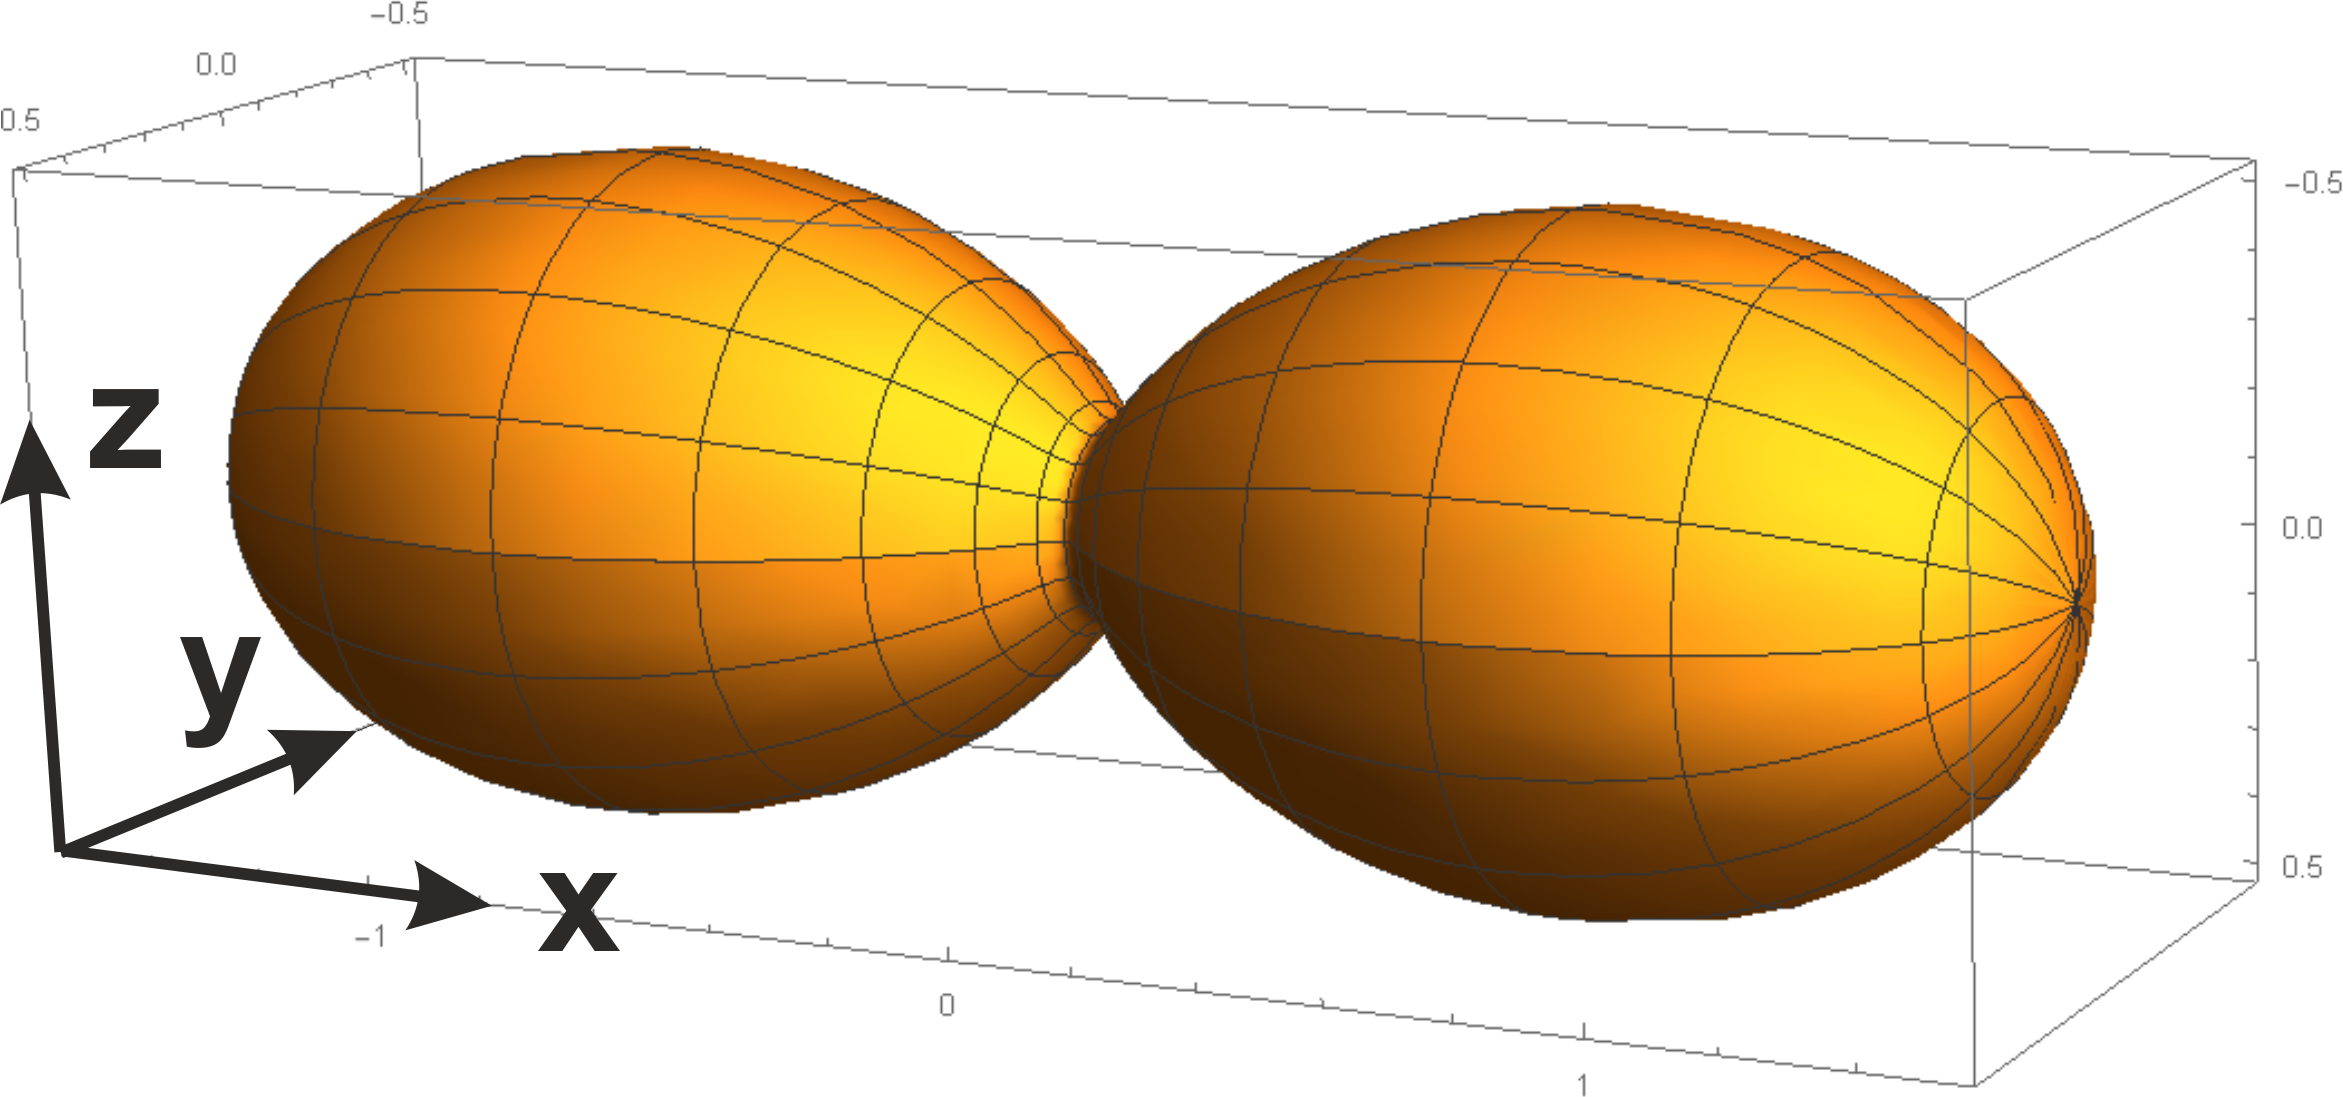
\includegraphics[width=0.55\textwidth]{../images/form_factor/cylindrical_obj/pOnsager(3).png}}
\hfill
\subcaptionbox{Onsager orientation distribution for $\kappa=-3$. \label{fig:pOnsager3D2}}{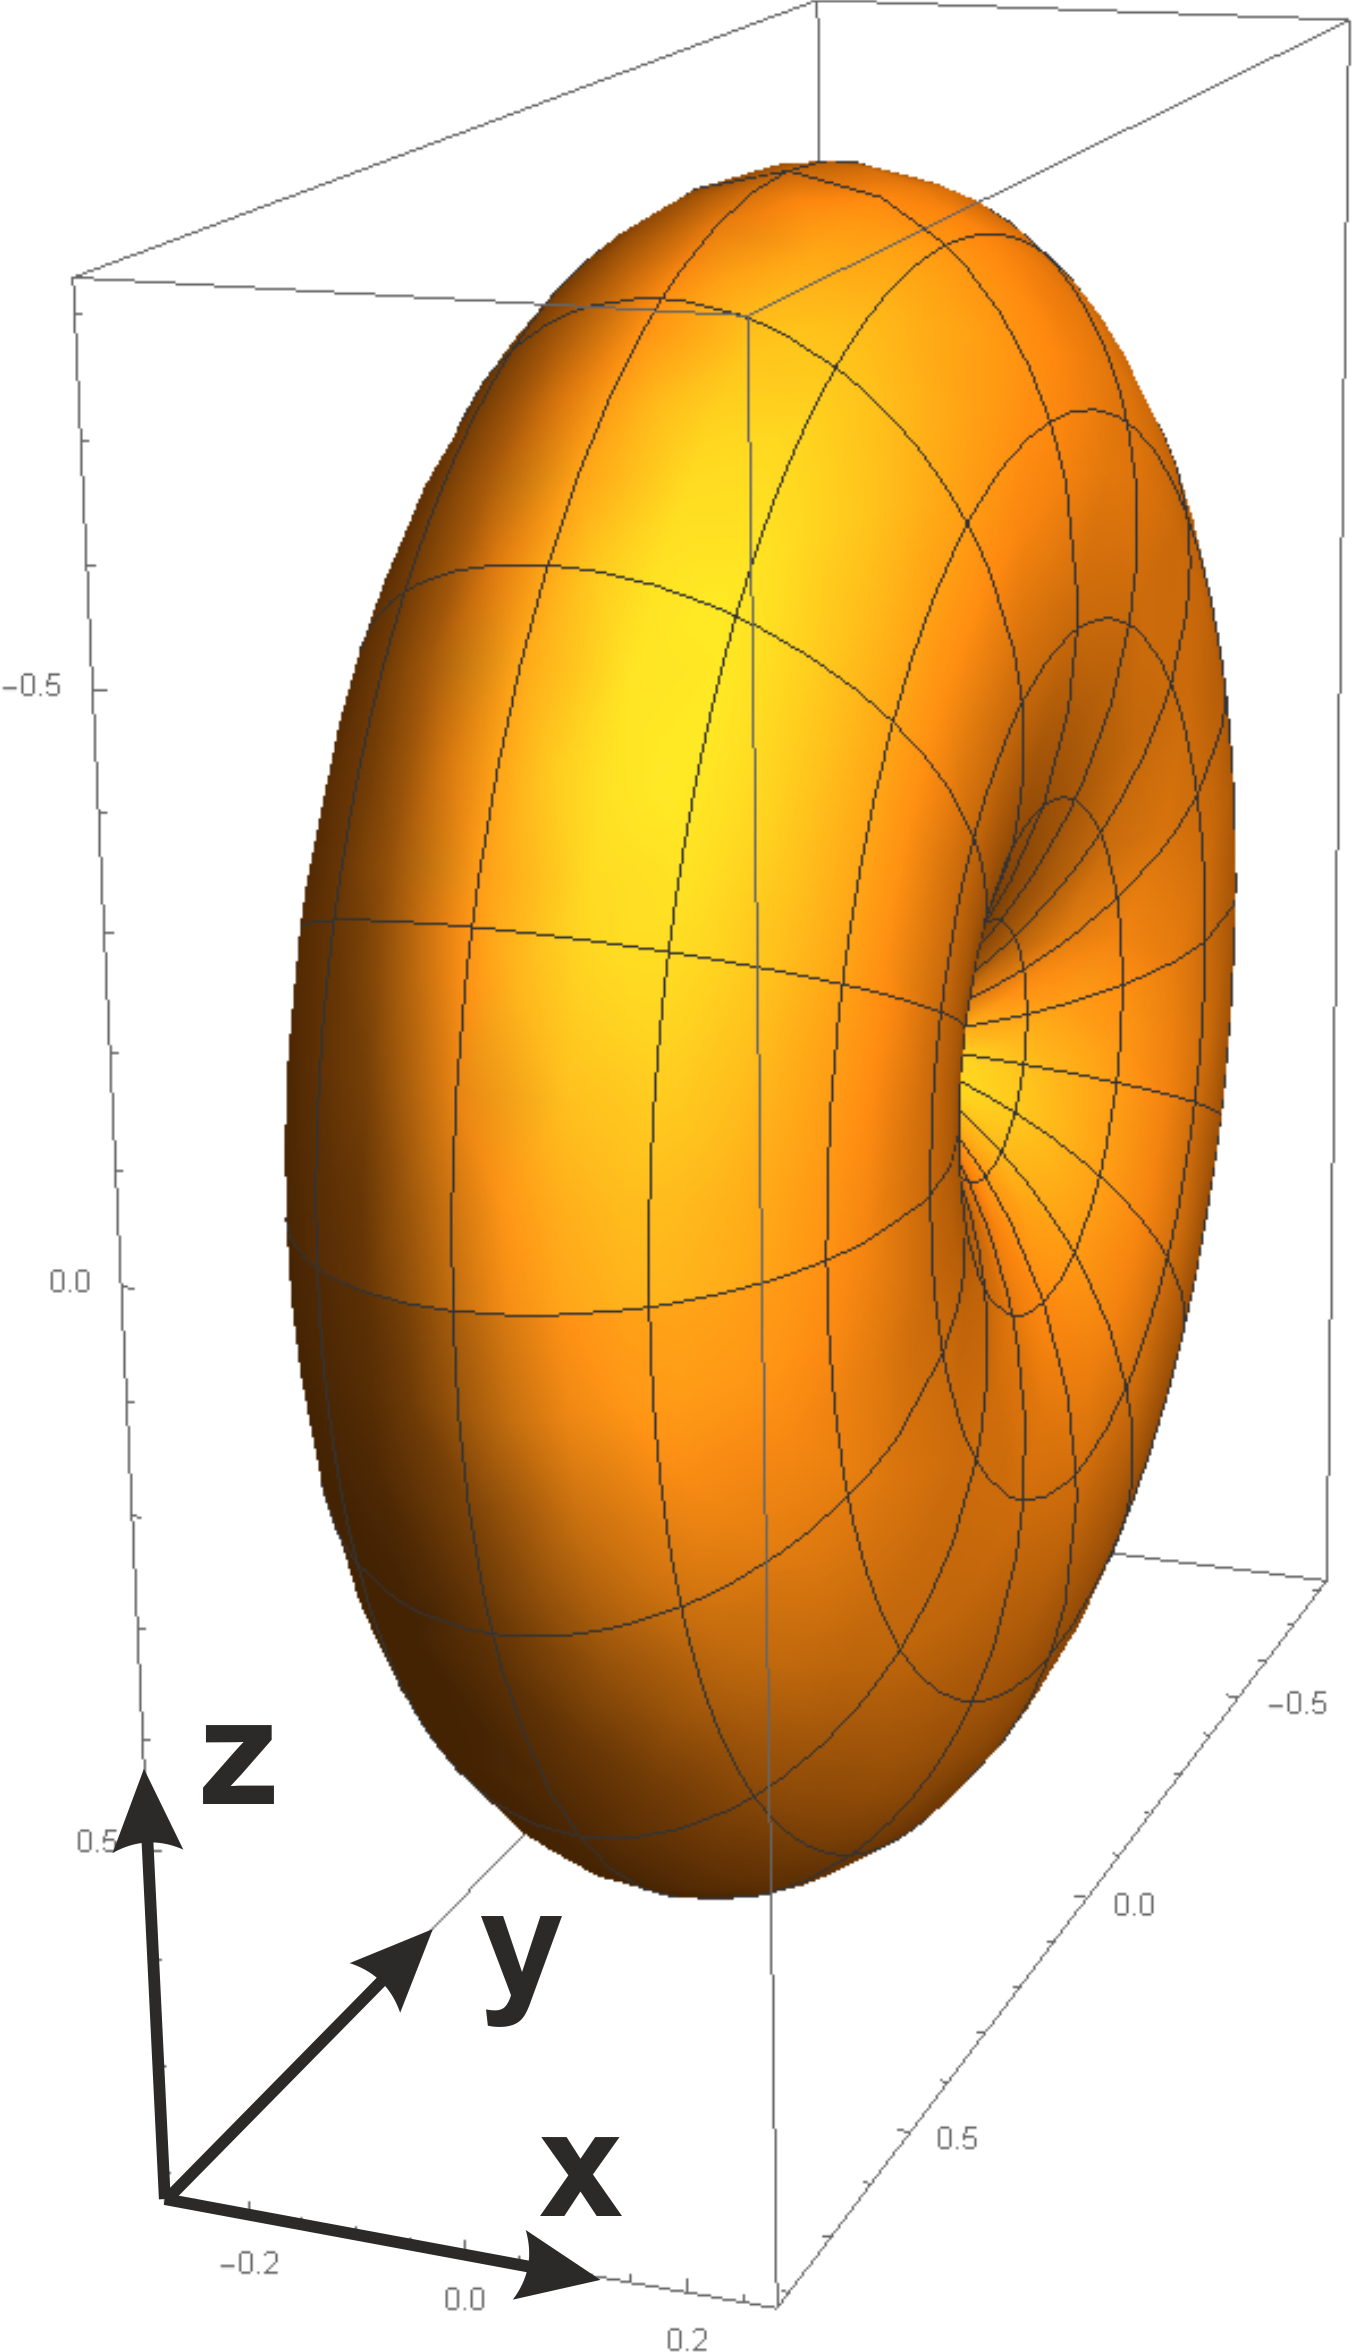
\includegraphics[width=0.4\textwidth]{../images/form_factor/cylindrical_obj/pOnsager(-3).png}}
\caption{Orientation distributions are are all independent on $\phi$ and have for $\kappa>0$ a positive order parameter, i.e. the most probable orientation is in the $\mathbf{x}$-direction and for $\kappa<0$ a negative order parameter, i.e. the most probable orientation lies in the $\mathbf{zy}$-plane}
\label{fig:pOnsager3D}
\end{figure}

\begin{figure}[htb]
\begin{center}
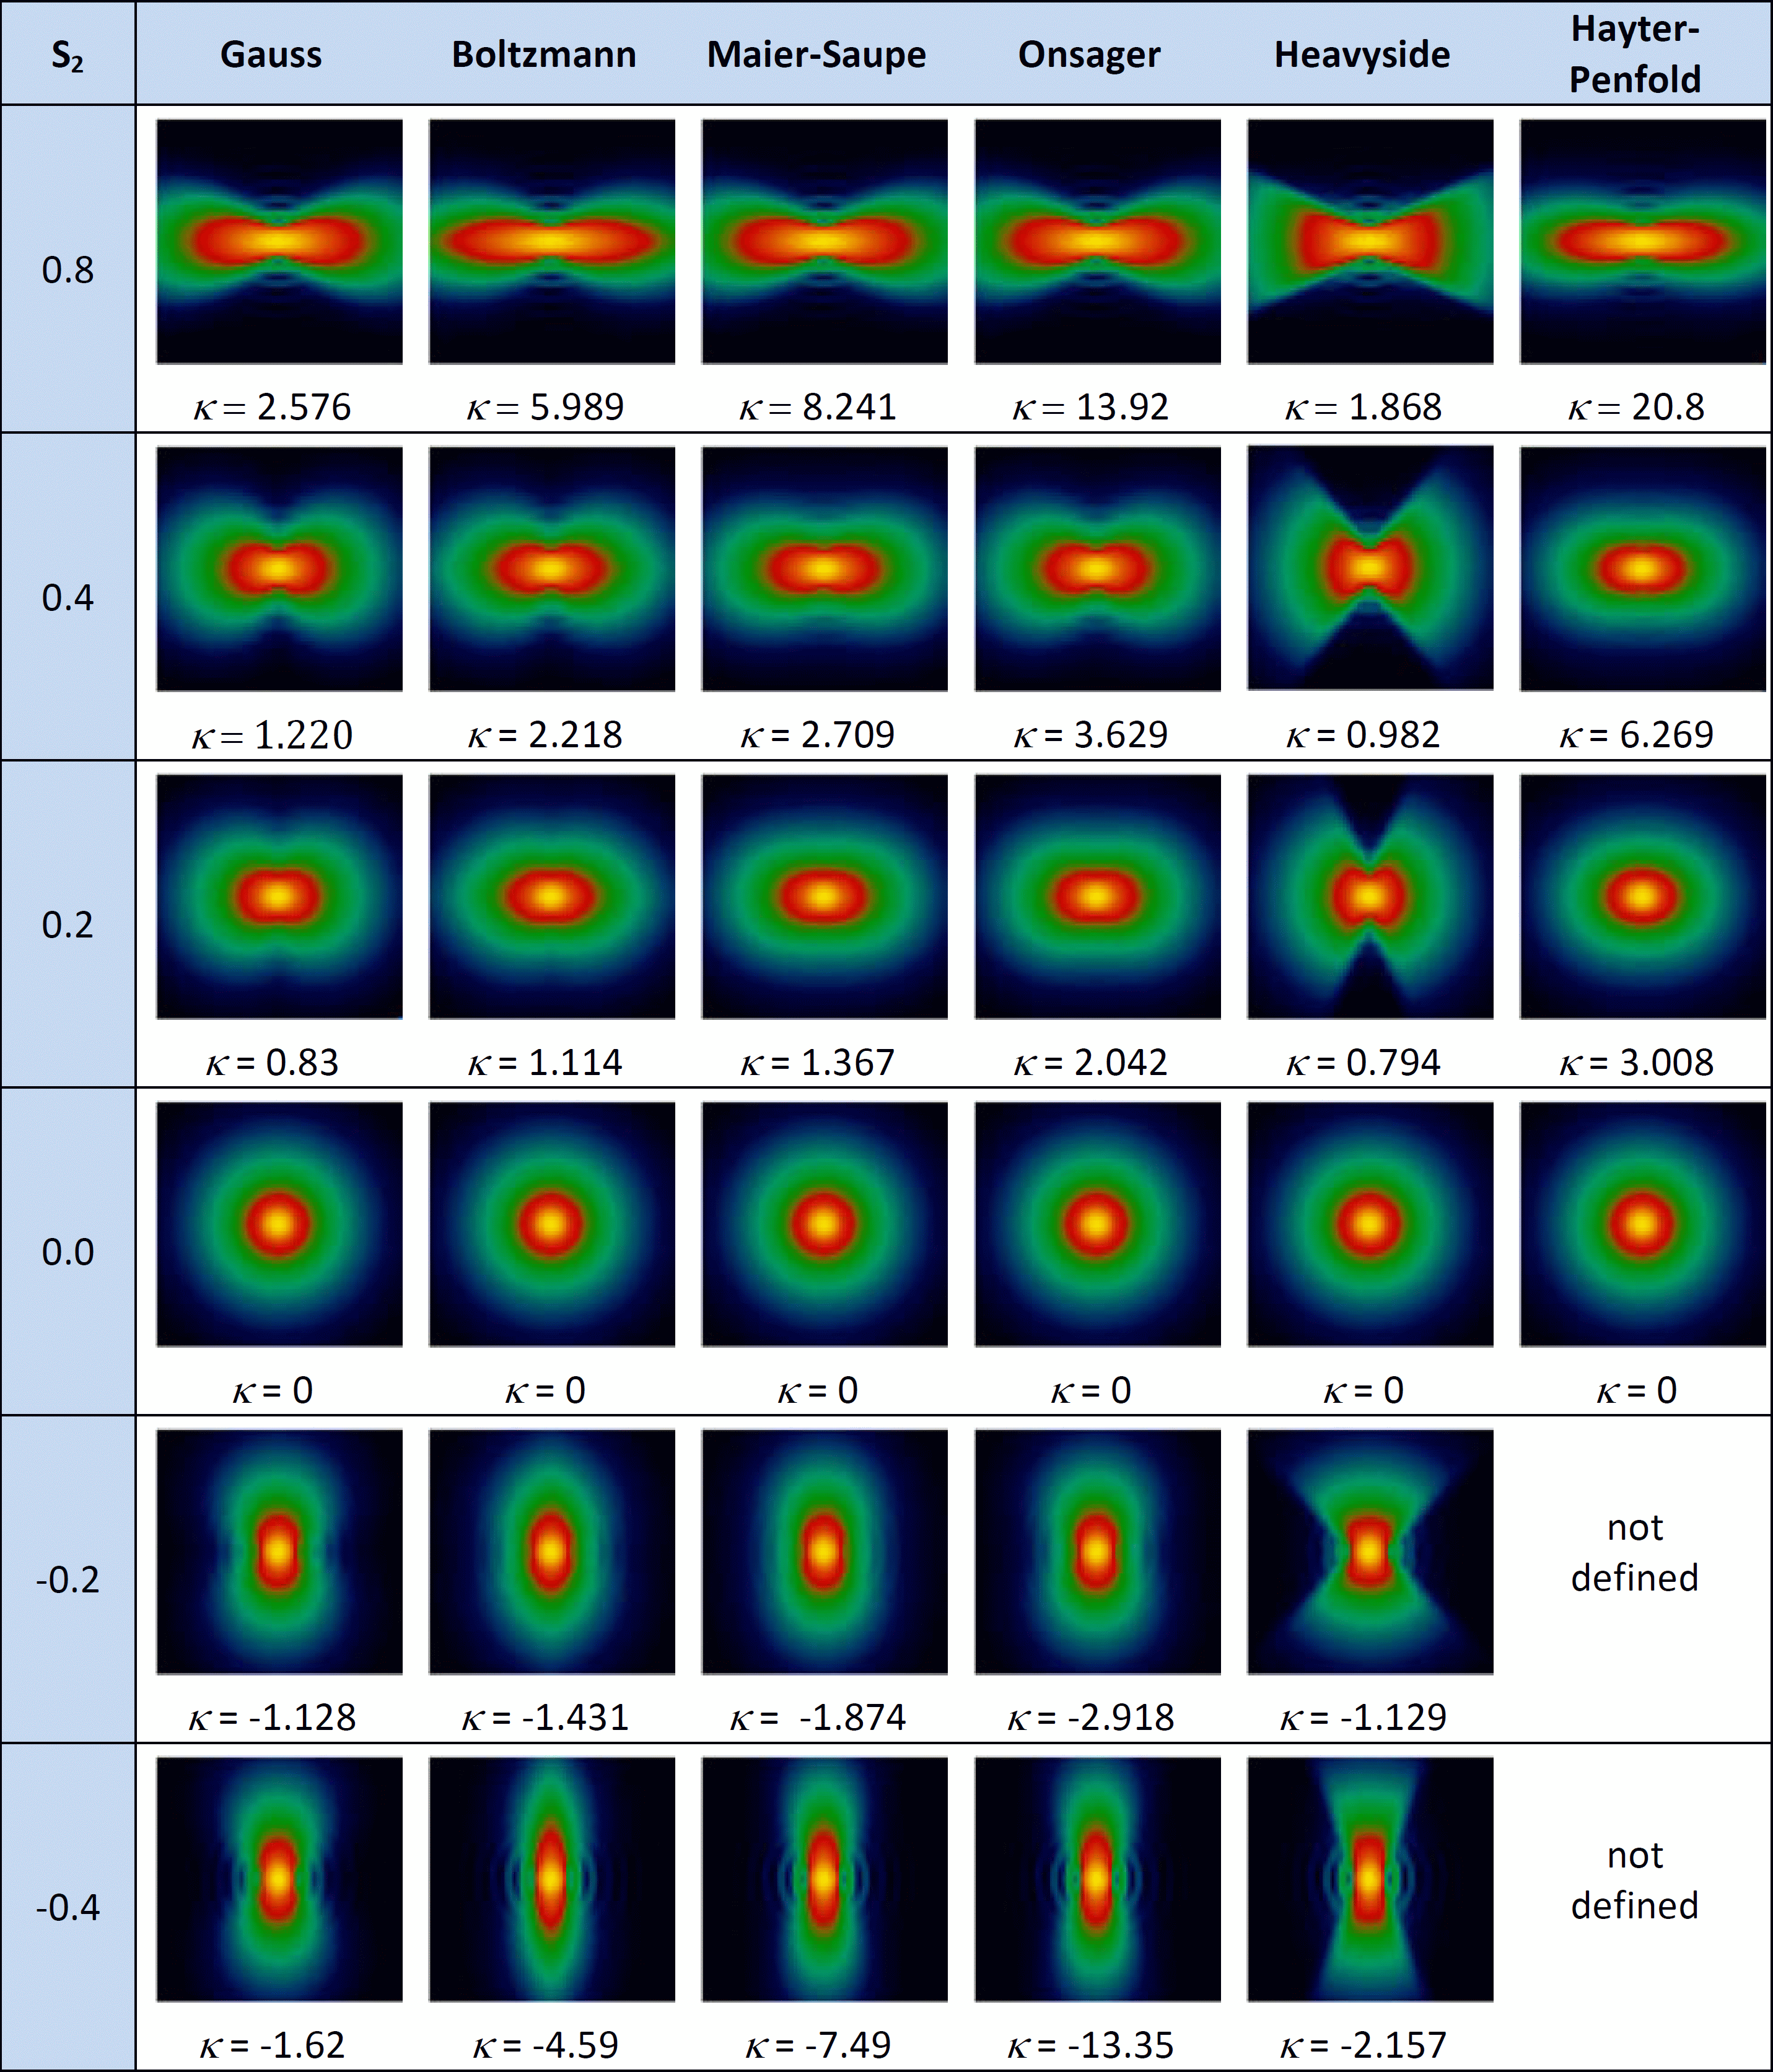
\includegraphics[width=0.95\textwidth]{../images/form_factor/cylindrical_obj/pXXXcomparison.png}
\end{center}
\caption{comparison of different orientation distributions with the same order parameter.}
\label{fig:S2_comparision}
\end{figure}

The order parameter for the Hayter-Penfold orientation distribution has been calculated by performing first a coordination transformation of the polar coordinates with $\mathbf{z}$ being the polar axis to coordination system with a polar axis pointing into the direction of the most probable orientation. The order parameter $S_2(\kappa)$ in eq.\ \ref{eq:S2kappa} is then calculated in this new polar coordinate system.

The form factors additional contain already a size distribution to profit from the speed enhancement by using a specialized multidimensional integration routine. The size distribution is included as
\begin{align}
I(Q) &= \int_0^\infty \mathrm{LogNorm}(\nu,\sigma,1) I_\mathrm{p.a.CylShell}(Q,R\nu,\Delta R\nu,L\nu) \, \mathrm{d}\nu \\
\end{align}
and
\begin{align}
I(Q) &= \int_0^\infty \mathrm{LogNorm}(\nu,\sigma,1) I_\mathrm{p.a.EllShell}(Q,R_\mathrm{p}\nu,\Delta R\nu,R_\mathrm{e}\nu) \, \mathrm{d}\nu
\end{align}
 with
\begin{align}
\mathrm{LogNorm}(\nu,\sigma,\mu) &= \frac{1}{\sqrt{2\pi}\sigma}\frac{1}{\nu} \exp\left(-\frac{(\ln(\nu/\mu))^2}{2\sigma^2}\right)
\end{align}

%%%%%%%%%%%%%%%%%%%%%%%%%%%%%%%%%%%%%%%%%%%%%%%%%%%%%%%%%%%%%%%%%%%%%%%%%%%%%%%%%%%%%%%%%%%%%%%%%%%%%%%%%
\clearpage
\subsubsection{Maier-Saupe orientation distribution} ~\\

\begin{figure}[htb]
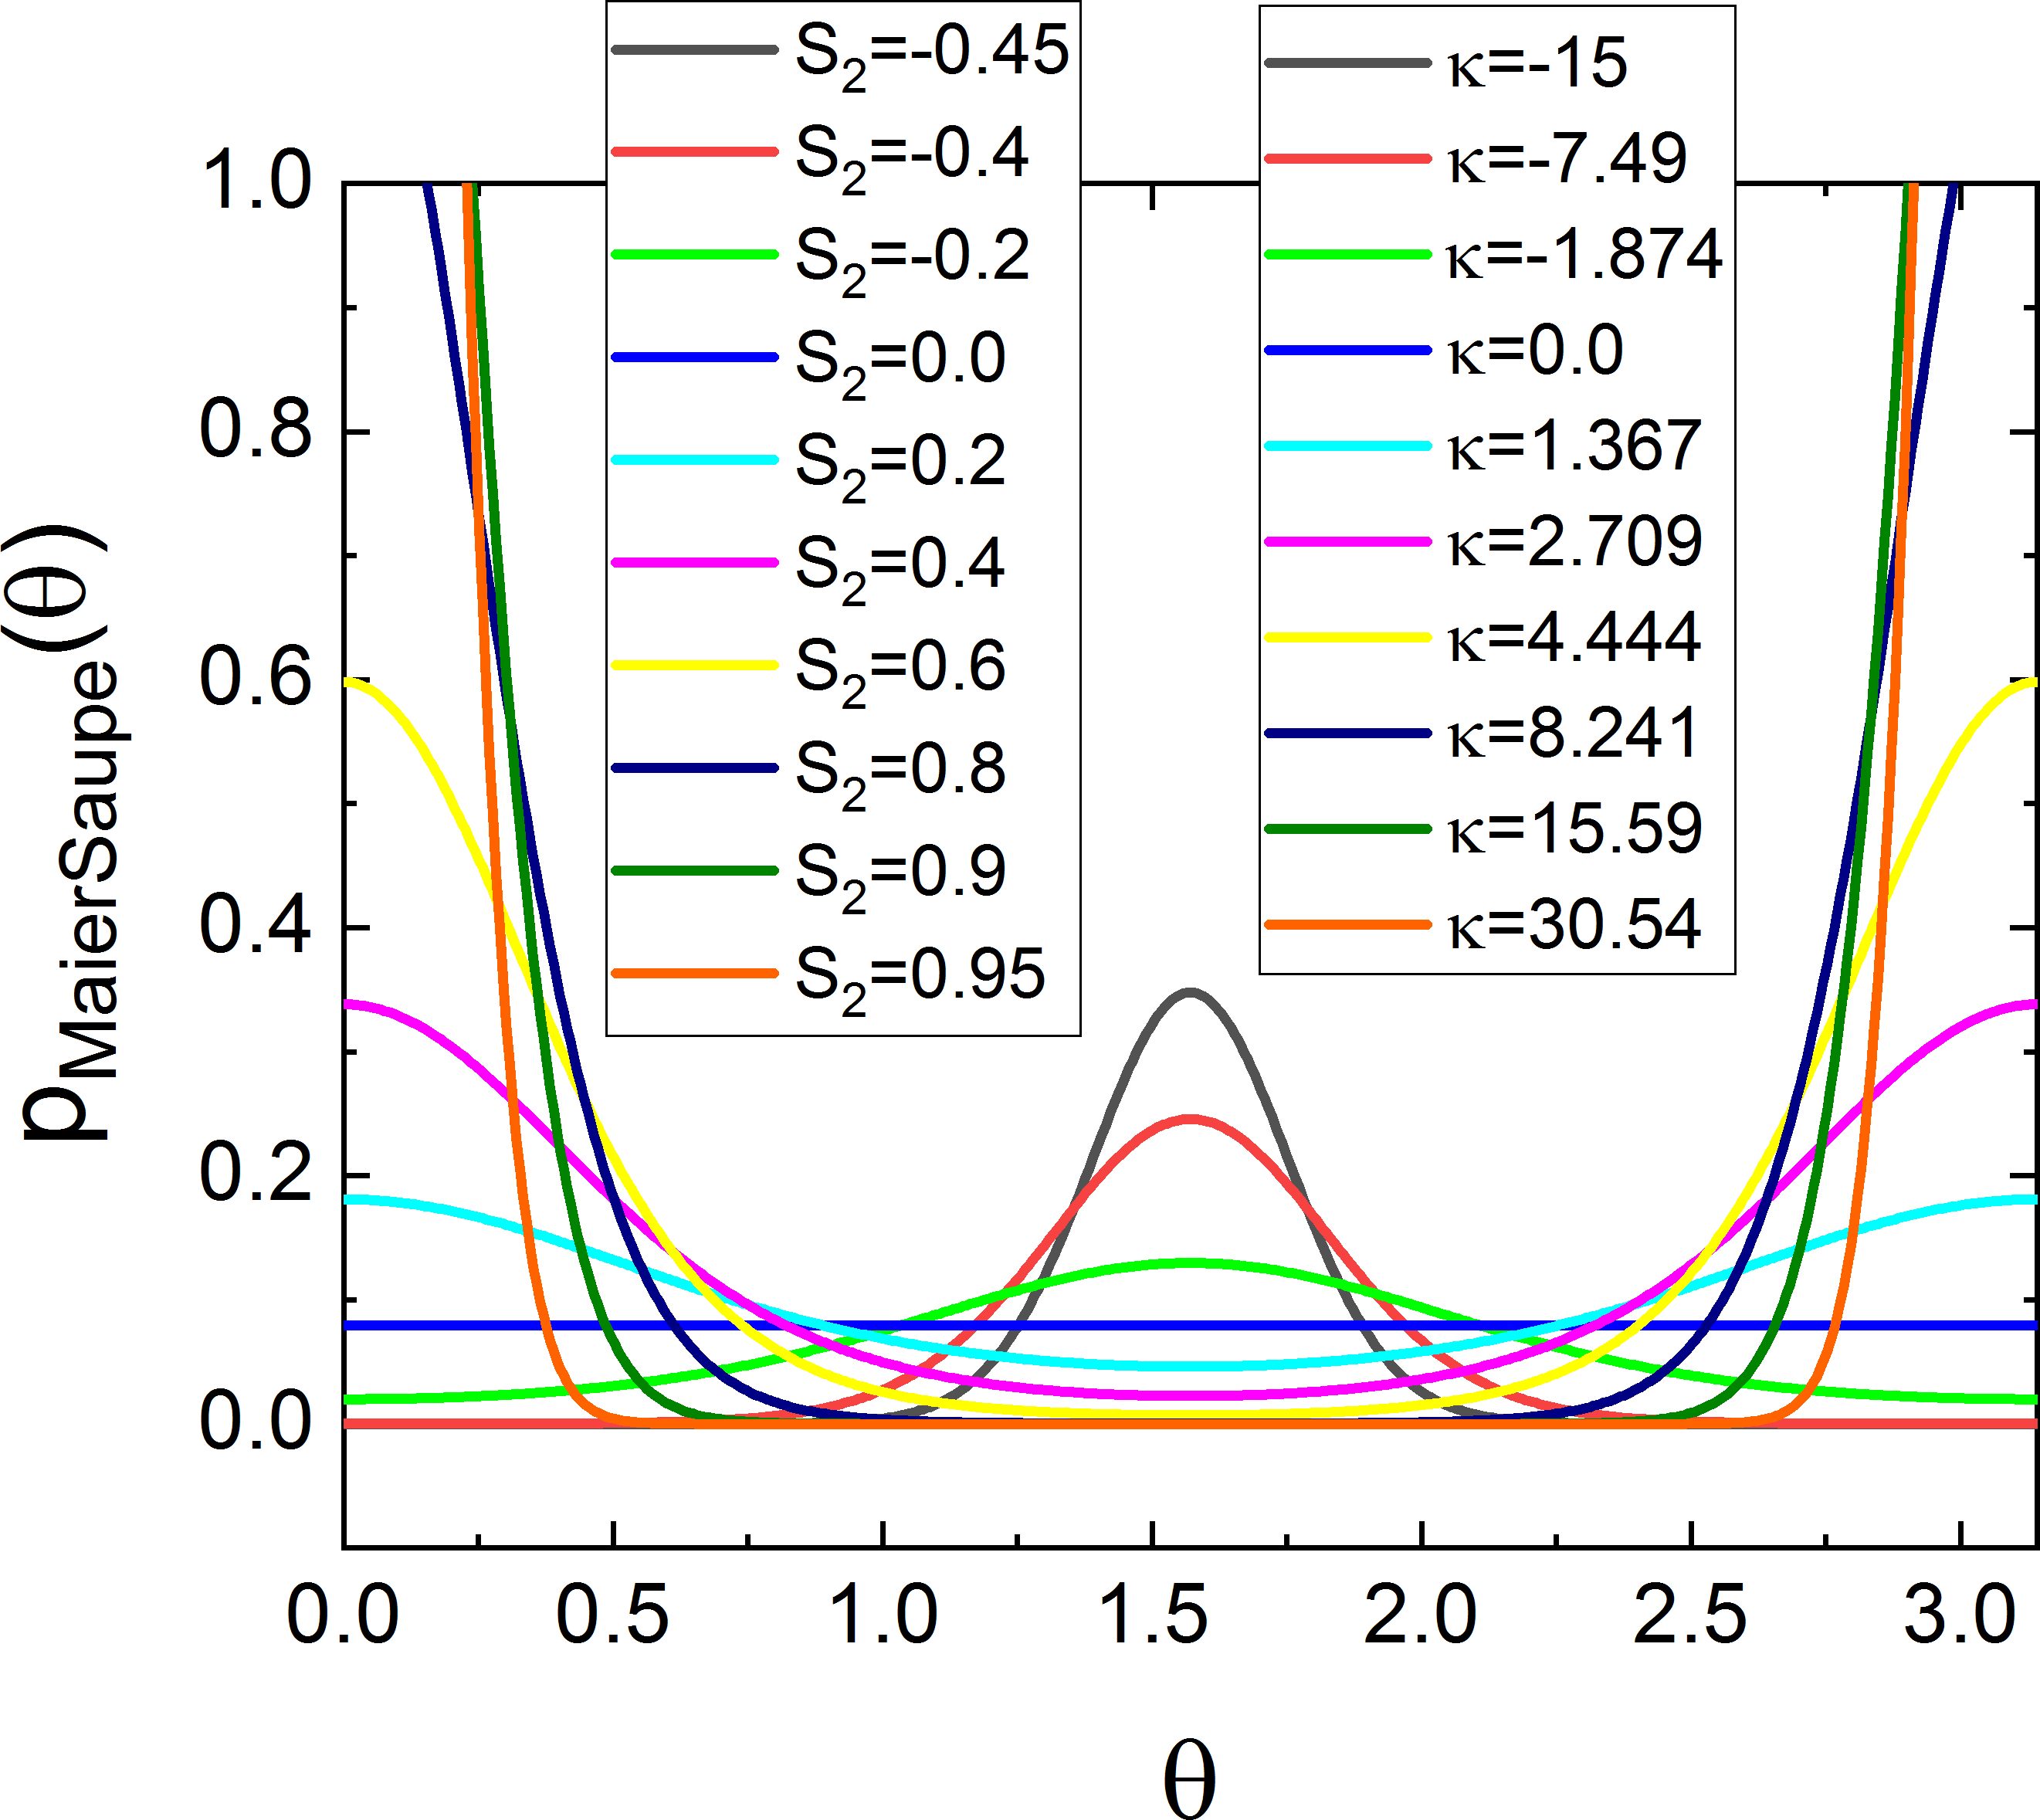
\includegraphics[width=0.75\textwidth]{../images/form_factor/cylindrical_obj/pMaierSaupeGr.png}
\caption{Maier-Saupe orientation distribution $p_\mathrm{MS}(\theta,\kappa)$ for different values of $\kappa$, resulting in an order parameter as listed in table \ref{tab:kappas}.}
\label{fig:pMaierSaupeGr}
\end{figure}

\begin{align}
p(\theta,\phi;\kappa) & = \frac{1}{c_\mathrm{MS}}\exp\left(\kappa \cos^2\theta\right)
\end{align}
with
\begin{align}
c_\mathrm{MS} &=
\begin{cases}
\displaystyle
4\pi\exp(\kappa) \frac{\mathrm{D}\left(\sqrt{\kappa}\right)}{\sqrt{\kappa}}   &\mathrm{for~} \kappa > 0 \\[5mm]
\displaystyle
2\pi \sqrt{\pi} \frac{\mathrm{erf}\left(\sqrt{\abs{\kappa}}\right)}{\sqrt{\abs{\kappa}}}  &\mathrm{for~} \kappa < 0 \\[2mm]
\displaystyle
4\pi                                                                                      &\mathrm{for~} \kappa = 0
\end{cases}
\end{align}
with $D(x)$ being Dawson's integral $D(x)=e^{-x^2}\int_0^x e^{y^2} \mathrm{d}y = \frac12\sqrt{\pi}e^{-x^2}\mathrm{erfi}(x)$

\vspace{5mm}

\uline{Input Parameters for model \texttt{Sheared Cylinders (Maier-Saupe)}:}\\
\begin{description}
\item[\texttt{R}] radius of cylinders $R$
\item[\texttt{t}] shell thickness $t$
\item[\texttt{L}] cylinder length $L$
\item[\texttt{eta\_core}] scattering length density of cylinder core $\eta_\mathrm{core}$
\item[\texttt{eta\_shell}] scattering length density of cylinder shell $\eta_\mathrm{shell}$
\item[\texttt{eta\_solv}] scattering length density of solvent $\eta_\mathrm{solv}$
\item[\texttt{psi}] direction of scattering vector on the detector $\psi$
\item[{\texttt{sigma}}] width parameter of lognormal size distribution $\sigma$
\item[{\texttt{kappa}}] orientation distribution parameter $\kappa$
\end{description}

\vspace{5mm}

\uline{Input Parameters for model \texttt{Sheared Spheroids (Maier-Saupe)}:}\\
\begin{description}
\item[\texttt{R\_equatorial}] equatorial semi-axes of spheroids $R_\mathrm{e}$
\item[\texttt{t}] shell thickness $t$
\item[\texttt{R\_polar}] polar semi-axis of spheroids $R_\mathrm{p}$
\item[\texttt{eta\_core}] scattering length density of cylinder core $\eta_\mathrm{core}$
\item[\texttt{eta\_shell}] scattering length density of cylinder shell $\eta_\mathrm{shell}$
\item[\texttt{eta\_solv}] scattering length density of solvent $\eta_\mathrm{solv}$
\item[\texttt{psi}] direction of scattering vector on the detector $\psi$
\item[{\texttt{sigma}}] width parameter of lognormal size distribution $\sigma$
\item[{\texttt{kappa}}] orientation distribution parameter $\kappa$
\end{description}

\vspace{5mm}

\uline{Note:}
\begin{itemize}
\item The size distribution is taken simultaneously over all parameters $R$, $t$, $L$, and $R_\mathrm{e}$, $t$, $R_\mathrm{p}$ respectively, so that their aspect ratios always stay constant.
\end{itemize}
%%%%%%%%%%%%%%%%%%%%%%%%%%%%%%%%%%%%%%%%%%%%%%%%%%%%%%%%%%%%%%%%%%%%%%%%%%%%%%%%%%

\newpage
\subsubsection{Onsager orientation distribution} ~\\

\begin{figure}[htb]
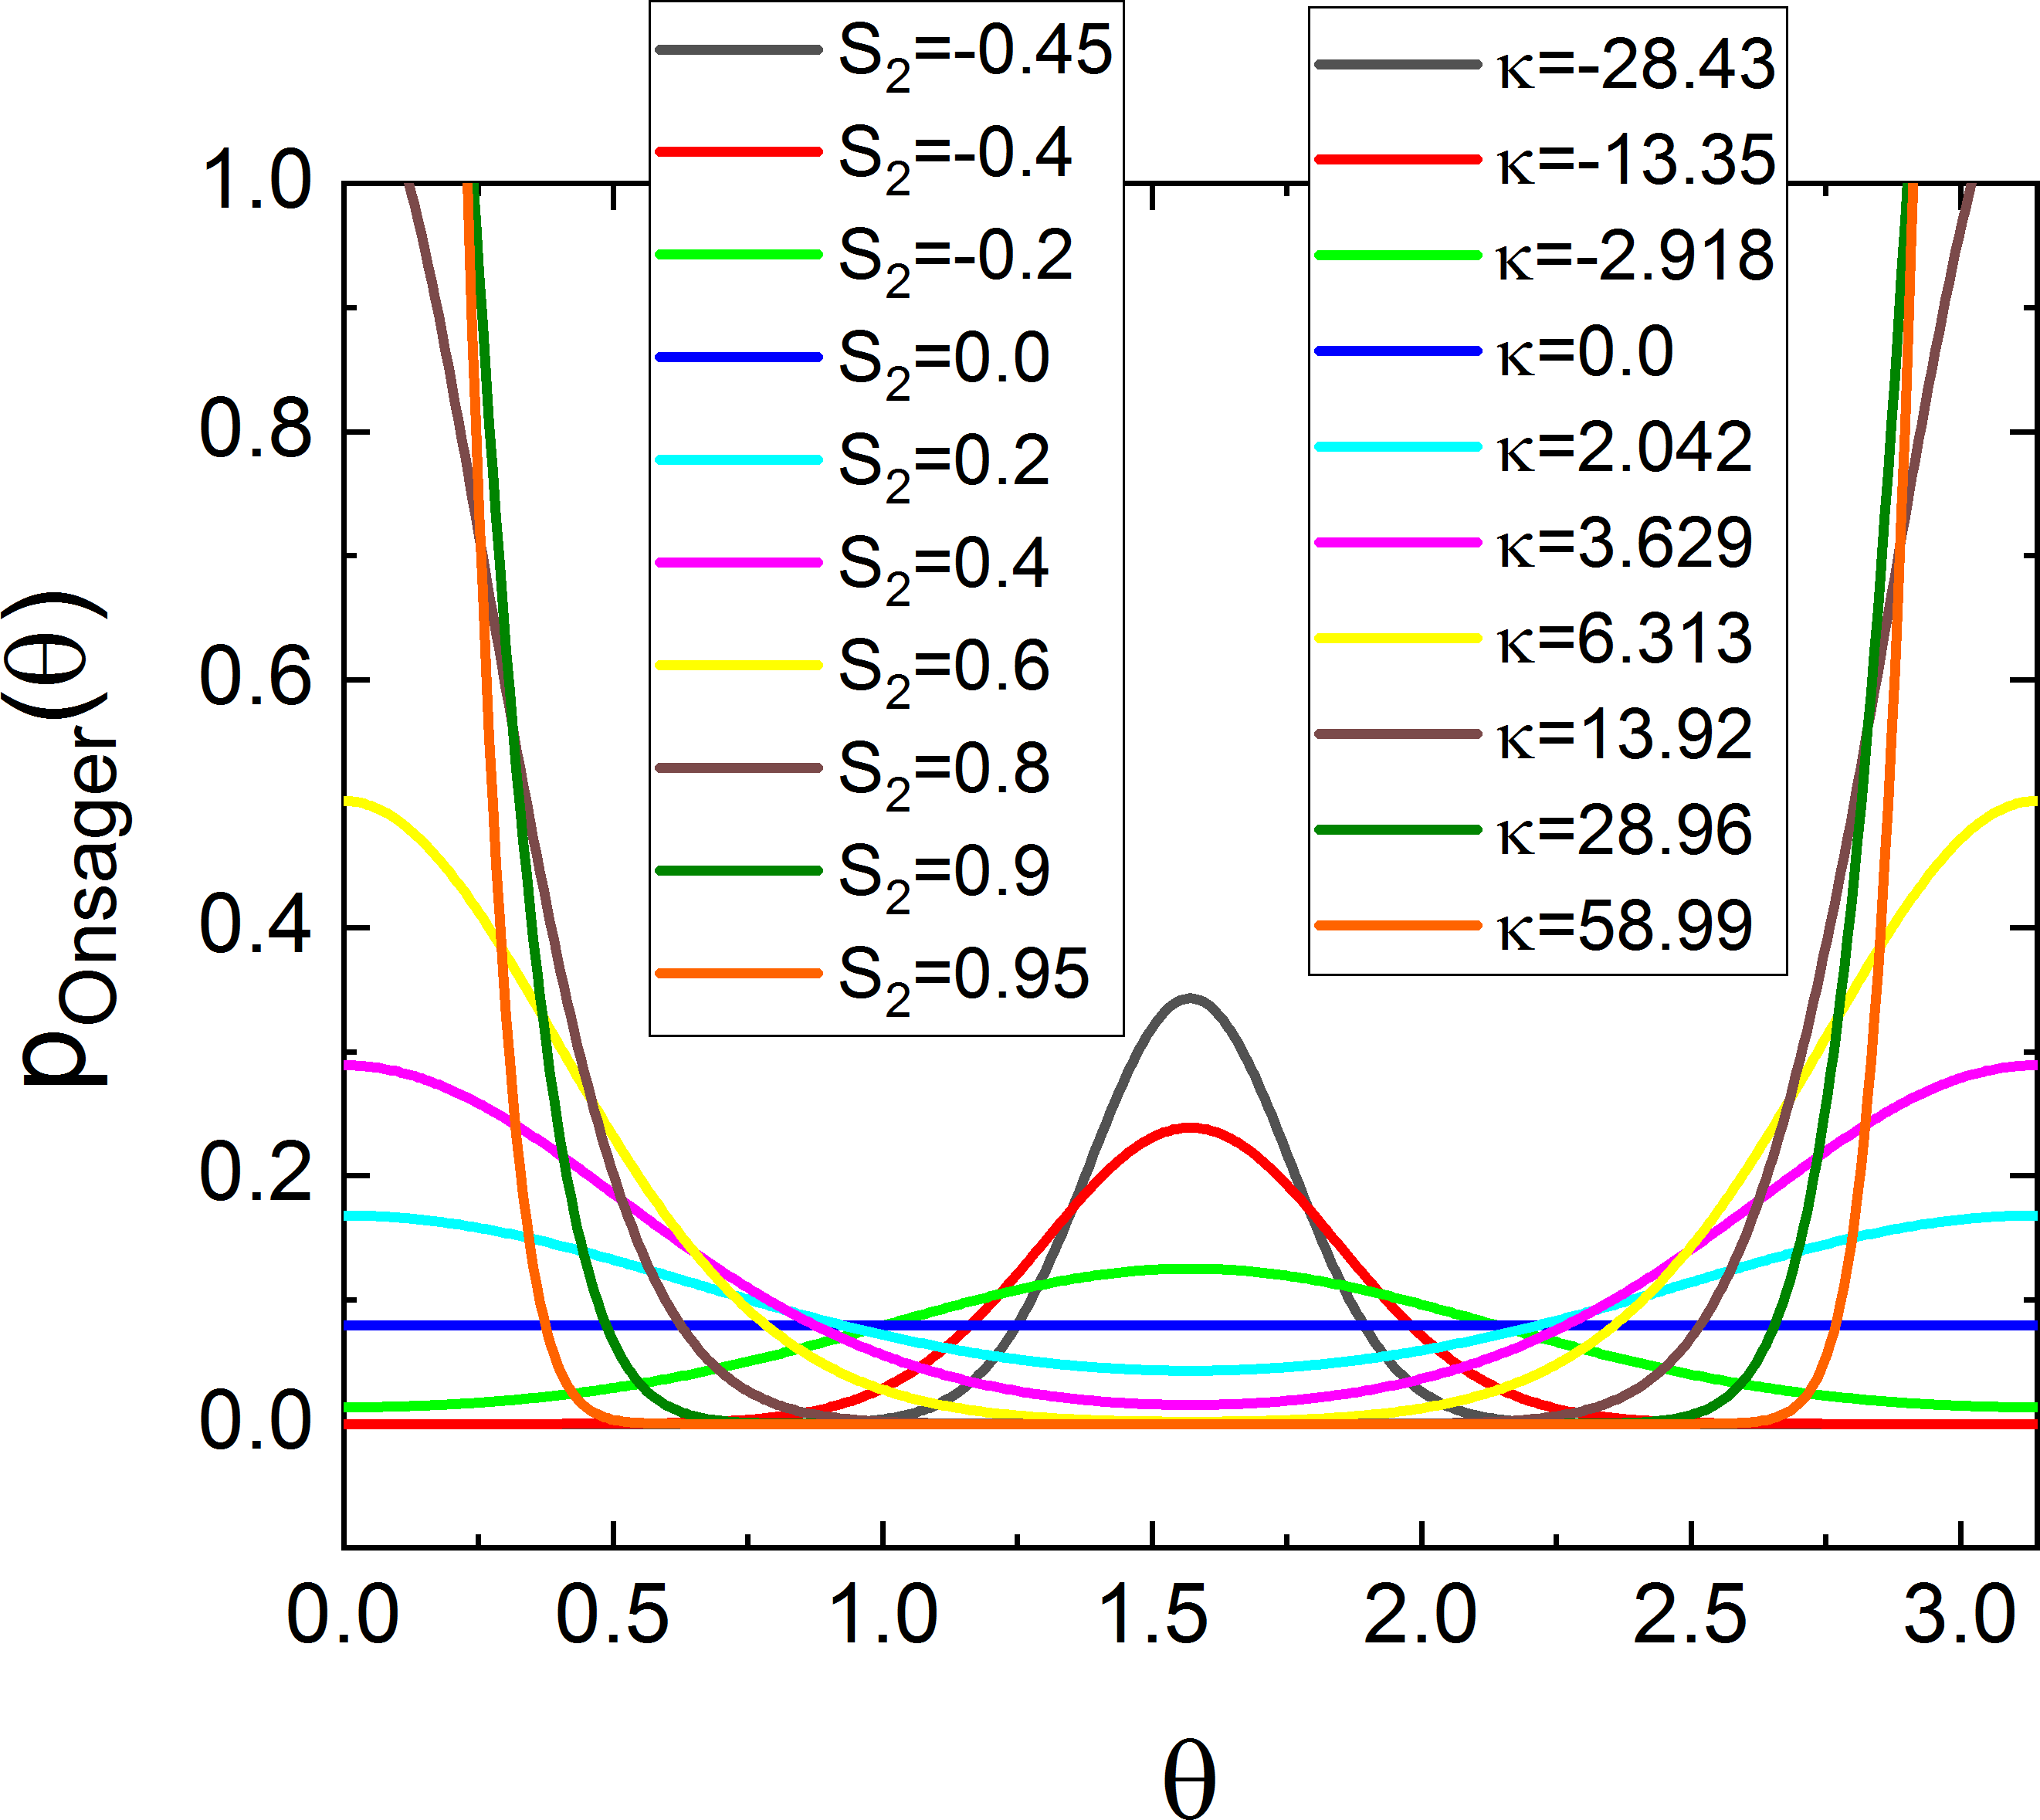
\includegraphics[width=0.75\textwidth]{../images/form_factor/cylindrical_obj/pOnsagerGr.png}
\caption{Onsager orientation distribution $p_\mathrm{O}(\theta,\kappa)$ for different values of $\kappa$, resulting in an order parameter as listed in table \ref{tab:kappas}.}
\label{fig:pOnsagerGr}
\end{figure}

\begin{align}
p_\mathrm{O}(\theta,\phi;\kappa) & =
\begin{cases} \displaystyle
\frac{\kappa \cosh\left(\kappa \cos(\theta)\right)}{4\pi \sinh(\kappa)}      &\mathrm{for~} \kappa \geq 0 \\[5mm]
 \displaystyle
\frac{\cosh\left(\abs{\kappa} \sin(\theta)\right)}{2\pi^2 L_1(\abs{\kappa})}  &\mathrm{for~} \kappa < 0
\end{cases}
\end{align}
where $L_\nu(x)$ is the modified Struve function.

\vspace{5mm}

\uline{Input Parameters for model \texttt{Sheared Cylinders (Onsager)}:}\\
\begin{description}
\item[\texttt{R}] radius of cylinders $R$
\item[\texttt{t}] shell thickness $t$
\item[\texttt{L}] cylinder length $L$
\item[\texttt{eta\_core}] scattering length density of cylinder core $\eta_\mathrm{core}$
\item[\texttt{eta\_shell}] scattering length density of cylinder shell $\eta_\mathrm{shell}$
\item[\texttt{eta\_solv}] scattering length density of solvent $\eta_\mathrm{solv}$
\item[\texttt{psi}] direction of scattering vector on the detector $\psi$
\item[{\texttt{sigma}}] width parameter of lognormal size distribution $\sigma$
\item[{\texttt{kappa}}] orientation distribution parameter $\kappa$
\end{description}

\vspace{5mm}

\uline{Input Parameters for model \texttt{Sheared Spheroids (Onsager}:}\\
\begin{description}
\item[\texttt{R\_equatorial}] equatorial semi-axes of spheroids $R_\mathrm{e}$
\item[\texttt{t}] shell thickness $t$
\item[\texttt{R\_polar}] polar semi-axis of spheroids $R_\mathrm{p}$
\item[\texttt{eta\_core}] scattering length density of cylinder core $\eta_\mathrm{core}$
\item[\texttt{eta\_shell}] scattering length density of cylinder shell $\eta_\mathrm{shell}$
\item[\texttt{eta\_solv}] scattering length density of solvent $\eta_\mathrm{solv}$
\item[\texttt{psi}] direction of scattering vector on the detector $\psi$
\item[{\texttt{sigma}}] width parameter of lognormal size distribution $\sigma$
\item[{\texttt{kappa}}] orientation distribution parameter $\kappa$
\end{description}

\vspace{5mm}

\uline{Note:}
\begin{itemize}
\item The size distribution is taken simultaneously over all parameters $R$, $t$, $L$, and $R_\mathrm{e}$, $t$, $R_\mathrm{p}$ respectively, so that their aspect ratios always stay constant.
\end{itemize}
%%%%%%%%%%%%%%%%%%%%%%%%%%%%%%%%%%%%%%%%%%%%%%%%%%%%%%%%%%%%%%%%%%%%%%%%%%%%%%%%%%

\newpage
\subsubsection{Boltzmann orientation distribution} ~\\

\begin{figure}[htb]
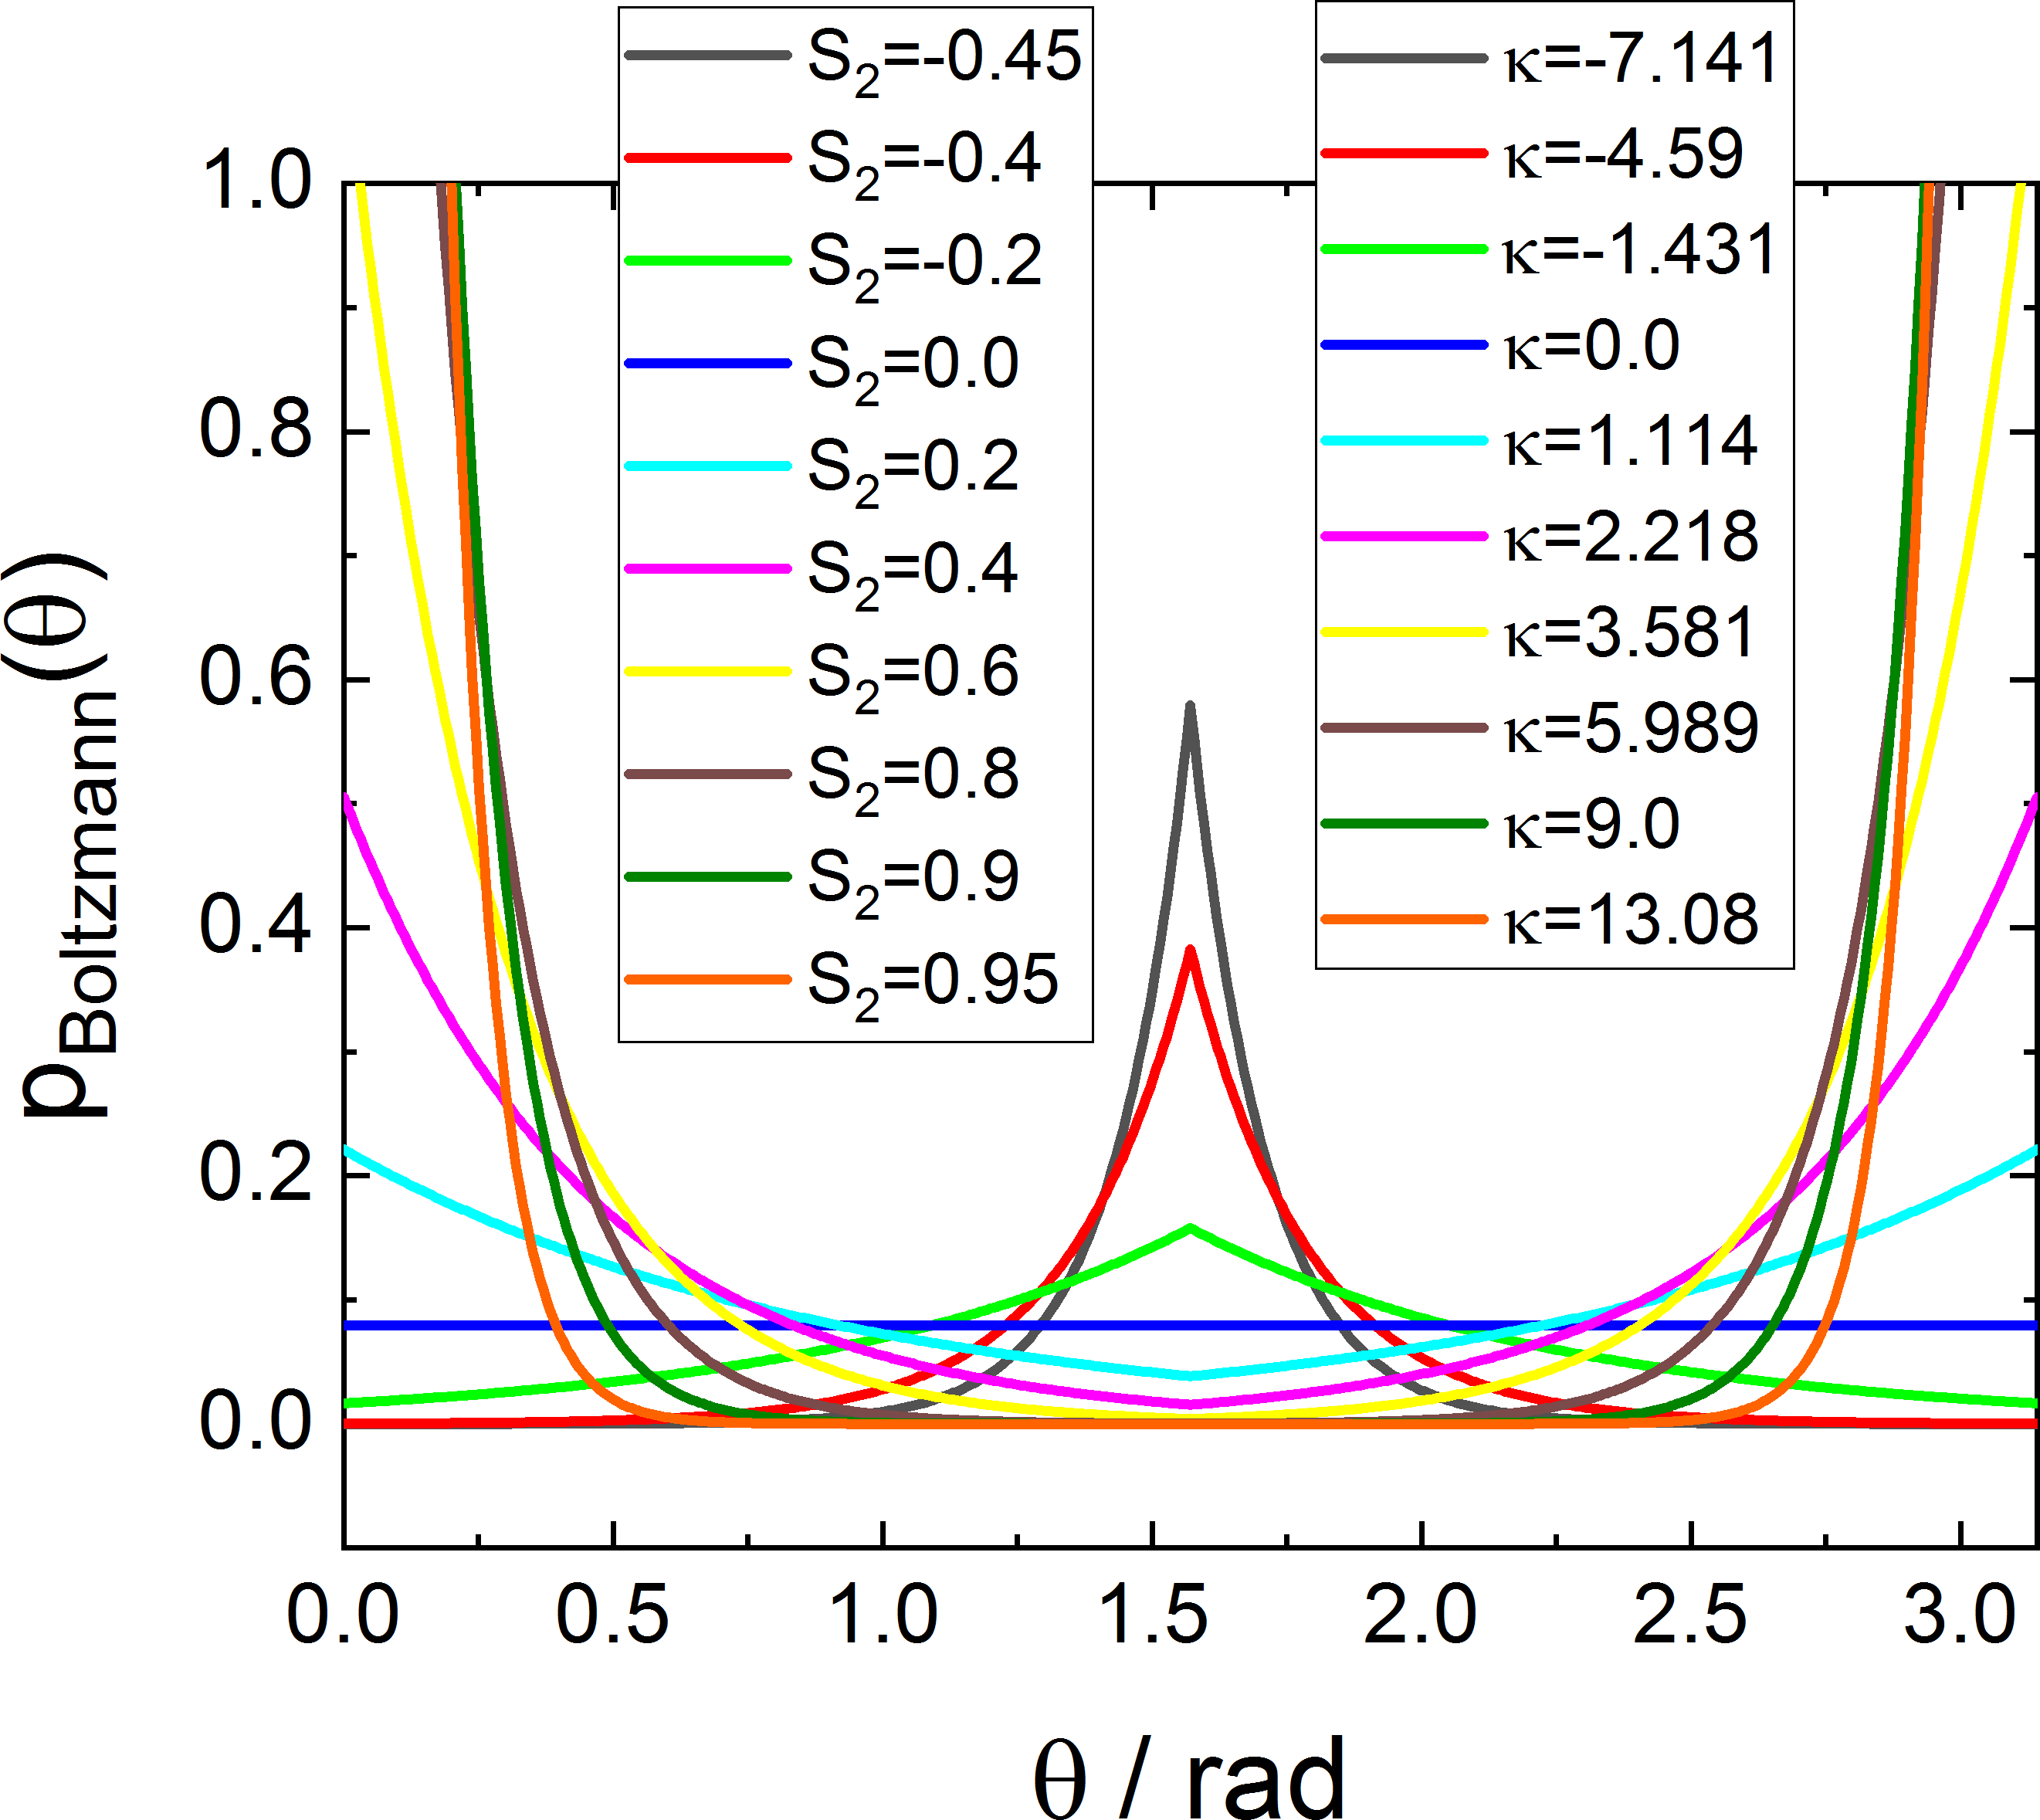
\includegraphics[width=0.75\textwidth]{../images/form_factor/cylindrical_obj/pBoltzmannGr.png}
\caption{Boltzmann orientation distribution $p_\mathrm{B}(\theta,\kappa)$ for different values of $\kappa$, resulting in an order parameter as listed in table \ref{tab:kappas}.}
\label{fig:pBoltzmannGr}
\end{figure}

\begin{align}
p_\mathrm{B}(\theta,\phi;\kappa) & =
\begin{cases}
\displaystyle
\frac{1}{2\pi c_\mathrm{B}}\exp\left(-\theta\kappa\right) & \mathrm{for~}  \theta \leq \frac{\pi}{2}\\[5mm]
\displaystyle
\frac{1}{2\pi c_\mathrm{B}}\exp\left(-(\pi-\theta)\kappa\right) & \mathrm{for~}  \theta > \frac{\pi}{2}
\end{cases}
\end{align}
with
\begin{align}
c_\mathrm{B} &= \frac{2\left(1-\kappa \exp\left(-\frac{\pi}{2}\kappa\right)\right)}{\kappa^2+1}
\end{align}

\vspace{5mm}

\uline{Input Parameters for model \texttt{Sheared Cylinders (Boltzmann)}:}\\
\begin{description}
\item[\texttt{R}] radius of cylinders $R$
\item[\texttt{t}] shell thickness $t$
\item[\texttt{L}] cylinder length $L$
\item[\texttt{eta\_core}] scattering length density of cylinder core $\eta_\mathrm{core}$
\item[\texttt{eta\_shell}] scattering length density of cylinder shell $\eta_\mathrm{shell}$
\item[\texttt{eta\_solv}] scattering length density of solvent $\eta_\mathrm{solv}$
\item[\texttt{psi}] direction of scattering vector on the detector $\psi$
\item[{\texttt{sigma}}] width parameter of lognormal size distribution $\sigma$
\item[{\texttt{kappa}}] orientation distribution parameter $\kappa$
\end{description}

\vspace{5mm}

\uline{Input Parameters for model \texttt{Sheared Spheroids (Boltzmann)}:}\\
\begin{description}
\item[\texttt{R\_equatorial}] equatorial semi-axes of spheroids $R_\mathrm{e}$
\item[\texttt{t}] shell thickness $t$
\item[\texttt{R\_polar}] polar semi-axis of spheroids $R_\mathrm{p}$
\item[\texttt{eta\_core}] scattering length density of cylinder core $\eta_\mathrm{core}$
\item[\texttt{eta\_shell}] scattering length density of cylinder shell $\eta_\mathrm{shell}$
\item[\texttt{eta\_solv}] scattering length density of solvent $\eta_\mathrm{solv}$
\item[\texttt{psi}] direction of scattering vector on the detector $\psi$
\item[{\texttt{sigma}}] width parameter of lognormal size distribution $\sigma$
\item[{\texttt{kappa}}] orientation distribution parameter $\kappa$
\end{description}

\vspace{5mm}

\uline{Note:}
\begin{itemize}
\item The size distribution is taken simultaneously over all parameters $R$, $t$, $L$, and $R_\mathrm{e}$, $t$, $R_\mathrm{p}$ respectively, so that their aspect ratios always stay constant.
\end{itemize}
%%%%%%%%%%%%%%%%%%%%%%%%%%%%%%%%%%%%%%%%%%%%%%%%%%%%%%%%%%%%%%%%%%%%%%%%%%%%%%%%%%

\newpage
\subsubsection{Gaussian orientation distribution}
\label{sect:ShearedCylinderGaussian}
~\\

\begin{figure}[htb]
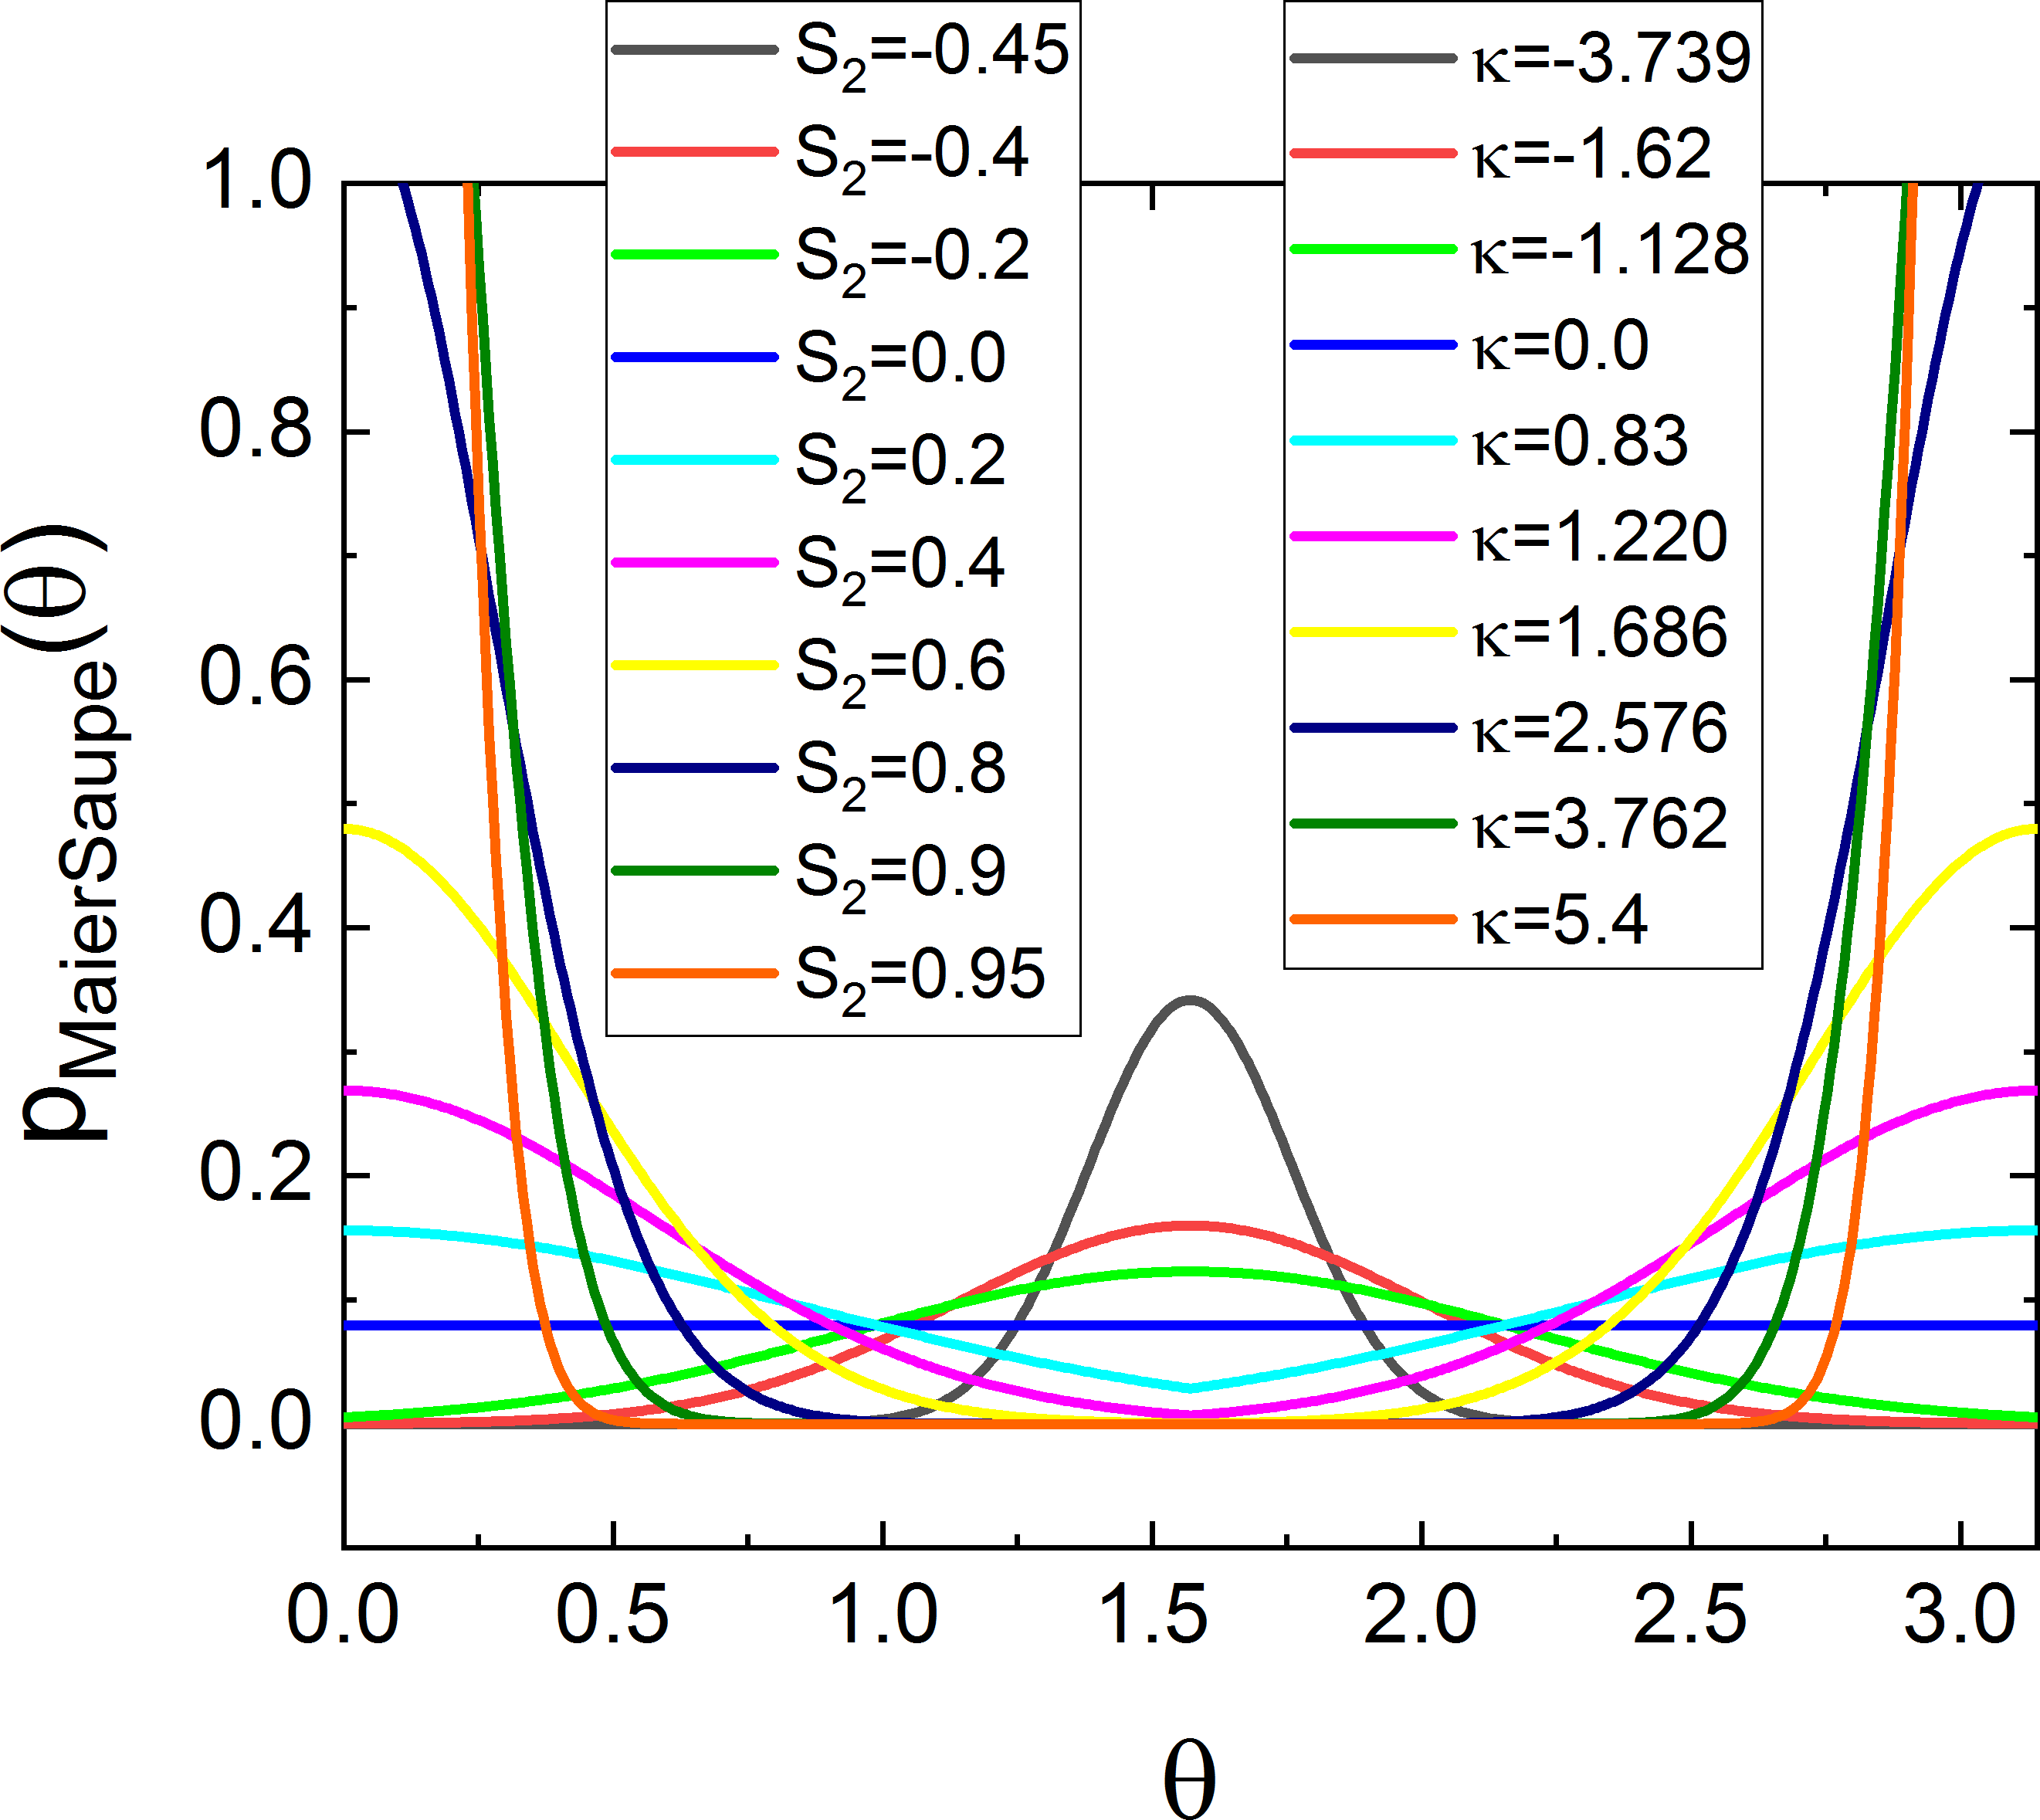
\includegraphics[width=0.75\textwidth]{../images/form_factor/cylindrical_obj/pGaussGr.png}
\caption{Gaussian orientation distribution $p_\mathrm{G}(\theta,\kappa)$ for different values of $\kappa$, resulting in an order parameter as listed in table \ref{tab:kappas}.}
\label{fig:pGaussGr}
\end{figure}

\begin{align}
p_\mathrm{G}(\theta,\phi;\kappa) & =
\begin{cases}
\displaystyle
\frac{1}{2\pi c_\mathrm{G}}\exp\left(-\theta^2\kappa^2\right) & \mathrm{for~} \kappa \geq 0 \mathrm{~and~} \theta \leq \frac{\pi}{2}\\[5mm]
\displaystyle
\frac{1}{2\pi c_\mathrm{G}}\exp\left(-\left(\pi-\theta\right)^2\kappa^2\right) & \mathrm{for~} \kappa \geq 0 \mathrm{~and~} \theta > \frac{\pi}{2}\\[5mm]
\displaystyle
\frac{1}{2\pi c_\mathrm{G}}\exp\left(-\left(\frac{\pi}{2}-\theta\right)^2\abs{\kappa}^2\right) & \mathrm{for~} \kappa < 0
\end{cases}
\end{align}
with
\begin{align}
c_\mathrm{G} & =
\begin{cases}\displaystyle
\frac{D\left(\kappa/2\right)}{\kappa}
           +\frac{\sqrt{\pi}}{2\kappa} e^{-\frac{1}{4\kappa^2}} \Re\left(\mathrm{cerfi}\left(-\frac{1}{2\kappa}+\imath\frac{\pi}{2}\kappa\right) \right)& \mathrm{for~} \kappa \geq 0 \\[5mm]
\displaystyle
\frac{\sqrt{\pi}}{\abs{\kappa}} e^{-\frac{1}{4\kappa^2}} \Im\left(\mathrm{cerfi}\left(-\frac{1}{2\abs{\kappa}}+\imath\frac{\pi}{2}\abs{\kappa}\right) \right) & \mathrm{for~} \kappa < 0
\end{cases}
\end{align}

\vspace{5mm}

\uline{Input Parameters for model \texttt{Sheared Cylinders (Gauss)}:}\\
\begin{description}
\item[\texttt{R}] radius of cylinders $R$
\item[\texttt{t}] shell thickness $t$
\item[\texttt{L}] cylinder length $L$
\item[\texttt{eta\_core}] scattering length density of cylinder core $\eta_\mathrm{core}$
\item[\texttt{eta\_shell}] scattering length density of cylinder shell $\eta_\mathrm{shell}$
\item[\texttt{eta\_solv}] scattering length density of solvent $\eta_\mathrm{solv}$
\item[\texttt{psi}] direction of scattering vector on the detector $\psi$
\item[{\texttt{sigma}}] width parameter of lognormal size distribution $\sigma$
\item[{\texttt{kappa}}] orientation distribution parameter $\kappa$
\end{description}

\vspace{5mm}

\uline{Input Parameters for model \texttt{Sheared Spheroids (Gauss)}:}\\
\begin{description}
\item[\texttt{R\_equatorial}] equatorial semi-axes of spheroids $R_\mathrm{e}$
\item[\texttt{t}] shell thickness $t$
\item[\texttt{R\_polar}] polar semi-axis of spheroids $R_\mathrm{p}$
\item[\texttt{eta\_core}] scattering length density of cylinder core $\eta_\mathrm{core}$
\item[\texttt{eta\_shell}] scattering length density of cylinder shell $\eta_\mathrm{shell}$
\item[\texttt{eta\_solv}] scattering length density of solvent $\eta_\mathrm{solv}$
\item[\texttt{psi}] direction of scattering vector on the detector $\psi$
\item[{\texttt{sigma}}] width parameter of lognormal size distribution $\sigma$
\item[{\texttt{kappa}}] orientation distribution parameter $\kappa$
\end{description}

\vspace{5mm}

\uline{Note:}
\begin{itemize}
\item The size distribution is taken simultaneously over all parameters $R$, $t$, $L$, and $R_\mathrm{e}$, $t$, $R_\mathrm{p}$ respectively, so that their aspect ratios always stay constant.
\end{itemize}

%%%%%%%%%%%%%%%%%%%%%%%%%%%%%%%%%%%%%%%%%%%%%%%%%%%%%%%%%%%%%%%%%%%%%%%%%%%%%%%%%%

\newpage
\subsubsection{Boxed orientation distribution (HeavisidePi)} ~\\

\begin{figure}[htb]
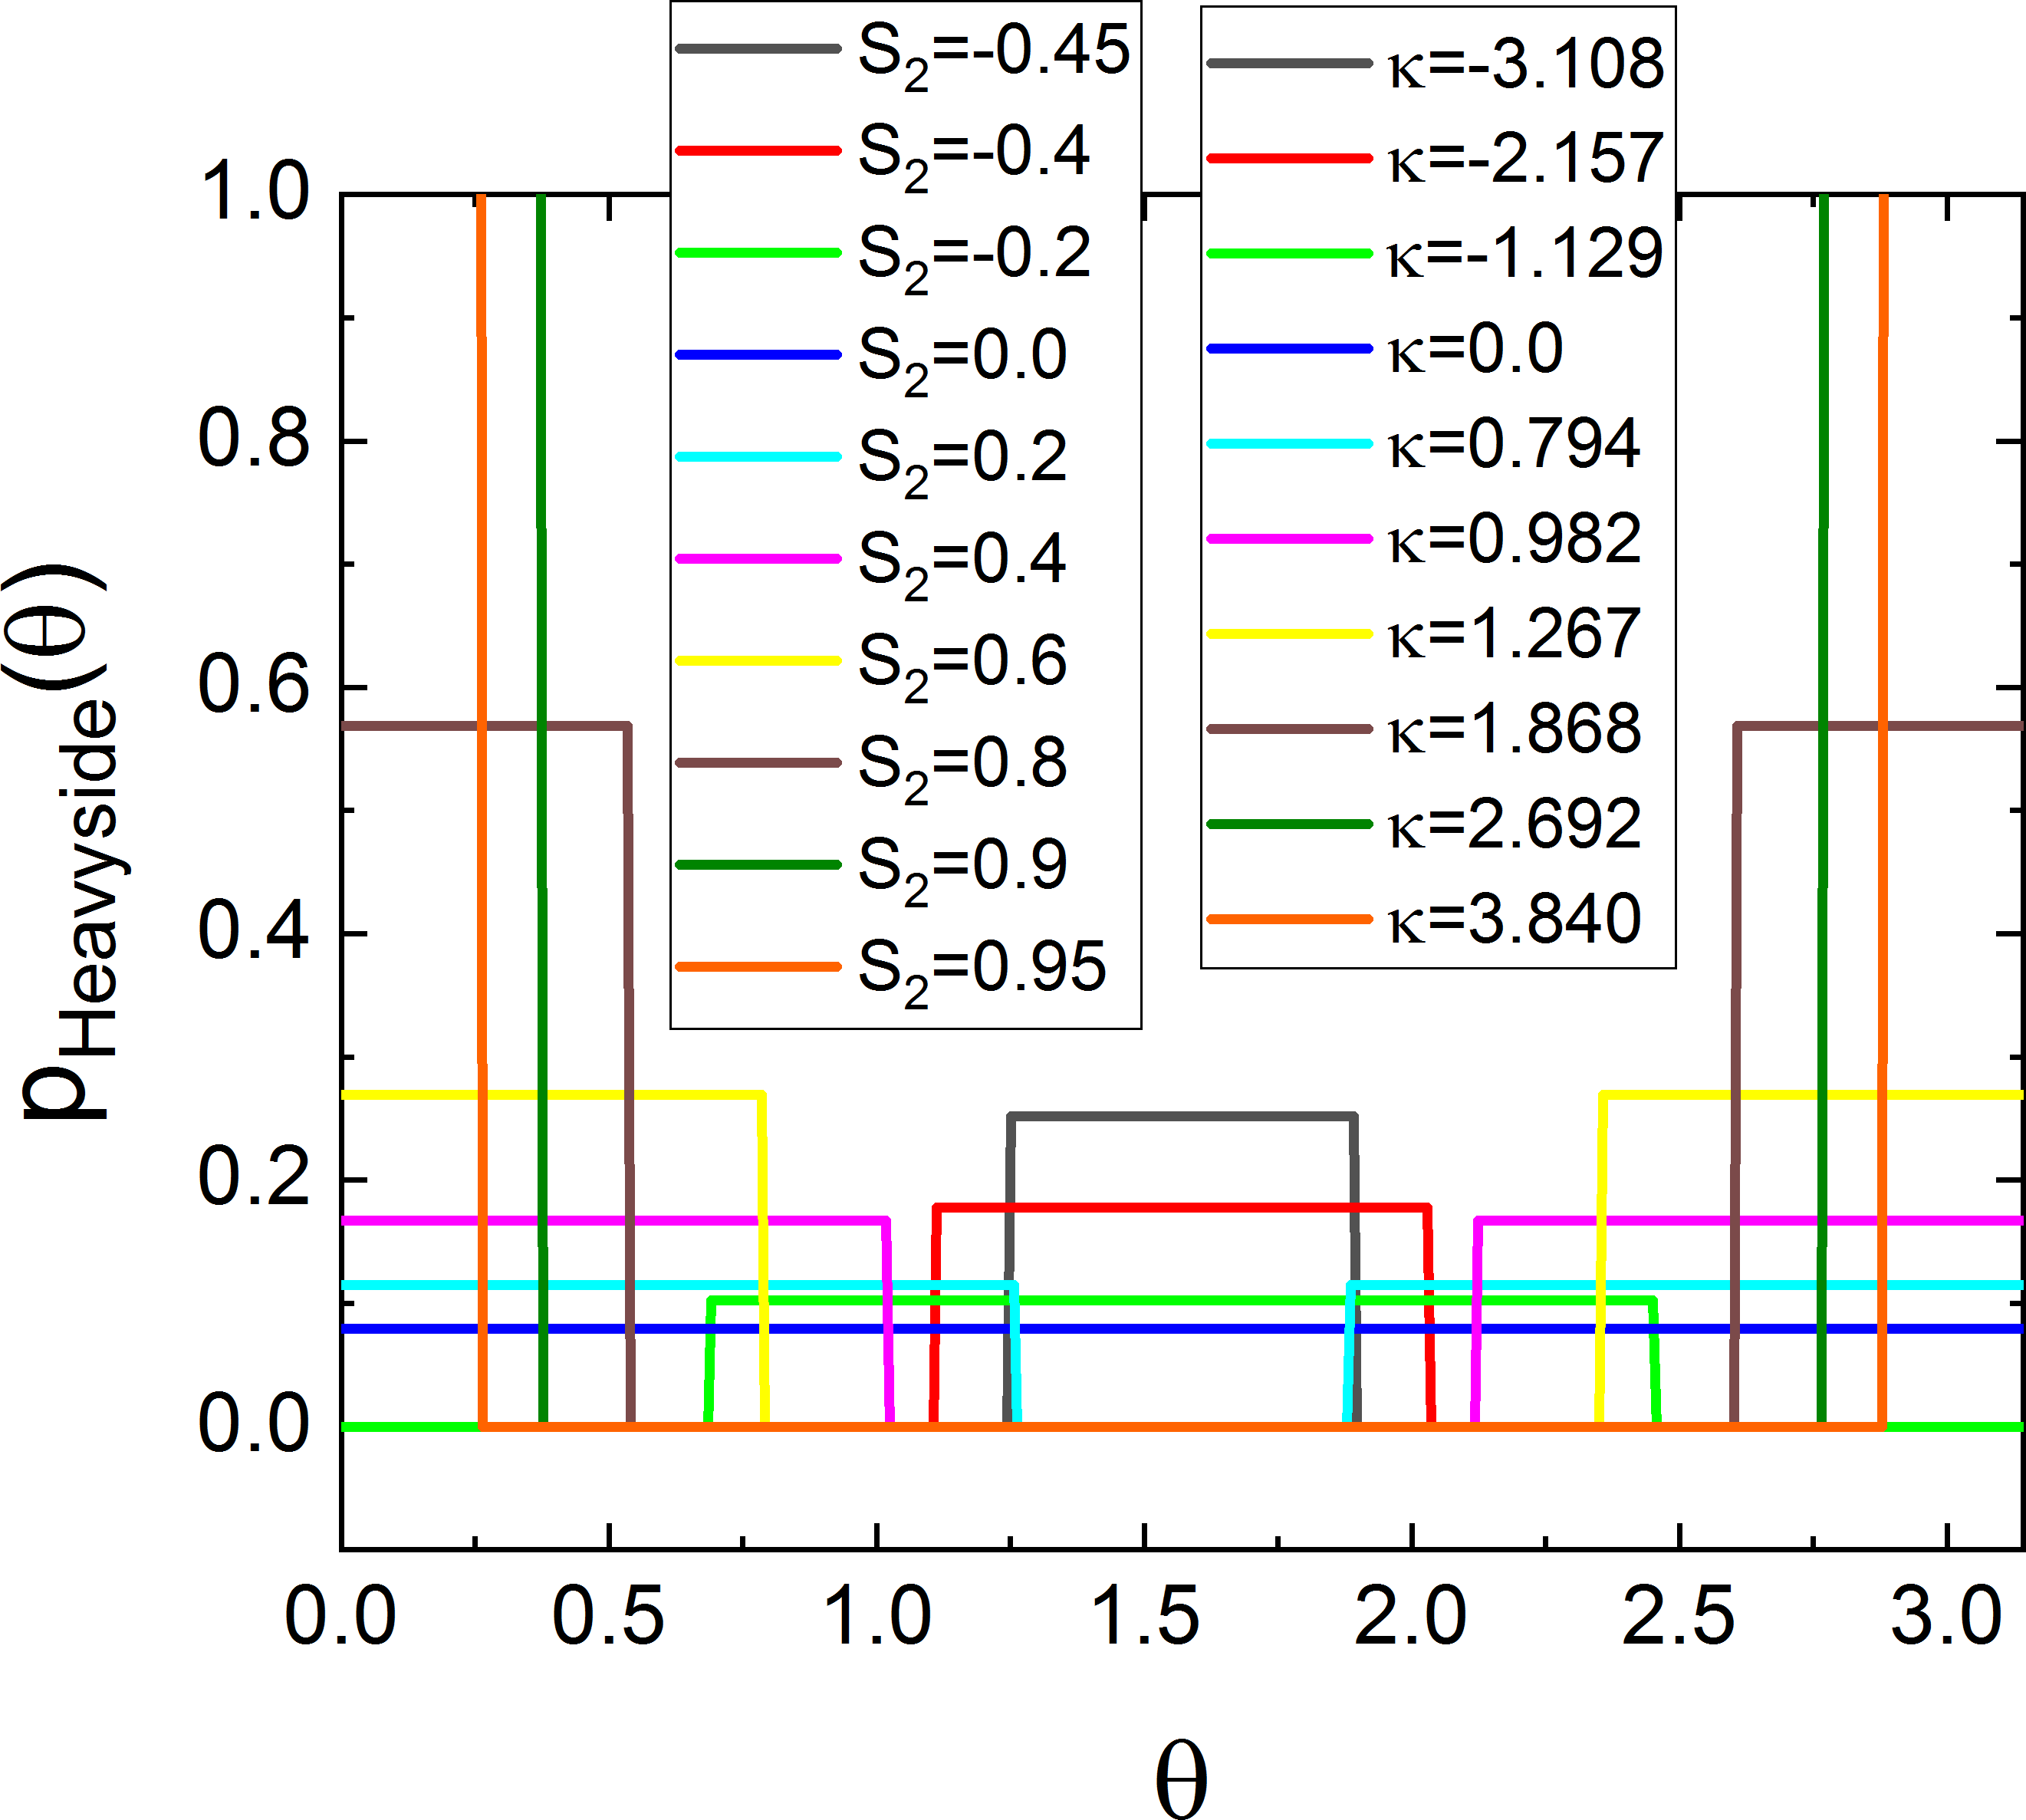
\includegraphics[width=0.75\textwidth]{../images/form_factor/cylindrical_obj/pHeavisideGr.png}
\caption{Heaviside orientation distribution $p_\mathrm{HS}(\theta,\kappa)$ for different values of $\kappa$, resulting in an order parameter as listed in table \ref{tab:kappas}.}
\label{fig:pHeavisideGr}
\end{figure}


\begin{align}
p(\theta,\phi;\kappa) & =
\begin{cases}
\displaystyle
\frac{1}{4\pi\left(1-\cos\left(1/\kappa\right)\right)}\left(\Pi\left(\frac{x\kappa}{2}\right) + \Pi\left(\frac{(x-\pi)\kappa}{2}\right)\right)
 & \mathrm{for~} \kappa >  \frac{2}{\pi}
 \\[5mm]
\displaystyle
 \frac{1}{4\pi} & \mathrm{for~}  \abs{\kappa} \leq \frac{2}{\pi}
 \\[5mm]
\displaystyle
 \frac{1}{4\pi\sin\left(\frac{1}{\abs{\kappa}}\right)} \Pi\left(\frac{\left(x-\frac{\pi}{2}\right)\abs{\kappa}}{2}\right) & \mathrm{for~}  \kappa<-\frac{2}{\pi}
\end{cases}
\end{align}
with the rectangle function $\Pi(x)$
\begin{align}
\Pi(x) &=
\begin{cases}
\displaystyle
0 & \mathrm{for~} \abs{x} > \frac12
 \\[5mm]
\displaystyle
\frac12 & \mathrm{for~}  \abs{x} = \frac12
 \\[5mm]
\displaystyle
 1 & \mathrm{for~}  \abs{x} < \frac12
\end{cases}
\end{align}

\vspace{5mm}

\uline{Input Parameters for model \texttt{Sheared Cylinders (Heaviside)}:}\\
\begin{description}
\item[\texttt{R}] radius of cylinders $R$
\item[\texttt{t}] shell thickness $t$
\item[\texttt{L}] cylinder length $L$
\item[\texttt{eta\_core}] scattering length density of cylinder core $\eta_\mathrm{core}$
\item[\texttt{eta\_shell}] scattering length density of cylinder shell $\eta_\mathrm{shell}$
\item[\texttt{eta\_solv}] scattering length density of solvent $\eta_\mathrm{solv}$
\item[\texttt{psi}] direction of scattering vector on the detector $\psi$
\item[{\texttt{sigma}}] width parameter of lognormal size distribution $\sigma$
\item[{\texttt{kappa}}] orientation distribution parameter $\kappa$
\end{description}

\vspace{5mm}

\uline{Input Parameters for model \texttt{Sheared Spheroids (Heaviside)}:}\\
\begin{description}
\item[\texttt{R\_equatorial}] equatorial semi-axes of spheroids $R_\mathrm{e}$
\item[\texttt{t}] shell thickness $t$
\item[\texttt{R\_polar}] polar semi-axis of spheroids $R_\mathrm{p}$
\item[\texttt{eta\_core}] scattering length density of cylinder core $\eta_\mathrm{core}$
\item[\texttt{eta\_shell}] scattering length density of cylinder shell $\eta_\mathrm{shell}$
\item[\texttt{eta\_solv}] scattering length density of solvent $\eta_\mathrm{solv}$
\item[\texttt{psi}] direction of scattering vector on the detector $\psi$
\item[{\texttt{sigma}}] width parameter of lognormal size distribution $\sigma$
\item[{\texttt{kappa}}] orientation distribution parameter $\kappa$
\end{description}

\vspace{5mm}

\uline{Note:}
\begin{itemize}
\item The size distribution is taken simultaneously over all parameters $R$, $t$, $L$, and $R_\mathrm{e}$, $t$, $R_\mathrm{p}$ respectively, so that their aspect ratios always stay constant.
\item For $\abs{\kappa}<\frac{2}{\pi}$ the partial derivative $\delta /\delta\kappa$ of the model function is zero which will cause an error message in the minimization routine. This means the fitting procedure will not work in this domain of values.
\end{itemize}
